\documentclass[a4paper,10pt,oneside,fleqn]{jsbook}
%
\usepackage{amsmath,amssymb,bm}
\usepackage{bm}
\usepackage{graphicx}
\usepackage{ascmac}
\usepackage{makeidx}
\usepackage{txfonts}
\usepackage{indentfirst}
\usepackage{indent}
\usepackage{booktabs}
\usepackage{comment}
\usepackage{cite}
\usepackage{subfigure}
\usepackage{float}
\usepackage{alltt}
\usepackage{eclbkbox,fancybox}
%
\newcounter{program}
%\bkcounttrue
\newenvironment{program}%
{\vspace{0.5\baselineskip}\VerbatimEnvironment%
%\begin{breakbox}\setlength{\baselineskip}{0pt}\begin{Verbatim}}%
\begin{breakbox}\setlength{\baselineskip}{.25\normalbaselineskip}\begin{Verbatim}}%
{\end{Verbatim}\end{breakbox}\vspace{0.8\baselineskip}}

\makeindex
%
\newcommand{\diff}{\mathrm{d}}  %微分記号
\newcommand{\divergence}{\mathrm{div}\,}  %ダイバージェンス
\newcommand{\grad}{\mathrm{grad}\,}  %グラディエント
\newcommand{\rot}{\mathrm{rot}\,}  %ローテーション
%
\setlength{\textwidth}{\fullwidth}
\setlength{\textheight}{44\baselineskip}
\addtolength{\textheight}{\topskip}
\setlength{\voffset}{-0.6in}
\setlength{\mathindent}{1.5cm} %数式のインデント設定
\setcounter{secnumdepth}{2} %subsectionまで番号付け
\setcounter{tocdepth}{4} %目次の深さ設定
\renewcommand\citemid{; } %citeのオプション

%subfigure
\renewcommand{\subfigtopskip}{5pt}	% 図の上の隙間。上図の副題と下図の間
\renewcommand{\subfigbottomskip}{5pt} % 図の下の隙間。副題と本題の間
\renewcommand{\subfigcapskip}{10pt}	% 図と副題の間
\renewcommand{\subcapsize}{\small} % 副題の文字の大きさ

%
\usepackage{atbegshi}
\AtBeginShipoutFirst{\special{pdf:tounicode EUC-UCS2}}
\usepackage[dvipdfm,bookmarks=true,bookmarksnumbered=true]{hyperref}
%
\begin{document}

\begin{titlepage}
\begin{center}
\vspace*{3cm}
{\huge \textbf{User Guide of FFV-C}}\\
\vspace{0.2cm}
{\huge \textbf{FrontFlow / violet Cartesian}}\\
\vspace{1cm}

{\large \textbf{Ver. 0.7.0}}\\
\vspace{1.5cm}

{\large \textbf{Center of Research on Innovative Simulation Software}\\
\vspace{0.1cm}
\large \textbf{Institute of Industrial Science}\\
\large \textbf{The University of Tokyo}\\
\vspace{1cm}
}


\url{http://www.iis.u-tokyo.ac.jp/}\\
\vspace{1cm}

October 2012\\
\vspace{4cm}


\includegraphics[width=6cm]{UT.eps}

\end{center}
\end{titlepage}
\newpage

%
\frontmatter

\begin{tabular}{llllr}
First Edition  &  Version 0.7.0  &  18 Oct. & 2012\\
               &  Version 0.6.0  &  15 Sep. & 2012\\
               &  Version 0.5.0  &  14 July & 2012\\
               
               

\end{tabular}

\vspace{15cm}

\begin{description}
\item[ ] \textbf{(c) Copyright 2012}\\
Institute of Industrial Science, The University of Tokyo, All rights reserved.\\
4-6-1 Komaba, Meguro-ku, Tokyo, 153-8505 JAPAN\\
\end{description}


%

\tableofcontents
%
%
\mainmatter


%%%
\chapter{FFV-Cの概要}

{\begin{abstract}
本ユーザーガイドでは,三次元非定常非圧縮熱流体解析ソルバーFFV-Cについて,その利用方法を説明します.
\end{abstract}
%
\graphicspath{{./fig_intro/}}


%
\section{FFV-Cの特徴}
FFV-C(FrontFlow/Violet Cartesian)は,直交等間隔格子上で三次元非定常非圧縮性熱流体を解析するシステムです.
ソルバーを構築する上で必要な,パラメータハンドリング,主要な境界条件処理とパラメータの関連づけ,ファイル入出力,並列計算処理,組み込み例題など,コアアルゴリズム以外の部分は,FlowBaseクラスなどにパッケージ化しています.

CBCソルバークラスは,下記のような特徴を持っています.

\begin{description}
\item[ ] 形状近似   :キューブ近似(Binary),任意形状(距離情報)
\item[ ] 変数配置   :コロケート
\item[ ] 離散化    :有限体積法,差分法
\item[ ] 時間積分   :一次精度Euler陽解法%,二次精度Adams-Bashforth法,二次精度Crank-Nicolson法
\item[ ] 空間スキーム :一次精度風上,三次精度MUSCL%,二次精度中心,
\item[ ] 解法     :Fractional Step法
\item[ ] 反復法    :Point SOR, 2-colored SOR-SMA(ストライドメモリアクセス版),GMRES(m)法
%\item[ ]         2-colored SOR-CMA(連続メモリアクセス版)
\item[ ] スタート機能 :Initial(Impulsive, Smooth), 指定時刻からの再スタート,粗格子からの内挿リスタート
\item[ ] 入力ファイル :モデルファイル(STL/拡張STLフォーマット),テキストファイル(計算条件など)
\item[ ] 出力ファイル :sphフォーマット,PLOT3Dフォーマット,履歴ファイル,モニター出力,性能情報など
\item[ ] 外部境界条件 :固定・移動壁面,流入,流出,周期,対称,トラクションフリー
\item[ ] 内部境界条件 :壁面,速度規定,流出,部分周期境界,圧力損失,多孔質
\item[ ] 温度境界条件 :断熱,熱伝導,熱伝達,輻射,熱流束,等温
\item[ ] 並列化    :等分割,Hybrid並列(プロセス並列とOpneMPによるスレッド並列)
\item[ ] 組込み例題機能:キャビティフロー問題など,基本的な問題
\item[ ] 利用ライブラリ:\\
\begin{tabular}{ll}
Cutlib & 幾何形状が表す面と背景の直交格子の交点を計算するライブラリ\\
CPMlib & 直交等間隔格子の並列領域管理ライブラリ\\
OpenMPI & プロセス並列ライブラリ\\
PMlib & 性能測定パッケージライブラリ\\
Polylib & 幾何形状データを並列領域で管理する機能を提供するライブラリ\\   
TextParser & YAMLに類似した形式で 記述されたテキストのパラメータをパースするライブラリ\\
\end{tabular}

\end{description}





%%%
\chapter{インストール}

\begin{abstract}
この章では,MPI通信ライブラリ,CPMlib,TextParserなど,FFV-Cに必要なライブラリ群のインストールとコンパイル,およびFFV-Cのコンパイルについて説明します.
\end{abstract}
%
\section{CBC SolverClassのインストール}

%
\subsection{インストール}

%
\subsubsection{標準インストール}
\verb|sphPrjTool|を使ってインストール.
あるプラットホームで開発したソースコードを異なるプラットホームでコンパイルする場合には,環境変数やV-Sphereのインストールディレクトリなどの違いにより多くパラメータの再設定が必要になる.
煩雑な修正を避けるために,\verb|sphPrjTool|にはresetコマンド\index{reset}が用意されている.
resetコマンドは,V-Sphereがインストールされているディレクトリ配下の\verb|~/config/sph-cfg.xml|の内容\footnote{プラットホーム環境設定情報}を参照する.
このため,resetコマンドを実行する前にV-Sphereのインストールディレクトリを環境変数\verb|SPHEREDIR|で指定する.

{\small
\begin{program}
$ export SPHEREDIR=INSTALL_DIR
$ sphPrjTool PRJ_CBC.xml

sphPrjTool> reset localsettings
sphPrjTool> print
sphPrjTool> save
sphPrjTool> quit
\end{program}
}

この作業により,\verb|project_local_settings|が上書きされるので,以下のコマンドによりソルバーをコンパイルする.
{\small
\begin{program}

$ make allclean
$ make depend
$ make
\end{program}
}

必要に応じて,プロジェクトコンパイル環境設定ファイルを編集する.
\begin{itemize}
\item 使用環境に応じた適切なコンパイルオプションを指定する.
\item LDFLAGSののLibraryのPATHも異なっていたら、適切なパスに変更する.
\item libxml2\\
libxml2\index{libxml2}ライブラリに関連する環境変数については,XML2LIBSとXML2FLAGSを,それぞれ次のコマンドにより得られる出力をそのまま記述する.

{\small
\begin{program}
$ xml2-config --libs
$ xml2-config --cflags
\end{program}
}

\end{itemize}


%
\section{各種プラットホームにおけるCBCのコンパイル}

%
\subsection{RICC, FOCUS}
RICC~\cite{RICC}とFOCUS~\cite{FOCUS}は,Intel製CPUのクラスタで,標準的なインストール手順を実行.

%
\subsection{BlueGene/L}
IBM BlueGene/L\index{BlueGene}でのコンパイルについて説明する.コンパイル環境は,IBM XLFortran, XLC++コンパイラ,クロスコンパイルである.
クロスコンパイラ\index{クロスコンパイラ}のため,sphPrjTool\index{sphPrjTool}は使用できないので,他の環境でプロジェクトを作成して持ってくる.
\vspace{\baselineskip}

\subparagraph{project\_local\_settingsファイルの編集}
変更箇所は以下のとおり.\footnote{SPHEREDIR, SPHERE\_CFLAGS, SPHERE\_LDFLAGSは,「/gfs1/user/sphere/Vsphere\_1\_7\_2\_lib」を指定したsphereライブラリインストールディレクトリ(INSTALLDIR)に置き換えること.XML2FLAGS, XML2LIBSは,「/gfs1/user/XML2」を指定したlibxml2インストールディレクトリ(--prefix)に置き換えること.}

\begin{indentation}{3zw}{0zw}
\small
\begin{verbatim}
CC=blrts_xlc
CFLAGS=-qarch=440 -qtune=440 -O3
CXX=blrts_xlC
CXXFLAGS=-qarch=440 -qtune=440 -O3 -D_NON_P4_DEVICE_ 
FC=blrts_xlf
FCFLAGS=-qarch=440 -qtune=440 -O3 -qextname
F90=blrts_xlf90
F90FLAGS=-qarch=440 -qtune=440 -O3 -qextname
LDFLAGS=-L/bgl/BlueLight/ppcfloor/bglsys/lib -L/opt/ibmcmp/xlf/bg/10.1/blrts_lib
LIBS=-lmsglayer.rts -lrts.rts -ldevices.rts -lmass -lmassv -lxlf90
SPH_USR_DEF_LIBS=
SPHEREDIR=/gfs1/user/sphere/Vsphere_1_7_2_lib
SPH_DEVICE=Linux
MPICH_DIR=/bgl/BlueLight/ppcfloor/bglsys
MPICH_CFLAGS=-I/bgl/BlueLight/ppcfloor/bglsys/include
MPICH_LDFLAGS=-L/bgl/BlueLight/ppcfloor/bglsys/lib
MPICH_LIBS=-lmpich.rts
XML2FLAGS=-I/gfs1/user/XML2/include/libxml2
XML2LIBS=-L/gfs1/user/XML2/lib -lxml2
SPHERE_CFLAGS=-DSKL_TIME_MEASURED -D_CATCH_BAD_ALLOC 
              -I/gfs1/user/sphere/Vsphere_1_7_2_lib/include
SPHERE_LDFLAGS=-L/gfs1/user/sphere/Vsphere_1_7_2_lib/lib
SPH_PARA_MODULE=MPI
\end{verbatim}
\end{indentation}


%
\subsection{AMD Opteron}
本節では,AMD Opteron\index{AMD Opteron}上でのsphereコンパイルについて述べる.

sphPrjTool\index{sphPrjTool}を使用してプロジェクトを作成する.sphPrjToolでは,以下のコマンドでLIBSを指定する.PGI Compilerの場合,\\

\begin{indentation}{3zw}{0zw}
\small
\begin{verbatim}
sphPrjTool> env LIBS "-lpgf90 -lpgf90_rpm1 -lpgf902 -lpgftnrtl"
\end{verbatim}
\end{indentation}

Intel Compilerの場合,project\_local\_settingsでのコンパイルオプションは"-O3"のみを指定する.


%
\subsection{QUEST}
\label{sec:install_quest}
本節では,理化学研究所のQuestシステム\footnote{Questシステムの詳細については,VPN経由で,http://quest.q.riken.jp}(PFU製RG1000$\times$64台, 1024node, 1CPU/node, 2cores/CPU, 2GB/node, GE)環境でのコンパイルについて示す.
Questシステムでは幾種類かのMPIライブラリが利用可能なので,各ライブラリに合わせてコンパイルを行う.下記に,インストールシェルのサンプルを示す.
PRJ\_CBC.xmlを次のように設定する.

\begin{indentation}{3zw}{0zw}
\small
\begin{verbatim}
<?xml version="1.0"?>
<SphereProject>
  <Param name="prj_name" dtype="STRING" value="PRJ_CBC"/>
  <Elem name="Environment">
    <Param name="CC" dtype="STRING" value="/opt/intel/Compiler/11.0/081/bin/intel64/icc"/>
    <Param name="CFLAGS" dtype="STRING" value="-O3"/>
    <Param name="CXX" dtype="STRING" value="/opt/intel/Compiler/11.0/081/bin/intel64/icpc"/>
    <Param name="CXXFLAGS" dtype="STRING" value="-O3"/>
    <Param name="FC" dtype="STRING" value="/opt/intel/Compiler/11.0/081/bin/intel64/ifort"/>
    <Param name="FCFLAGS" dtype="STRING" value="-O3 -r8"/>
    <Param name="F90" dtype="STRING" value="/opt/intel/Compiler/11.0/081/bin/intel64/ifort"/>
    <Param name="F90FLAGS" dtype="STRING" value="-O3 -r8"/>
    <Param name="LDFLAGS" dtype="STRING" value="-L/opt/intel/Compiler/11.0/081/lib/intel64"/>
    <Param name="LIBS" dtype="STRING" value="-lifport -lifcore"/>
    <Param name="SPH_USR_DEF_LIBS" dtype="STRING" value=""/>
    <Param name="SPHEREDIR" dtype="STRING" value="/gfs1/keno/SPHERE/bin/vsph175_dbl"/>
    <Param name="SPH_DEVICE" dtype="STRING" value="IA64_Linux"/>
    <Param name="MPICH_DIR" dtype="STRING" value="/usr/local/openmpi/intel"/>
    <Param name="MPICH_CFLAGS" dtype="STRING" value="-I/usr/local/openmpi/intel/include"/>
    <Param name="MPICH_LDFLAGS" dtype="STRING" value="-L/usr/local/openmpi/intel/lib"/>
    <Param name="MPICH_LIBS" dtype="STRING" value="-lmpi"/>
    <Param name="XML2FLAGS" dtype="STRING" value="-I/usr/include/libxml2"/>
    <Param name="XML2LIBS" dtype="STRING" value="-lxml2 -lz -lpthread -lm"/>
    <Param name="SPHERE_CFLAGS" dtype="STRING" value="-DSKL_TIME_MEASURED 
                 -D_CATCH_BAD_ALLOC -I/gfs1/keno/SPHERE/bin/vsph175_dbl/include"/> \
    <Param name="SPHERE_LDFLAGS" dtype="STRING" \
                 value="-L/gfs1/keno/SPHERE/bin/vsph175_dbl/lib"/>
    <Param name="SPHERE_LIBS" dtype="STRING" value="-lsphapp -lsphbase -lsphls -lsphfio \
                 -lsphdc -lsphcrd -lsphcfg -lsphftt -lsphvcar"/>
    <Param name="REALOPT" dtype="STRING" value="-DREAL_IS_DOUBLE"/>
    <Param name="SPH_EXTERNAL_HEADER_PATH" dtype="STRING" value="../../FB"/>
    <Param name="SPH_EXTERNAL_HEADER_PATH" dtype="STRING" value="../../IP"/>
    <Param name="SPH_PARA_MODULE" dtype="STRING" value="MPI"/>
    <Param name="SPH_PLS_FNAME" dtype="STRING" value="../project_local_settings"/>
  </Elem>
  <Elem name="SolverClass">
    <Elem name="CBC">
    </Elem>
  </Elem>
  <Elem name="NonSolverClass">
    <Elem name="IP">
    </Elem>
    <Elem name="FB">
    </Elem>
  </Elem>
</SphereProject>
\end{verbatim}
\end{indentation}

%
\subsection{Windows}
\label{sec:install_win}
V-Sphere::CBC Version 1.4.4とV-Sphere::FlowBase Version 1.8.4の場合のWindowsXPにおけるコンパイル手順を以下に示す.

\subparagraph{sphPrjToolでのリセット}
Windows上でプロジェクトツールを実行して、"reset localsettings"を行う.

\begin{indentation}{3zw}{0zw}
\small
\begin{verbatim}
$ export SPHEREDIR=INSTALL_DIR
$ sphPrjTool PRJ_CBC.xml
sphPrjTool> reset localsettings
sphPrjTool> print
sphPrjTool> save
sphPrjTool> quit
\end{verbatim}
\end{indentation}

この作業により,project\_local\_settingsが上書きされ,Makefile.winが生成される.
上記作業を行った後に,nmake -f Makefile.win を実行すると,Windows上でコンパイルが可能になる.

\subparagraph{コンパイル}
カレントディレクトリをSolverClassとして,以下のようにコンパイルを実施する.\\
{\small
\begin{verbatim}
$PRJ_CBC> nmake -f Makefile.win
\end{verbatim}
}

実行モジュールsphere.exeが生成され,PRJ\_CBC/binディレクトリにコピーされる.
\vspace{\baselineskip}


Windows\index{Windows}環境ではDOSプロンプトを用いてコンパイルを行う.
ただし,DOSプロンプトの環境で以下のパスが設定されている必要がある.
DOSプロンプト上でsetコマンドを用いて以下が環境変数PATHに設定されていることを確認のこと.

\begin{description}
\item[・] libxml2ライブラリのパス
\item[・] zlibライブラリのパス
\item[・] iconvライブラリのパス
\end{description}

\vspace{3mm}

詳細はV-SphereのWindowsマニュアル(18\_windows.pdf)を参照.
アクセサリメニューにあるDOSプロンプトには,Visual Studio\index{Visual Studio}やIntel Compilerの環境情報が登録されていない場合がある.
その際には,Visual StudioもしくはIntel Compilerに付属しているDOSプロンプトを使用すること.\\


\subparagraph{Intel Compiler 11.xへの対応}
表\ref{tbl:change_local_setting_win}の環境変数について修正を行う.

\begin{table}[htdp]
\small
\caption{Intel Compiler 11.xに対する変更}
\begin{center}
\begin{tabular}{lll} \toprule
  & & 修正内容\\ \midrule
1 & 修正前 & \verb|CXX="C:\Program Files\Intel\Compiler\C++\10.1.021\IA32\bin\icl.exe"|\\
  & 修正後 & \verb|CXX="C:\Program Files\Intel\Compiler\11.0\066\cpp\bin\ia32\icl.exe"|\\ \hline
2 & 修正前 & \verb|F90="C:\Program Files\Intel\Compiler\Fortran\10.1.021\IA32\bin\ifort.exe"|\\
  & 修正後 & \verb|F90="C:\Program Files\Intel\Compiler\11.0\066\fortran\bin\ia32\ifort.exe"|\\ \hline
3 & 修正前 & \verb|LDFLAGS=/LIBPATH:"C:\Program Files\Intel\Compiler\Fortran\10.1.021\IA32\lib"|\\
  & 修正後 & \verb|LDFLAGS=/LIBPATH:"C:\Program Files\Intel\Compiler\11.0\066\fortran\lib\ia32"|\\ \hline
4 & 修正前 & \verb|INTELF90_DIR=C:\Program Files\Intel\Compiler\Fortran\10.1.021\IA32|\\
  & 修正後 & \verb|INTELF90_DIR=C:\Program Files\Intel\Compiler\11.0\066\fortran|\\ \hline
5 & 修正前 & \verb|INTELCXX_DIR=C:\Program Files\Intel\Compiler\C++\10.1.021\IA32|\\
  & 修正後 & \verb|INTELCXX_DIR=C:\Program Files\Intel\Compiler\11.0\066\cpp|\\ \bottomrule
\end{tabular}
\end{center}
\label{tbl:change_local_setting_win}
\end{table}

\subparagraph{Makefile.winの修正}
表\ref{tbl:change_make_win}の環境変数について修正を行う.

\begin{table}[htdp]
\small
\caption{Intel Compiler 11.xに対する変更}
\begin{center}
\begin{tabular}{lll} \toprule
  & & 修正内容\\ \midrule
1 & 修正前 & \verb|AR = "$(INTELCXX_DIR)\bin\xilib.exe"|\\
  & 修正後 & \verb|AR = "$(INTELCXX_DIR)\bin\ia32\xilib.exe"|\\ \hline
2 & 修正前 & \verb|INTEL_LINK = "$(INTELCXX_DIR)\bin\xilink.exe"|\\
  & 修正後 & \verb|INTEL_LINK = "$(INTELCXX_DIR)\bin\ia32\xilink.exe"|\\ \bottomrule
\end{tabular}
\end{center}
\label{tbl:change_make_win}
\end{table}

なお,Makefile.winファイルはプロジェクトフォルダ直下,およびFBフォルダ,CBCフォルダに存在するので,すべてのMakefile.winファイルに対して上記の修正を行う.

%
\subsection{Windowsの実行モジュール}
\label{sec:win_binary}

Windows版のバイナリパッケージのインストールについて説明する.
Windows版のバイナリパッケージはCD-ROM1のディスクイメージにより提供する.
\begin{verbatim}
CD-ROM1
+- CBC
    +- doc
    |   +- CBC_for_win_manual.pdf     CBCインストールマニュアル
    |   +- cbc_UG.pdf                 CBCユーザガイド
    |   +- Sphere_UG.pdf              V-Sphereユーザガイド
    +- bin
        +- bin.zip                    CBC実行モジュール(sphere.exe)
\end{verbatim}


\subsubsection{インストール手順}

\begin{enumerate}
\item Visual C++ 2005 SP1 再頒布可能パッケージのインストール\\
vcredist\_x86.exe
\item WindowsInstaller 3.1 Redistributableのインストール \\
WindowsInstaller-KB893803-v2-x86.exe
\item .NET Framework Version 3.5 再頒布可能パッケージのインストール\\
dotNetFx35setup.exe
\item MPICH2のインストール\\
mpich2-1.2.1p1-win-ia32.msi
\item libxml2のインストール\\
libxml2-2.6.32+.win32
\item iconvのインストール\\
iconv-1.9.2.win32
\item zlibのインストール\\
zlib-1.2.3.win32
\item 環境変数の設定\\
システム環境変数"Path"にlibxml2, iconv, zlibの各binフォルダを登録する.また,MPICH2のbinフォルダも登録しておくと便利.
\item ソルバのインストール\\
CD-ROM1の\verb|CBC\bin\bin.zip|を展開してできるフォルダ"bin"を任意の位置(例えば\verb|c:\Program Files|)にフォルダ"CBC"を作成して,"CBC"フォルダは配下に展開した   "bin"フォルダごと移動する.このbinフォルダも環境変数Pathに登録しておくと便利.
\end{enumerate}




%%%
\chapter{基礎方程式と解析方法}

\begin{abstract}
本章では,FFV-Cソルバーが扱う流体の基礎方程式について簡単に説明します.詳細はFFV-Cソルバー説明書(\verb|Inside_FFV-C.pdf|)を参照してください.
\end{abstract}
%
\graphicspath{{./fig_Eq/}}

\section{支配方程式}
\label{sec:basic eqs}
流体の密度変化\index{みつどへんか@密度変化}は圧力や温度の変化により生じる.代表的な流速が音速に比べてかなり低い場合,流体の挙動は圧縮性,つまり密度変化による媒質の弾性の影響が小さいと近似でき,非圧縮性流体として扱うことができる.
一方,代表流速が音速よりかなり低い場合でも,弾性の影響を考慮しなければならない場合もある.この場合,対象とする流れの現象を考慮して基礎方程式を適切にモデル化して解く.モデル化のレベルによって,下記のようなバリエーションが考えられる.

\begin{itemize}
\item[1)] 圧縮性方程式を近似せずに扱う~\cite{kotake:94:handbook}
\item[2)] 弾性の影響を質量保存則のみに適用し,運動量に与える密度変化を省略する
\item[3)] 温度変化によって生じる密度変化を運動方程式の外力としてモデル化する
\item[4)] 完全に非圧縮性流体として扱う
\end{itemize}
ここでは,2)-4) の定式化を説明する.

\subsection{非圧縮性流体}
解析対象とする流れの特徴を以下のように仮定し,支配方程式を記述する.

\begin{itemize}
\item 流れの速度が音速に比べて十分に低く,流れの運動に対する圧縮性の影響は小さいと仮定し,流れを非圧縮性として取り扱う.
\item 温度場の代表的な温度差スケールが$30\ {}^\circ\mathrm{C}$以下で,密度変化が小さいと仮定すると,密度変化が質量保存則へ与える影響は小さい.密度変化が流れの運動に及ぼす影響をBoussinesq近似\index{ぶしねきんじ@Boussinesq近似}\index{Boussinesq}によりモデル化する.
\end{itemize}

支配方程式として,非圧縮性流れに対する質量保存則\textbf{(\ref{eq:continuity eq})},運動量保存則\textbf{(\ref{eq:NS eq})},エネルギー保存則\textbf{(\ref{eq:energy eq})}を用いる.
$\delta$はクロネッカーのデルタで重力方向 (i=3) のときに浮力が作用する.
ここで,プライム$[{}^{\prime}]$は有次元量を表す.物性値など有次元であることが明らかなものにはプライムは付けていない.

\begin{equation}
\frac{ \partial{{u}_{i}}^{\prime} }{ \partial{{x}_{i}}^{\prime} }\,{=}\,{0}
\label{eq:continuity eq}
\end{equation}

\begin{equation}
\rho^{\prime} \frac{\partial{{u}_{i}}^{\prime}}{\partial{t}^{\prime}} + \rho^{\prime} \frac{\partial}{\partial{{x}_{j}}^{\prime}} \left \{ \,\left( u_j^\prime - u_j^{\,g\,\prime} \right) \,u_i^\prime\,\right \}
\,{=}\,
- \frac{\partial{P}^{\prime}}{\partial{{x}_{i}}^{\prime}} + \frac{\partial}{\partial{{x}_{j}}^{\prime}} \left[ {\mu\left({ \frac{\partial{{u}_{i}}^{\prime}}{\partial{{x}_{j}}^{\prime}} + \frac{\partial{{u}_{j}}^{\prime}}{\partial{{x}_{i}}^{\prime}}} \right)} \right] - \rho^{\prime} {g}{\delta}_{i3}
\label{eq:NS eq}
\end{equation}

\begin{equation}
\rho^\prime C_p \left[ \frac{\partial \theta^\prime}{\partial t^\prime} + \frac{\partial}{\partial x_i^\prime} \left\{ \, \left( u_i^\prime - u_i^{\,g\,\prime} \right) \theta^\prime \, \right\} \right] 
\,{=}\,
\frac{D{P}^{\prime}}{D{t}^{\prime}} + \frac{\partial}{\partial{{x}_{i}}^{\prime}} \left( {\lambda \frac{\partial{\theta}^{\prime}}{\partial{{x}_{i}}^{\prime}}} \right) + \mu\Phi + {Q}^{\prime}
\label{eq:energy eq}
\end{equation}

\vspace{1.0cm}
\begin{center}
\begin{tabular}{lll}
$\rho^{\prime}$ &  $[kg\,/\,m^3]$ & density \\
$P^{\prime}$ & $[Pa]$ & pressure \\
${C}_{p}$ & $[J\,/\,(kg\,K)]$ & specific heat at constant pressure \\
$\theta^{\prime}$ & $[K]$ & temperature \\
$\lambda$ & $[W\,/\,(m\,K)]$ & heat conductivity \\
${{u}_{j}}^{\prime}$ & $[m\,/\,s]$ & velocity components \\
$u_j^{\,g\,\prime}$ & $[m\,/\,s]$ & velocity components of a grid point \\
${{x}_{j}}^{\prime}$ & $[m]$ & coordinate axis\\
$t^{\prime}$ & $[s]$ & time\\
$\mu$ & $[Pa\,s]$ & viscosity\\
$g$ & $[m\,/\,s^2]$ & gravitational acceleration\\
$\Phi$ & $[1/s^{2}]$ & dissipation function\\
$Q^{\prime}$ & $[W\,/\,m^3]$ & heat source\\
\end{tabular}
\end{center}
\vspace{1.0cm}

\noindent \textbf{式(\ref{eq:NS eq})}は形式的にALE(Arbitrary Lagrangian and Eulerian)\index{ALE}で書かれているが,速度$u_j^{\,g\,\prime}$で移動する格子系での保存則を表現している.格子点を固定($u_j^{\,g\,\prime}=0$)すればEuler表現,流体粒子と一緒に移動($u_j^{\,g\,\prime}=u_j^\prime$)させればLagrangian表現となる.ここでは,並進や回転などの任意の格子移動速度を与えるために$u_j^{\,g\,\prime}$を利用する.\\

一様で平衡な状態においては,密度は圧力と温度の関数となる.理想気体\index{りそうきたい@理想気体}の場合には,$\mathcal{R}$\,(8.314472 $[J\,/\,(mol\,K)]$ を気体定数~\cite{codataR}\footnote{気体定数の値はCODATA(科学技術データ委員会)の2002年の勧告で,それ以前から変更になっている.}とすると\textbf{式(\ref{eq:state eq})}により表される.

\begin{equation}
{P}^{\prime}\,{=}\,\rho^{\prime}\,\mathcal{R}\,\mathrm{\theta}^{\prime}
\label{eq:state eq}
\end{equation}

\noindent 平衡状態0からのずれが小さく変化が線形であると仮定すると,テーラー展開から

\begin{equation}
\rho^{\prime}
\, = \,
{\rho_{0}}^{\prime} + {\left( { \frac{\partial \rho^{\prime}} {\partial \theta^{\prime}} } \right)}_{0} \left( \theta^{\prime} - {\theta_{0}}^{\prime} \right) + {\left( { \frac{\partial\rho^{\prime}}{\partial{P}^{\prime}} } \right)}_{0} \left( { P^{\prime} - {P_{0}}^{\prime} } \right)
\label{eq:Taylor exp:density}
\end{equation}

\noindent ここで,体積膨張率\index{たいせきぼうちょうりつ@体積膨張率}を次式で定義すると,

\begin{equation}
{\mathrm{\beta}}_{0}
\,{=}\,
{-}\frac{1}{{{\rho}_{0}}^{\prime}} {\left( {\frac{\partial{\rho}^{\prime}}{\partial{\theta}^{\prime}}} \right) }_{0}
\end{equation}

\noindent 理想気体の場合には,

\begin{equation}
{\mathrm{\beta}}_{0}\,{=}\,\frac{1}{{\theta_{0}}^{\prime}}
\end{equation}

\noindent となる.\textbf{(\ref{eq:Taylor exp:density})}の右辺第三項は音速の2乗に反比例するので省略でき,最終的に次のようになる.

\begin{equation}
\rho^{\prime}
\,{=}\,
{\rho_{0}}^{\prime} - {\rho_{0}}^{\prime} {\mathrm{\beta}}_{0} \left({ \theta^{\prime} - {\theta_{0}}^{\prime} }\right)
\label{eq:Boussinesq model}
\end{equation}

\noindent \textbf{式(\ref{eq:Boussinesq model})}は,基準状態$\,0\,$を基にして密度変化\index{みつどへんか@密度変化}を温度変化によって表すBoussinesq近似\index{ぶしねきんじ@Boussinesq近似}\index{Boussinesq}モデルである.\\

さて,重力下にある静止流体では下層にある流体ほど圧力が高い.三次元の z 方向(i=3)を鉛直方向にとると,Navier-Stokes方程式\textbf{(式\ref{eq:NS eq})}の右辺は,状態$\,0\,$のとき,

\begin{equation}
{-}\frac{\partial P^{\prime}}{\partial{{x}_{i}}^{\prime}} - {\rho_{0}}^{\prime}{g}
\, =\, 
{-}\frac{\partial}{\partial{z}^{\prime}} \left({ P^{\prime} + {\rho_{0}}^{\prime} g {z}^{\prime} }\right) 
\,{=}\,
{-}\frac{\partial{\tilde{p}}^{\prime}}{\partial{z}^{\prime}}
\end{equation}

\noindent である.重力ポテンシャル\index{じゅうりょくぽてんしゃる@重力ポテンシャル}の影響を加えた新しい定義の圧力を導入し,支配方程式を表すと,\textbf{式(\ref{eq:NS eq})}は以下のようになる.

\begin{equation}
{\tilde{p}}^{\prime} \,{=}\, {P}^{\prime} {+} {\rho_{0}}^{\prime} g {z}^{\prime}
\end{equation}

\begin{equation}
\frac{\partial{{u}_{i}}^{\prime}} {\partial{t}^{\prime}} + \frac{\partial}{\partial{{x}_{j}}^{\prime}} \left \{ \,\left( u_j^\prime - u_j^{\,g\,\prime} \right) \, u_i^\prime \, \right \}
\,{=}\,
- \frac{\partial{p}^{\prime}}{\partial{{x}_{i}}^{\prime}} + \frac{\partial}{\partial{{x}_{j}}^{\prime}} \left[{ \mathrm{\nu}\left({\frac{\partial{{u}_{i}}^{\prime}}{\partial{{x}_{j}}^{\prime}} + \frac{\partial{{u}_{j}}^{\prime}}{\partial{{x}_{i}}^{\prime}} }\right) }\right] - \left({ \theta^{\prime} - {\theta_{0}}^{\prime} }\right) \beta_{0} g \delta_{i3}
\label{eq:NS eq2}
\end{equation}

\vspace{5mm}
\noindent また,低マッハ数\index{ていまっはすう@低マッハ数}を仮定すると,散逸関数$\Phi$は$M^2$に比例するので,その寄与は小さいとしてよい.圧力の全微分の項の影響も小さいとすると,\textbf{式(\ref{eq:energy eq})}は,

\begin{equation}
\frac{\partial \theta^{\prime}}{\partial{t}^{\prime}} + \frac{\partial}{\partial{{x}_{i}}^{\prime}} \left\{ \, \left( u_i^\prime - u_i^{\,g\,\prime} \right) \, \theta^\prime \, \right \}
\,{=}\, 
\frac{\partial}{\partial{{x}_{i}}^{\prime}} \left({ \mathrm{\alpha} \frac{\partial \theta^{\prime}}{\partial{{x}_{i}}^{\prime}} }\right) + \frac{Q^{\prime}}{\rho^{\prime}{C}_{p}}
\label{eq:thermal transport eq}
\end{equation}

\noindent ここで$\alpha$は温度拡散係数\index{おんどかくさんけいすう@温度拡散係数}で$[m^2/s]$の単位をもつ.

\begin{equation}
\qquad \left.
\begin{array}{ll}
\vspace{2mm}
\alpha\,=\, \displaystyle{ \frac{\lambda}{\rho^{\prime} C_{p}} } & [m^2/s]\\
\vspace{2mm}
\nu\,=\, \displaystyle{ \frac{\mu}{\rho^{\prime}} } & [m^2s]\\
\vspace{2mm}
p\,=\, \displaystyle{ \frac{{\tilde{p}}^{\prime}}{{\rho_{0}}^{\prime}} } & [m^2/s^2]
\end{array} \quad \right\}
\label{eq:thermal transport eq2}
\end{equation}

\noindent とおいた.温度拡散係数$\alpha$が一定,さらに定常の場合には下記のようになる.

\begin{equation}
\frac{\partial \theta^{\prime}}{\partial{t}^{\prime}} + \frac{\partial}{\partial{{x}_{i}}^{\prime}} \left\{ \, \left( u_i^\prime - u_i^{\,g\,\prime} \right) \, \theta^\prime \, \right \} 
\,{=}\,
\mathrm{\alpha} \frac{\partial}{\partial{{x}_{i}}^{\prime}} \left({ \frac{\partial \theta^{\prime}}{\partial{{x}_{i}}^{\prime}} }\right) + \frac{Q^{\prime}} {\rho^{\prime} {C}_{p}}
\label{thermal transport eq:const alpha}
\end{equation}

\begin{equation}
\frac{\partial}{\partial{{x}_{i}}^{\prime}} \left\{ \, \left( u_i^\prime - u_i^{\,g\,\prime} \right) \, \theta^\prime \, \right \}  
\,{=}\,
\mathrm{\alpha} \frac{\partial}{\partial{{x}_{i}}^{\prime}} \left({ \frac{\partial \theta^{\prime}}{\partial{{x}_{i}}^{\prime}} }\right) + \frac{Q^{\prime}}{\rho^{\prime} {C}_{p}}
\label{eq:steady thermal transport eq:const alpha}
\end{equation}

%
\section{無次元化}
\label{sec:non dimensionalize}
代表速度$u_0^\prime$, 代表長さ$L^\prime$, 代表温度スケール$\Delta \theta^\prime$と基準温度$\theta_0^\prime$で\textbf{式(\ref{eq:continuity eq})}, \textbf{(\ref{eq:NS eq2})}, \textbf{(\ref{eq:thermal transport eq})}を無次元化\index{むじげんか@無次元化}する.

\begin{equation}
\left.{ \begin{array}{l}
\vspace{2mm}
{u \,{=}\, \displaystyle{ \frac{ u^{\prime} } { {u_{0}}^{\prime}} } }\\
\vspace{2mm}
x \,{=}\, \displaystyle{ \frac{x^{\prime}}{L^{\prime}} }\\
\vspace{2mm}
p \,=\, \displaystyle{ \frac{p^\prime - {p_0}^\prime}{\rho^\prime {u_0^\prime}^2} }\\
\vspace{2mm}
\theta \,{=}\, \displaystyle{ \frac{\theta^{\prime} - {\theta_{0}}^{\prime}}{\Delta \theta^{\prime}} }
\end{array}\quad }\right\}
\label{eq:non dimensional basis}
\end{equation}

%
\subsection{強制対流と自然対流}
\label{sec:natural_convection}
以下の\textbf{式(\ref{eq:continuity eq:ND})}--\textbf{(\ref{eq:thermal transport eq:ND})}は,単一成分の熱流動を表す.

\begin{equation}
\frac{\partial{u}_{i}}{\partial{x}_{i}}\,{=}\,{0}
\label{eq:continuity eq:ND}
\end{equation}

\begin{equation}
\frac{\partial{u}_{i}}{\partial{t}}{+}\frac{\partial}{\partial{x}_{j}} \left\{ \, \left( u_j - u_j^{\,g} \right) \, u_i \, \right\}
\,{=}\,
{-}\frac{\partial{p}}{\partial{x}_{i}}{+}\frac{1}{Re}\frac{\partial}{\partial{x}_{j}}\left({\frac{\partial{u}_{i}}{\partial{x}_{j}}{+}\frac{\partial{u}_{j}}{\partial{x}_{i}}}\right){+}\frac{Gr}{{Re}^{2}}{\mathrm{\delta}}_{i3}\mathrm{\theta}
\label{eq:NS eq:ND}
\end{equation}

\begin{equation}
\frac{\partial\mathrm{\theta}}{\partial{t}}{+}\frac{\partial}{\partial{x}_{i}} \left\{ \, \left( u_i - u_i^{\,g} \right) \, \mathrm{\theta} \, \right\}
\,{=}\,
\frac{1}{Pe}\frac{\partial}{\partial{x}_{i}}\frac{\partial\mathrm{\theta}}{\partial{x}_{i}}{+}\mathrm{\Theta}
\label{eq:thermal transport eq:ND}
\end{equation}

\begin{equation}
\left.{\begin{array}{l}
\vspace{2mm}
{{Re}\,{=}\,\frac{\displaystyle {{u}'}_{0}{L}'}{\displaystyle \mathrm{\nu}}}\\
\vspace{2mm}
{{Pr}\,{=}\,\frac{\displaystyle \mathrm{\mu}{C}_{p}}{\displaystyle \mathrm{\lambda}}\,{=}\,\frac{\displaystyle \mathrm{\nu}}{\displaystyle \mathrm{\alpha}}}\\
\vspace{2mm}
{{Gr}\,{=}\,\frac{\displaystyle {g}\mathrm{\beta}\mathrm{\Delta}{\mathrm{\theta}}'{{L}'}^{3}}{\displaystyle {\mathrm{\nu}}^{2}}}\\
\vspace{2mm}
{{Ra}\,{=}\,{Pr}\mathrm{\cdot}{Gr}}\\
\vspace{2mm}
{{Pe}\,{=}\,{Pr}\mathrm{\cdot}{Re}}\\
\vspace{2mm}
{\mathrm{\Theta}\,{=}\,\frac{\displaystyle Q^{\prime}}{\displaystyle {\mathrm{\rho}}'{C}_{p}}\frac{\displaystyle {L}'}{\displaystyle {{u}'}_{0}\mathrm{\Delta}{\mathrm{\theta}}'}}
\end{array}\quad }\right\}
\label{eq:ND definition}
\end{equation}

\noindent ここで,
\vspace{1.0cm}
\begin{center}
\begin{tabular}{lll}
$Pr$ & Prandtl数 & 粘性と熱の拡散率の比\\
$Re$ & Reynolds数 & 慣性力と粘性力の比\\
$Gr$ & Grashof数 & 浮力と粘性力の比\\
$Ra$ & Rayleigh数 & 不安定性のパラメータ\\
$Pe$ & Peclet数 & 対流と熱伝達のエネルギー輸送の比\\
$\Theta$ & - & 無次元の温度変化率\\
\end{tabular}
\end{center}
\vspace{1.0cm}

\noindent \textbf{式(\ref{eq:NS eq:ND})}は強制対流と自然対流を表現している.右辺第三項は自然対流と強制対流の比を表している.つまり,$Gr/Re^2 \gg 1$の場合には自然対流が支配的で,$Gr/Re^2 \ll 1$の場合には強制対流が支配的となる.$Gr = 0$つまり温度差が無い場合には純強制対流である.
一方,$Gr/Re^2 \rightarrow \infty$の場合には純自然対流で,流れは浮力によって駆動されるため代表速度が自明ではない.
また,$Gr > 10^9$となるような流れは非定常性が強くなる.

\subsection{自然対流のスケールアナリシス}

純自然対流の場合の代表流速をスケールアナリシスから推測する\cite{nakayama:02:netsuryuutai}.
自然対流の場合には流れを駆動する支配要因が熱拡散であり,対流の影響は小さいと考えられるので,温度境界層と粘性境界層の厚さが同程度と見積もられる.
ところで,$Pr$数が大きな流体の場合には粘性が支配的なので,\textbf{式(\ref{eq:NS eq:ND})}において,粘性項と浮力項のオーダーが等しい.
一方,低$Pr$数流体の場合には慣性力が支配的となるので,慣性項と浮力項のオーダーが等しくなる.
これらをまとめると,

\begin{equation}
\left.
\begin{array}{llll}
\vspace{1mm}
\displaystyle{ \frac{Gr}{Re^2} \delta_{i3} \theta } & \sim & 
\displaystyle{ \frac{1}{Re} \frac{\partial}{\partial x_j} \left({ \frac{\partial u_i}{\partial x_j} + \frac{\partial u_j}{\partial x_i} }\right) } &
(Pr \, \gg \, 1)\\
\displaystyle{ \frac{Gr}{Re^2} \delta_{i3} \theta } & \sim & 
\displaystyle{ \frac{\partial}{\partial x_j} \left({ u_i u_j }\right) } & (Pr \, \ll \, 1)
\end{array} \qquad \right \}
\label{eq:scaling natural 1}
\end{equation}

\noindent $Pr$数が小さい場合は\textbf{式(\ref{eq:scaling natural 1})}から,

\begin{equation}
u_{\mathit 0}^\prime \, = \, \sqrt{g \beta \Delta \theta^\prime L^\prime}
\label{eq:scaling natural u_ref}
\end{equation}

\noindent と見積もることができる.したがって,自然対流の場合の代表速度は\textbf{式(\ref{eq:scaling natural u_ref})}の関係を用いて見積もり,代表速度パラメータとして与える.自然対流と強制対流が共存する共存対流の場合には,各々の代表スケールの平均値や大きい方の値を代表速度とする.


\subsection{熱流動計算の支配方程式とパラメータ}
各流動現象の支配方程式に対する入力パラメータ(Kind\_Of\_Solver, Buoyancy)と支配方程式の関係を\textbf{表\ref{tbl:thermal mode}}にまとめる\footnote{共役熱移動と固体熱伝導についての詳細は,\ref{chpt:m_medium}章で説明する.}.パラメータは全て有次元で入力\footnote{純強制対流の場合のみ無次元パラメータにも対応している.}\ するが,標準出力には対応する無次元数も出力する.\\

\begin{table}[htdp]
\small
\caption{支配方程式と熱対流計算のパラメータ指定の関係}
\begin{center}
\begin{tabular}{lll} \toprule
支配方程式 & Kind\_Of\_Solver & Buoyancy\\ \midrule
純強制対流 & Flow\_Only & -\\
熱対流(浮力なし)& Thermal\_Flow & No\_Buoyancy\\
熱対流(浮力あり)& Thermal\_Flow & Boussinesq\\
%& & Low\_Mach\\
自然対流 & Thermal\_Flow\_Natural & Boussinesq\\
%& & Low\_Mach\\
固体熱伝導 & Solid\_Conduction & -\\ \bottomrule
%共役熱移動 & Conjugate\_Heat\_Transfer & Boussinesq\\ 
%& & Low\_Mach\\ \bottomrule
\end{tabular}
\end{center}
\label{tbl:thermal mode}
\end{table}


\subsubsection{純強制対流}
\begin{indentation}{5zw}{0zw}
\noindent \textbf{式(\ref{eq:NS eq:ND})}においては$\,Gr=0\,$なので$\,Re\,$が支配パラメータとなる.
無次元化のスケーリングは,$\,{u_{0}}^{\prime},\,L^{\prime},\,\nu,\,\,\alpha\,(\,=\lambda / \rho^{\prime} C_{p})\,$を与える.\\

\end{indentation}

\subsubsection{熱対流}
\begin{indentation}{5zw}{0zw}
\paragraph{浮力の効果を考慮しない場合}
\noindent \textbf{式(\ref{eq:NS eq:ND})}において,純強制対流と同じく$\,Gr=0\,$である.\textbf{式(\ref{eq:thermal transport eq:ND})}では$Pe\,$が支配パラメータとなる.
無次元化のスケーリングは,$\,{u_{0}}^{\prime},\,L^{\prime},\,\nu,\,\,\alpha\,(\,=\lambda / \rho^{\prime} C_{p})\,$を与える.\\
\paragraph{浮力の効果を考慮する場合}
\textbf{式(\ref{eq:NS eq:ND})}では$\,Gr,\,Re\,$が,\textbf{式(\ref{eq:thermal transport eq:ND})}では$\,Pe\,$が支配パラメータとなる.
無次元化のスケーリングは,$\,{u_{0}}^{\prime},\,L^{\prime},\,\Delta\theta^{\prime},\,\beta,\,g,\,\nu,\,\alpha,\,Pr\,$を与える.\\
\end{indentation}

\subsubsection{純自然対流}
\begin{indentation}{5zw}{0zw}
\noindent 浮力の効果を考慮した熱対流と同じである.ただし,${u_{0}}^{\prime}$は自明でないので,\textbf{式(\ref{eq:scaling natural u_ref})}により適切に見積る点に注意する.\\
\end{indentation}

\subsubsection{固体熱伝導}
\begin{indentation}{5zw}{0zw}
\noindent \textbf{式(\ref{eq:thermal transport eq:ND})}の形式で$\,Pe\,$が支配パラメータとなる.ただし,対流項の寄与はゼロである.
無次元化のスケーリングは,$\,L^{\prime},\,\Delta \theta^{\prime},\,\alpha,\,$を与え,$\,{u_{0}}^{\prime}$には\textbf{式(\ref{eq:velocity scale in natural convection})}を用いる.\\
\end{indentation}

\subsubsection{共役熱移動}
\begin{indentation}{5zw}{0zw}
\noindent 共役熱移動は,固体中の熱移動と流体中の熱流動を同時に扱うので,必然的に多媒質の熱移動問題となる.熱流動は浮力効果を考慮している.
%式(\ref{eq:NS eq:ND})では$\,Gr,\,Re$,式(\ref{thermal transport eq:ND})では$Pe\,$が支配パラメータとなる.無次元化のスケーリングは,$\,L^{\prime},\,\Delta\theta^{\prime},\,\beta,\,g,\,\nu,\,\alpha,\,Pr,\,$を与え,適切な$\,{u_{0}}^{\prime}$を用いる.\\
\end{indentation}



%
\section{解法アルゴリズム}
\label{sec:Algorithm NS}
この節では前節の支配方程式に対して,非圧縮性流体の解法に使われる分離解法\index{ぶんりかいほう@分離解法}を適用し,有限体積法で離散化する.

\subsection{Fractional Step法}
\label{sec:fractional step}
非圧縮性のNavier-Stokes方程式\textbf{(\ref{eq:NS eq:ND})}の解法として,Fractional step法\index{Fractional step}を用いる.これは,任意のベクトル場が非回転場と湧き出し無しの直交するベクトル場に分解できる性質を利用して,二つのベクトルの和をとることにより解を求める分離解法である.

離散式のコーディングポリシーとして,各セル単位で計算を進めていく.保存的な支配方程式を解くのでセル界面の流束ベースの評価が素直で演算量も少なくなるが,コロケートでは固体面や境界面の処理を考える上でセル単位毎の方が計算処理がしやすい.

%
\subsubsection{Euler Explicit}
\begin{indentation}{5zw}{0zw}
一次精度の時間進行法である.

\paragraph{Navier-Stokes equations} $\mbox{}$\\
\textbf{式(\ref{eq:NS eq:ND})}の対流項と粘性項をそれぞれ$C_i,\,D_i$,浮力項を外力$f_i$で表すと,

\begin{equation}
\left.
\begin{array}{l}
\vspace{2mm}
\displaystyle{ \frac{\partial u_i}{\partial t} + C_i \,=\, - \frac{\partial p}{\partial x_i} + D_i + f_i } \\
\vspace{2mm}
\qquad \displaystyle{ C_i \,=\, \frac{\partial}{\partial x_j} \left\{ \, \left( u_j - u_j^{\,g} \right) \, u_i \, \right\} } \\
\vspace{2mm}
\qquad \displaystyle{ D_i \,=\, \frac{1}{Re}\frac{\partial}{\partial x_j} \left( \frac{\partial u_i}{\partial x_j} + \frac{\partial u_j}{\partial x_i} \right) } \\
\vspace{2mm}
\qquad \displaystyle{ f_i \,=\, \frac{Gr}{{Re}^2} \delta_{i3} \theta } \\
\end{array} \quad \right \}
\label{eq:NS eq CDf}
\end{equation}

\noindent 疑似ベクトルの予測式は,
\begin{equation}
u_i^{\,*} \,=\, u_i^{\,n} + \Delta t \left( D_i^{\,n} - C_i^{\,n} + f_i^{\,n} \right)
\label{eq:pseudo vector EE}
\end{equation}

\noindent 連続の式による拘束条件から,圧力のPoisson方程式は,
\begin{equation}
\frac{\partial}{\partial x_i} {\frac{\partial p}{\partial x_i}}^{n+1}
\,=\,
\frac{1}{\Delta t} {\frac{\partial \bar{u}_i}{\partial x_i}}^* \vspace{1mm}
\label{eq:Poisson eq}
\end{equation}

\noindent 圧力ポテンシャルによるセルセンターとスタガード位置の速度ベクトルの修正式は,
\begin{equation}
u_i^{\,n+1} \,=\, u_i^{\,*} - \Delta t {\frac{\partial p}{\partial x_i}}^{n+1}
\label{eq:Pressure correction CC}
\end{equation}

\begin{equation}
u_{i,\,face}^{\,n+1} \,=\, \bar{u}_{i,\,face}^{\,*} - \Delta t {\frac{\partial p}{\partial x_i}}^{n+1}
\label{eq:Pressure correction CF}
\end{equation}

\paragraph{Thermal transport equation} $\mbox{}$\\
\textbf{式(\ref{eq:thermal transport eq:ND})}の移流項と拡散項をそれぞれ$Cs_i,\,Ds_i$で表すと,

\begin{equation}
\left.
\begin{array}{l} 
\vspace{2mm}
\displaystyle { \frac{\partial \theta}{\partial t} + Cs_i \,=\, Ds_i + \Theta } \\
\vspace{2mm}
\qquad \displaystyle{ Cs_i \,=\, \frac{\partial}{\partial x_i} \left\{ \, \left( u_i - u_i^{\,g} \right) \, \theta \, \right\} } \\
\vspace{2mm}
\qquad \displaystyle{ Ds_i \,=\, \frac{1}{Pe}\frac{\partial}{\partial x_i} \frac{\partial \theta}{\partial x_i} } \\
\end{array} \quad \right \}
\label{eq:thermal transport eqs}
\end{equation}

\begin{equation}
\theta^{\,n+1} \,=\, \theta^{\,n} + \Delta t \left( Ds_i^{\,n} - Cs_i^{\,n} + \Theta^{\,n} \right)
\label{eq:thermal transport EE}
\end{equation}

\end{indentation}

%
\subsubsection{Adams-Bashforth}
\begin{indentation}{5zw}{0zw}
二次精度ではあるが,安定条件が厳しい.

\paragraph{Navier-Stokes equations}
\begin{equation}
u_i^{\,*} \,=\, u_i^{\,n} + \Delta t \left[ \frac{1}{2} \left\{  3 \left( D_i^{\,n} - C_i^{\,n} \right)
               - \left( D_i^{\,n-1} - C_i^{\,n-1} \right) \, \right\} + \frac{1}{2} \left( 3f_i^{\,n} - f_i^{\,n-1} \right) \, \right]
\label{eq:pseudo vector AB}
\end{equation}

\paragraph{Thermal transport equation}
\begin{equation}
\theta^{\,n+1} \,=\, \theta^{\,n} + \Delta t \left[ \frac{1}{2} \left\{ 3\left( Ds_i^{\,n}- Cs_i^{\,n} \right) - \left( Ds_i^{\,n-1}- Cs_i^{\,n-1} \right) \right\} + \frac{1}{2} \left( 3\Theta^{\,n} -\Theta^{\,n-1} \right) \, \right]
\label{eq:thermal transport AB}
\end{equation}

\end{indentation}

%
\subsubsection{Adams-Bashforth + Crank-Nicolson}
\begin{indentation}{5zw}{0zw}
拡散項に由来する安定条件による時間積分幅の制限を緩和するため,陰解法を導入する.

\paragraph{Navier-Stokes equations}
\begin{equation}
u_i^{\,*} \,=\, u_i^{\,n} + \Delta t \left[ - \frac{1}{2} \left(  3 C_i^{\,n} - C_i^{\,n-1} \right)
               + \frac{1}{2} \left( D_i^{\,n} + D_i^{\,*}  \right) + \frac{1}{2} \left( 3f_i^{\,n} - f_i^{\,n-1} \right) \, \right]
\label{eq:pseudo vector ABCN}
\end{equation}

\noindent 実装は,

\begin{equation}
\left.
\begin{array}{l}
\vspace{2mm}
\displaystyle{ \bar{u}_i \,=\, u_i^{\,n} \,+\, \Delta t \left[ - \frac{1}{2} \left(  3 C_i^{\,n} - C_i^{\,n-1} \right)
+ \frac{1}{2} D_i^{\,n} + \frac{1}{2} \left( 3f_i^{\,n} - f_i^{\,n-1} \right) \, \right] } \\
\vspace{2mm}
\displaystyle{ u_i^* \,=\, \bar{u}_i \,+\, \frac{\Delta t}{2} \bar{D} }\\
\vspace{2mm}
\displaystyle{ u_{\,i,j,k}^* \,=\, \bar{u}_{\,i,j,k} \,+\, \frac{\Delta t}{2\,Re\,h^2} \left( \sum \limits_l {u_{\,l}^*} - 6\,u_{\,i,j,k}^* \right) } \\
\vspace{2mm}
\displaystyle{ \left( 1 + \frac{3\,\Delta t}{Re\,h^2} \right) u_{\,i,j,k}^* \,=\, \bar{u}_{\,i,j,k} + \frac{\Delta t}{2\,Re\,h^2} \sum \limits_l {u_{\,l}^*} } \\
\end{array} \quad \right\}
\label{eq:CN iteration ABCN}
\end{equation}

\paragraph{Thermal transport equation}
\begin{equation}
\theta^{\,n+1} \,=\, \theta^{\,n} + \Delta t \left[ - \frac{1}{2} \left( 3 Cs_i^{\,n} - Cs_i^{\,n-1} \right) + 
\frac{1}{2} \left( Ds_i^{\,n} + Ds_i^{\,n+1}\right) + \frac{1}{2} \left( 3\Theta^{\,n} -\Theta^{\,n-1} \right) \, \right]
\label{eq:thermal transport ABCN}
\end{equation}

\noindent 実装は,

\begin{equation}
\left.
\begin{array}{l}
\vspace{2mm}
\displaystyle{ \bar{\theta} \,=\, \theta^{\,n} + \Delta t \left[ - \frac{1}{2} \left( 3 Cs_i^{\,n} - Cs_i^{\,n-1} \right) + 
\frac{1}{2} Ds_i^{\,n} + \frac{1}{2} \left( 3\Theta^{\,n} -\Theta^{\,n-1} \right) \, \right] } \\
\vspace{2mm}
\displaystyle{ \theta^{\,n+1} \,=\, \bar{\theta} + \frac{\Delta t}{2} Ds_i^{\,n+1} } \\
\vspace{2mm}
\displaystyle{ \theta_{\,i,j,k}^{\,n+1} \,=\, \bar{\theta}_{\,i,j,k} + \frac{\Delta t}{2\,Pe\,h^2} \left( \sum \limits_l {\theta_{\,l}^{\,n+1}} - 6\,\theta_{\,i,j,k}^{\,n+1} \right) } \\
\vspace{2mm}
\displaystyle{ \left( 1 + \frac{3\,\Delta t}{Pe\,h^2} \right) \theta_{\,i,j,k}^{\,n+1} \,=\, \bar{\theta}_{\,i,j,k} + \frac{\Delta t}{2\,Pe\,h^2} \sum \limits_l {\theta_{\,l}^{\,n+1}} } \\
\end{array} \quad \right\}
\label{eq:CN iteration ABCN thermal}
\end{equation}

\end{indentation}

%
\subsubsection{Runge-Kutta + Crank-Nicolson}
\begin{indentation}{5zw}{0zw}
二次精度の時間進行法,対流項には2段階Runge-Kutta法\index{Runge-Kutta},拡散項にはCrank-Nicolson法\index{Crank-Nicolson}を用いる.

\paragraph{1st step : Predictor} $\mbox{}$\\
積分幅を$\Delta t/2$にとりEuler陽解法で時間積分し,n+1/2タイムレベルでの予測値を得る.

\subparagraph{Navier-Stokes equations}

\begin{equation}
u_i^{\,*,\,n+1/2} \,=\, u_i^{\,n} + \frac{\Delta t}{2} \left( D_i^{\,n} - C_i^{\,n} + f_i^{\,n} \right) \vspace{2mm}
\label{eq:pseudo vector RKCN predictor}
\end{equation}

$n+1/2\,$タイムレベルの圧力Poisson式
\begin{equation}
\frac{\partial}{\partial x_i} {\frac{\partial p}{\partial x_i}}^{n+1/2}
\,=\,
\frac{2}{\Delta t} {\frac{\partial u_i}{\partial x_i}}^{*,\,n+1/2} \vspace{2mm}
\label{eq:Poisson RKCN predictor}
\end{equation}

$n+1/2\,$タイムレベルの圧力ポテンシャルによる速度の修正式
\begin{equation}
u_i^{\,n+1/2} \,=\, u_i^{\,*,\,n+1/2} - \frac{\Delta t}{2} {\frac{\partial p}{\partial x_i}}^{n+1/2} \vspace{2mm}
\label{eq:1st Pressure correction RKCN predictor}
\end{equation}

\subparagraph{Thermal transport equation}

\begin{equation}
\theta^{\,n+1/2} \,=\, \theta^{\,n} + \frac{\Delta t}{2} \left( Ds_i^{\,n} - Cs_i^{\,n} + \Theta^{\,n} \right)
\label{eq:thermal transport RKCN predictor}
\end{equation}


\paragraph{2nd step : Corrector}
\subparagraph{Navier-Stokes equations} $\mbox{}$\\
$u^{\,*,\,n+1}$について反復的に解く.
\begin{equation}
u_i^{\,*,\,n+1} \,=\, u_i^{\,n} + \Delta t \left\{ \frac{1}{2} \left( D_i^{\,n} + D_i^{\,*,\,n+1} \right) - C_i^{\,n+1/2} + f_i^{\,n+1/2} \right\} \vspace{2mm}
\label{eq:pseudo vector RKCN corrector}
\end{equation}


\begin{equation}
\frac{\partial}{\partial x_i} {\frac{\partial p}{\partial x_i}}^{n+1}
\,=\,
\frac{1}{\Delta t} {\frac{\partial u_i}{\partial x_i}}^{*,\,n+1}
\label{eq:Poisson RKCN corrector}
\end{equation}

\begin{equation}
u_i^{\,n+1} \,=\, u_i^{\,*,\,n+1} - \Delta t {\frac{\partial p}{\partial x_i}}^{n+1} \vspace{1mm}
\label{eq:Pressure correction RKCN corrector}
\end{equation}


\subparagraph{Thermal transport equation} $\mbox{}$\\
拡散項にCrank-Nicolson法\index{Crank-Nicolson}を用いると,

\begin{equation}
\theta^{\,n+1} \,=\, \theta^{\,n} + \Delta t \left\{ \frac{1}{2} \left( Ds_i^{\,n} + Ds_i^{\,n+1} \right) - Cs_i^{\,n+1/2} + \Theta^{\,n+1/2} \right\}
\label{eq:thermal transport RKCN corrector2}
\end{equation}

\noindent 一方,拡散項にもRunge-Kuttaスキームを用いる場合には,次のようになる.

\begin{equation}
\theta^{\,n+1} \,=\, \theta^{\,n} + \Delta t \left( Ds_i^{\,n+1/2} - Cs_i^{\,n+1/2} + \Theta^{\,n+1/2} \right)
\label{eq:thermal transport RKCN corrector1}
\end{equation}

\end{indentation}


%%%
\pagebreak
%
\section{乱流解析}
現在の計算機リソースでは,Reynolds数が$10^5\sim10^6$オーダの高Reynolds数の乱流を直接計算することはできないため,乱流現象を表現する何らかの数学モデルの導入が必要になる.

%
\subsection{LESとRANS}
主な乱流モデルはLES(Large Eddy Simulation)\index{LES}とReynolds平均モデル(RANS; Reynolds Averaged Navier-Stokes simulation)\index{RANS}に大別される.

LESは計算格子よりも大きなスケールの渦は直接計算し,格子幅よりも小さいスケール(SGS; Sub-Grid Scale)\index{SGS}の渦をモデル化する手法である.一般に低周波の大きな渦は 流れ場によって異なるが,高周波の小さな渦は流れ場の形態によらず普遍性をもち,高周波の小さな渦は等方的でエネルギーを散逸する役割を担っているとされている.
このような考えに基づいて,LESは普遍性のある小さな渦の影響だけをモデル化し,流れ場の形態の影響を強く受ける大きな渦の影響はモデル化せず直接解く.
しかし,この大きな渦も大小さまざまなスケールの渦が相互作用し合って形成されているため,大きな渦の計算といえども十分に細かい計算格子が必要である\cite{kajishima:99:simulation}.

一方,RANSは時間平均化されたNavier-Stokes方程式を解く手法であり,時間平均的な流れ場や乱流成分の定常的な統計量を得るのに適した手法である.
LESが大きな渦の影響をモデル化せずに直接解いているのに対して,RANSモデルは大きい渦から小さい渦まで全てのスケールの渦の影響をモデル化している.
このためLESほど細かい格子は要求されないので,LESに比べれば計算負荷は小さいため,計算負荷の面から言えば産業利用に向いた解析手法であり,市販のCFDコードには必ずと言って良いほどRANS系の乱流モデルが実装されている.
しかし,この渦のモデル化には経験的あるいは直観的な関係式や基礎的な実験データに基づいて整理された定数群が使用されることが多く,普遍的に使用できる乱流モデルは今のところ開発されていない.
また,数多くの乱流モデルが存在するため乱流モデルを適切に選択し適用することは難しく,あるモデルが合わない場合,他のモデルを試すといった試行錯誤が行われる場合も多い.

%
\subsection{LES乱流モデル}
LESでは格子サイズ以下の小さな渦の影響を表すSGS(Sub-Grid Scale)モデルを導入する.
乱流中ではエネルギーカスケードといわれる現象が起きており,流れ場と同程度な大きさの渦から徐々に小さい渦へと運動エネルギーが受け渡され,最終的には最小の渦のスケールで運動エネルギーが熱に変換されている(局所的にはこの逆もあり得る).
SGS渦粘性モデルは,実効的な粘性を大きくすることによって,最終的に熱に変換されるべき量の運動エネルギーを格子スケールの渦の運動で散逸させる.

標準Smagorinskyモデル\index{標準Smagorinskyモデル}はGS(Grid Scale)とSGS間のエネルギーの輸送は常に散逸的であるため,乱流場に局所的に存在するSGSからGSへのエネルギーの逆輸送であるBackward cascadeを再現する仕組みを持たない.
このため局所的なエネルギー散逸の再現性には欠けるものの,唯一のモデル定数であるSmagorinsky定数($Cs$)が適切であれば,エネルギー散逸の総量に関しては妥当な値を予測することが知られている.
また,モデル式がシンプルで計算安定性もよいことから近年,工学的な問題にも広く利用されている.
$Cs$には理論値(Cs=0.173)が存在するが,いくつかの計算例をみるとより低い値に修正することで実験結果とよく合うことが報告されており(例えば~\cite{inagaki:03:JSFM}),これが普遍的な定数でないことがわかる.

そこで,Germanoら\cite{germano:91:PF}が提案したDSM(Dynamic Smagorinsky Model)\index{DSM}および,その改良モデル(例えば~\cite{ghosal:95:JFM})は,$Cs$を流れ場の状態から自動的に決定し,エネルギーのBackward cascadeを再現することも可能である.
このため,DSMは各種の流れ場へのLESの適用を促進できると期待され,今なお精力的に研究が行われている.
しかし,標準Smagorinskyモデルには無いフィルタリングや多くの計算が必要となるので,標準Smagorinskyモデルに比べて計算負荷は大きい.
また,$Cs$が負の値をとることは数値計算には不安定に作用するので,安定化のために何らかの工夫が必要になる.

以上,LESにおける代表的な2種類のモデルについて述べたが,標準Smagorinskyモデルの安定性と計算負荷が少ない点は魅力的である.また唯一の定数値$Cs$についても,過去の研究結果を参考に決めることは難しくない.

%
\subsection{Smagorinskyモデル}
標準Smagorinskyモデルの離散化手法については,既に多くの研究・文献(例えば\cite{inagaki:03:JSFM,germano:91:PF})が存在する.このため,ここでは解法の概略をのみを述べる.LESの基礎方程式には,\textbf{式(\ref{eq:NS-LES-ND})},\textbf{式(\ref{eq:continuity-LES-ND})}に示すフィルタリング操作を施したGSでのNavier-Stokes方程式と流体の連続の式を用いる\cite{kajishima:99:simulation,JSME:06:Handbook}.

\begin{equation}
\frac{\partial \overline{u}_i}{\partial x_i} \,=\, 0
\label{eq:continuity-LES-ND}
\end{equation}

\begin{equation}
\frac{\partial \overline{u}_i}{\partial t} + \overline{u}_j \frac{\partial \overline{u}_i}{\partial x_j}
\,=\,
- \frac{1}{\rho} \frac{\partial \overline{p}}{\partial x_i}
+ \frac{\partial}{\partial x_i} \left(
- \tau_{ij} + 2 \nu \overline{D}_{ij} \right)
\label{eq:NS-LES-ND}
\end{equation}

\noindent $\overline{D}_{ij}$はひずみ速度テンソルのGS成分で,

\begin{equation}
\overline{D}_{ij} \,=\, \left( {
\frac{\partial \overline{u}_i}{\partial x_j} + \frac{\partial \overline{u}_j}{\partial x_i}
} \right)
\label{eq:LES-SGS-tensor}
\end{equation}

\noindent ここで$\tau_{ij}$はGSで粗視化した場合の残余の応力で,$\overline{p}$および$\overline{u}_i$はフィルタ化を施したGSの圧力と速度成分を表している.SGS応力$\tau_{ij}$は渦粘性近似を用いてモデル化される.

\begin{equation}
\tau_{ij} \,=\, -2 \nu_e \overline{D}_{ij}
\label{eq:LES-SGS}
\end{equation}

\noindent SmagorinskyモデルはSGSの乱流エネルギーの収支において生成と散逸が局所平衡の状態にあると仮定しており,$\nu_e$\footnote{渦粘性モデルでは,係数は常に正(散逸)であり,エネルギーの逆カスケードは表現できない.}を以下のようにモデル化する.

\begin{equation}
\nu_e \,=\, \left( Cs \overline{\Delta} \right)^2 \left| \overline{D} \right|
\label{eq:nu-SGS}
\end{equation}

\noindent ここで$Cs,\,\Delta_{i}$は,それぞれSmagorinsky定数および$i$方向の格子幅を表している.
乱流統計理論からコルモゴロフのスペクトルを仮定し,$Cs=0.173$の無次元定数を得た.

フィルタ代表長さは,各軸方向の格子幅の平均値とする.

\begin{equation}
\overline{\Delta} \,=\, \left( {
\Delta_1 \Delta_2 \Delta_3
} \right)^{\frac{1}{3}}
\label{eq:SGS-delta}
\end{equation}

ひずみ速度テンソルの大きさは,

\begin{equation}
\left| \overline{D} \right| \,=\, \sqrt{\,2 \overline{D}_{ij} \, \overline{D}_{ij}}
\label{eq:SGS-S}
\end{equation}

\begin{equation}
{\left| \overline{D} \right|}^2 \,=\, 
2 \left( { D_{xx}^2 + D_{yy}^2 + D_{zz}^2 } \right)
+ 4 \left( 
  \left[ \overline{D}_{xy}^{xy} \right]^2 
+ \left[ \overline{D}_{yz}^{yz} \right]^2 
+ \left[ \overline{D}_{zx}^{zx} \right]^2 \right)
\label{eq:SGS-S2}
\end{equation}



Smagorinskyモデルでは,GS成分に速度勾配があれば必ず$\left| \overline{D} \right| > 0$となるので,\textbf{式(\ref{eq:nu-SGS})}よりSGS渦粘性係数は正の値となり,そこでは散逸性を示す.例えば,層流域で速度勾配があるような部分では$\tau_{ij}=0$となるはずであるが,そうならない.したがって,遷移問題や再層流化などの現象を含む問題に対しては,Smagorinskyモデルの使用を層流場と乱流場で切り替える必要がある.

一方,固体壁面近傍でもエネルギー収支は生成と散逸が釣り合う局所平衡にはなっていない.
したがって,固体境界付近ですべりなし条件を与えて壁近傍も解析する場合には,壁面で$\tau_{ij}=0$となるように壁近傍で減衰をかける必要がある.

%
\subsection{Smagorinskyモデルにおける壁面境界条件}
壁面付近の取り扱いについて,(1)壁法則を用いて格子点を節約する方法と,(2)十分な格子点を用いてすべりなし条件を適用する方法を説明する.

%
\subsubsection{壁関数}
壁面近くの流れは,$Re$数によって表される平均量とは無関係と推定され,壁近傍で重要な役割を果たす密度$\rho^{\prime}$,動粘性係数$\nu$,壁面剪断応力$\tau_w^{\prime}$,壁からの距離$y^{\prime}$によって支配されると考えられている.プライム${}^{\prime}$は有次元変数を示す.

ここで,固体壁面から第一番目の格子点を$y_p^{\prime}$を壁から離れた位置($y^+_p\,=\,30\sim200$)にとり,その点の速度$u_p^{\prime}$を考える.
この領域での速度の代表スケールは,次式の壁面に沿う方向の摩擦速度(frinction velocity)~$u_{\tau}^{\prime}$で表される.

\begin{equation}
u_{\tau}^{\prime} \,=\, \sqrt{\tau_w^{\prime}/\rho^{\prime}} \qquad (m/s)
\label{eq:friction velocity}
\end{equation}

\noindent ここで無次元長さ$y^+$を壁座標(wall coordinate)として定義する.

\begin{equation}
y^+ \,=\, \frac{u_{\tau}^{\prime} \, y^{\prime}}{\nu}
\label{eq:wall coordinate}
\end{equation}

\noindent 同様に無次元の速度は,

\begin{equation}
u^+ \,=\, \frac{u^{\prime}}{u_{\tau}^{\prime}}
\label{eq:non dim vel on wall}
\end{equation}

\noindent 壁座標と摩擦速度を用いると,壁面近傍の速度プロファイルは次式のように表せ,$Re$数に無関係な$y^+$のみの関数となる(Prandtlの壁法則).$y^+_p$は壁から第一点目の格子点である\footnote{粘性底層は$0<y^+<4$,バッファー域は$4<y^+<30\sim70$,乱流域は$30\sim100<y^+$}.

\begin{equation}
u^+_p \,=\, \frac{1}{\kappa}\mathrm{ln}\,(y^+_p)\,+\,C
\label{eq:log-law log_e}
\end{equation}

\noindent プロファイルは対数分布則となり,$\kappa,\,C$は平滑面では,それぞれカルマン定数(0.4),普遍定数(5.5)である.常用対数表示では,

\begin{equation}
u^+_p \,=\, 5.75 \, \mathrm{log_{10}}\,(y_p^+)\,+\,5.5
\label{eq:log-law log_10}
\end{equation}

壁関数を使えば,壁面から第一格子点までの間は積分する必要がなく,対数則 \textbf{式(\ref{eq:log-law log_e})}を使えば良い.

\begin{figure}[htbp]
\begin{center}
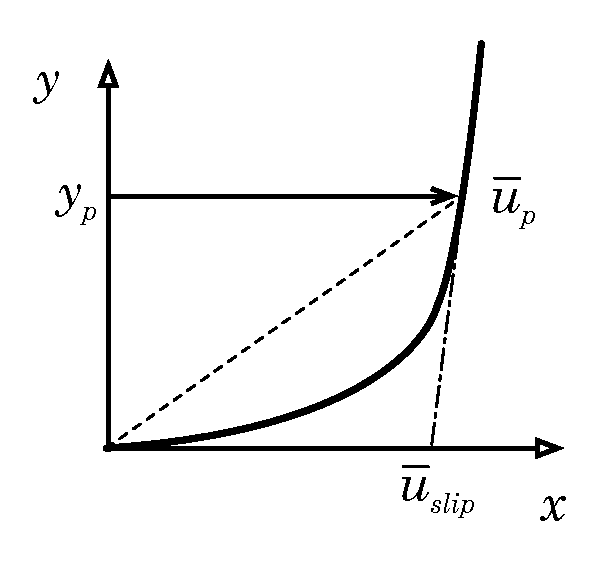
\includegraphics[width=5cm,clip]{wallfunc.eps}
\end{center}
\caption{壁面近傍の無次元速度プロファイル(\cite{kajishima:99:simulation}から転写)}
\label{fig:wall func}
\end{figure}


%%
\subsubsection{壁法則の適用}
%
\paragraph{発達した流れの場合}
チャネル流や円管内の発達流の場合,平均圧力勾配$\partial p^{\prime} / \partial x_i^{\prime}$と壁面摩擦力$\tau^{\prime}_w$が釣り合うので,\textbf{式(\ref{eq:friction velocity})}から摩擦速度がわかる.
第一格子点が対数則の範囲内であることが確認できれば,\textbf{式(\ref{eq:log-law log_e})}を利用できる.

%
\paragraph{流れの状況に応じて壁面摩擦が決まる場合}
一般的には,流れの様子により局所的な摩擦速度の大きさは異なるため,反復的に求める.
ある時点での$y_p^{\prime}$における$u_p^{\prime}$を与えて,関数として次の形を満たす$u_{\tau}^{\prime}$をニュートン反復により求める.

\begin{equation}
F(u_{\tau}^{\prime}) \,\equiv \, \frac{u_p^{\prime}}{u_{\tau}^{\prime}} - \frac{1}{\kappa}\mathrm{ln}\,\left( \frac{u_{\tau}^{\prime} \, y_p^{\prime}}{\nu} \right)\,-\,C \,=\,0
\label{eq:wall func newton}
\end{equation}

\noindent mを反復回数とすると,
\begin{equation}
{u_{\tau}^{\prime}}^{m+1} \,=\, {u_{\tau}^{\prime}}^{m} - \frac{F\left( {u_{\tau}^{\prime}}^{m} \right)}{F^{(1)} \left( {u_{\tau}^{\prime}}^{m} \right)}
\label{eq:newton iteration wall func}
\end{equation}

\noindent 対数則の場合には$F$の一階導関数は,
\begin{equation}
F^{(1)} \left( {u_{\tau}^{\prime}} \right) \,=\,
- \left( {\frac{u_p^{\prime}}{u_{\tau}^{\prime}} + \frac{1}{\kappa}} \right) \, \frac{1}{u_{\tau}^{\prime}}
\label{eq:derivative wall func}
\end{equation}

\noindent \textbf{式(\ref{eq:wall func newton})}$\sim$\textbf{(\ref{eq:derivative wall func})}から反復式を表すと,

\begin{equation} 
{u_{\tau}^{\prime}}^{\,m+1} \,=\, {u_{\tau}^{\prime}}^{\,m} + 
\frac{ 
\displaystyle{
\left\{
\frac{u_p^{\prime}}{{u_{\tau}^{\prime}}^{\,m}}
 - \frac{1}{\kappa} \, 
 \mathrm{ln}\,\left( \frac{y_p^{\prime} \, {u_{\tau}^{\prime}}^{\,m}} {\nu} \right) 
 \,-\, C \right\} \, 
 {u_{\tau}^{\prime}}^{\,m} }
}
{ \displaystyle{ \frac{u_p^{\prime}}{{u_{\tau}^{\prime}}^{\,m}} + \frac{1}{\kappa} }
}
\label{eq:newton iteration wall func}
\end{equation}


摩擦速度を無次元で表し$u_{\tau}\,=\,u_{\tau}^{\prime}/u_0^{\prime}$とすると,

\begin{equation} 
u_{\tau}^{\,m+1}
\, = \,
u_{\tau}^{\,m} + 
\frac{ 
\displaystyle{
\left\{ 
u_p^{+\,m} - \frac{1}{\kappa} \, 
 \mathrm{ln}\,\left( y_p^{+\,m} \right) \,-\, C \right\} \, u_{\tau}^{\,m} }
}
{ \displaystyle{ u_p^{+\,m} + \frac{1}{\kappa} }
}
\label{eq:newton iteration wall func ND}
\end{equation}

上記の手順により求めた$u_{\tau}^{\prime}$に対して,$y_p^{\prime}$が対数則の範囲にあるかどうかを判定し,壁法則を適用する.

%
\vspace{5mm}
\paragraph{摩擦速度求解のアルゴリズム}
与えられたセル近傍の速度から摩擦速度を求める手順は以下のようになる.

\begin{enumerate}
\item 反復の初期値を計算する.
\begin{equation}
\begin{array}{l}
\vspace{3mm}
\displaystyle{ \tau_w^0 \,=\, \frac{\tau_w^{\,\prime}}{\rho^{\prime} {u_0^{\prime}}^2} \,=\, \frac{1}{Re} \frac{\partial u}{\partial y} }\\
\vspace{3mm}
\displaystyle{ u_{\tau}^{\,0} \,=\, \frac{u_{\tau}^{\prime\,0}}{u_0^{\prime}} \,=\, \frac{1}{u_0^{\prime}} \sqrt{\frac{\tau_w^{\,\prime}}{\rho^{\prime}}}
\,=\, \sqrt{\frac{1}{Re} \frac{\partial u}{\partial y}} }\\
\vspace{3mm}
\displaystyle{ {y_p^+}^{\,0} \,=\, \frac{u_{\tau}^{\,0} \, u_0^{\prime} \, y_p^{\prime} }{\nu} }
\,=\, u_{\tau}^{\,0} \, y_p^{\prime} \, \frac{Re}{L^{\prime}}\\
\end{array}
\label{eq:initial iteration fric vel}
\end{equation}
ここで,$L^{\prime}$は代表長さ,$y_p^{\prime}=h^{\prime}/2$(バイナリボクセルの場合は,壁面から半セルの距離)である.
速度勾配は次の2つの候補がある.
\vspace{1mm}

\begin{indentation}{5zw}{0zw}

\begin{enumerate}
\item 壁面から半セルの距離にある速度定義点の速度の大きさで評価
\begin{equation}
\frac{\partial u}{\partial y}  \,=\, \frac{\Delta u}{\Delta y} \,=\, \frac{|u|}{h/2}
\label{eq:vel mag wall func}
\end{equation}

\item \textbf{図\ref{fig:wall func}}の$y_p$の位置での速度勾配を壁関数\textbf{(\ref{eq:log-law log_10})}から求める
\begin{equation}
\frac{\partial u}{\partial y}  \,=\, \frac{5.75}{y_p^+ \, \mathrm{ln}10}
\label{eq:dudy wall func}
\end{equation}

\end{enumerate}

\end{indentation}

\vspace{2mm}

\item Newton反復(常用対数を用いて)
\begin{equation} 
u_{\tau}^{\,m+1} \,=\, u_{\tau}^{\,m} + 
\frac{ \displaystyle{
\left\{ u_p^{+\,m} -  5.75 \, \mathrm{log_{10}}\,{y_p^+}^m \,-\, 5.5 \right\} \, u_{\tau}^{\,m} }
}{ \displaystyle{
u_p^{+\,m} + \frac{1}{\kappa} }
}
\label{eq:newton iteration wall func ND2}
\end{equation}

\vspace{2mm}
\item 収束判定
次式により収束判定を行う.
\begin{equation} 
\displaystyle{ \frac{|u_{\tau}^{\,m+1}-u_{\tau}^{\,m}|}{|u_{\tau}^{\,m}|} < \epsilon_2 \quad(=10^{-3}) }
\label{eq:newton iteration criteria}
\end{equation}

ここで,$u_{\tau}^{\,m+1}<\epsilon_2$の場合には,安定性のために$u_{\tau}^{\,m+1}=\epsilon_2$とする.
\vspace{2mm}

\item 更新\\
\begin{equation}
\begin{array}{l}
u_{\tau}^{\,m} \,=\, u_{\tau}^{\,m+1}\\
\vspace{2mm}
\displaystyle{ {y_p^+}^{\,m} \,=\, u_{\tau}^{\,m+1} \, y_p^{\prime} \, \frac{Re}{L^{\prime}} }\\
\end{array}
\label{eq:newton iteration wall func ND2}
\end{equation}
\vspace{2mm}

\item 上記を収束するまで繰り返す.反復上限を10回程度で抑えておく.
\end{enumerate}


%
\subsubsection{減衰関数を用いたすべりなし条件}

壁近傍ではGSで速度勾配があるため,SGS応力が生じる.しかし,壁面上では$\tau_{ij}=0$なので,これを打ち消す必要がある.
Smagorinskyモデルでは減衰関数$f_s$を導入し,渦粘性係数を補正する.

\begin{equation}
\nu_e \,=\, \left( Cs \,f_s \, \overline{\Delta} \right)^2 \left| \overline{D} \right|
\label{eq:nu-SGS modified}
\end{equation}

\noindent 減衰関数としてはvan Driest関数を用いる.

\begin{equation}
f_s \,=\, 1 - \mathrm{exp} \left( -\frac{y^+}{A^+} \right)
\label{eq:van-driest}
\end{equation}

\noindent $A^+$は無次元の定数で約25が用いられる.

すべりなし条件を用いる場合には,粘性底層からバッファ層にかけて,格子点が数点必要である.
この場合,粘性底層内では乱流応力は無視できるので,壁面摩擦応力$\tau_w^{\prime}$は次のように決められる.

\begin{equation}
\tau_w^{\prime} \,=\, \mu \left| \frac{\partial \overline{u^{\prime}}}{\partial y^{\prime}} \right|_{wall}
\label{eq:viscous layer stress}
\end{equation}

%
\subsection{壁法則から求めた壁面摩擦応力による粘性応力の置換}
壁面に接する流体セルの固体セルへの接平面上の壁面摩擦応力$\tau_w^{\prime}=\mu(\partial u^{\prime}/\partial y^{\prime})$は壁法則\textbf{(\ref{eq:friction velocity})}から求められる摩擦速度から$\tau_w^{\prime}\,=\, \rho^{\prime} {u_{\tau}^{\prime}}^2$として計算される.この壁面摩擦応力を粘性項の離散式に代入し境界条件とする.たとえば,z軸のマイナス方向に壁面がある場合,無次元形式で,

\begin{equation}
\frac{1}{Re} \frac{\partial}{\partial z} \left( \frac{\partial u}{\partial z} \right)
\,=\,
\frac{1}{h} \, \left( {\frac{1}{Re} \frac{\partial u}{\partial z}_t - \tau_{w,\,b} } \right)
\label{eq:replace wall shear stress}
\end{equation}


計算された摩擦速度から壁面摩擦応力を計算し,\textbf{式(\ref{eq:replace wall shear stress})}により境界条件を与える.固体セルに隣接する流体セルにおいて摩擦速度が求まると,固体に接する面上の応力は次式により計算される.

\begin{equation} 
\tau_w\,=\, u_{\tau}^2
\label{eq:wall stress from fric vel}
\end{equation}

\noindent しかしながら,複数の固体面に接するセルでは各方向同じ大きさの壁面摩擦応力となるし,軸方向に沿わない速度ベクトルの場合には過大評価になる可能性がある.そこで,速度ベクトルの方向成分を計算し,各方向へ射影する.つまり,\textbf{式(\ref{eq:wall stress from fric vel})}に用いる$u_{\tau}$を再定義する.

\begin{equation} 
\tau_{w,\,i} \,=\, {\left( u_{\tau} \frac{u_i}{|u|} \right)}^2
\label{eq:redefine of friction velocity}
\end{equation}







%%%
\chapter{解析モデルの作成}

\begin{abstract}
この章では,解析モデルの作成方法を説明します.解析モデルの作成については,Fxgenアプリケーションを用いて,ポリゴンにラベルと境界条件タグを付与します.また,形状データが不要な組み込み例題について説明します.
\end{abstract}
%

\graphicspath{{./fig_Model/}}

%
\section{形状近似度による解析モデルの分類}
\label{sec:classification of model}
直交格子を用いる流体解析では,解析対象となる形状を直交格子上でどのように扱うかにより,計算のロバスト性,予測精度,計算時間,計算格子(解析モデル)の作りやすさなどの特性が異なります.一般には,\textbf{図\ref{fig:class model}}のように分類することができます\cite{CFDハンドブック:03}.

\begin{figure}[htdp]
\begin{center}
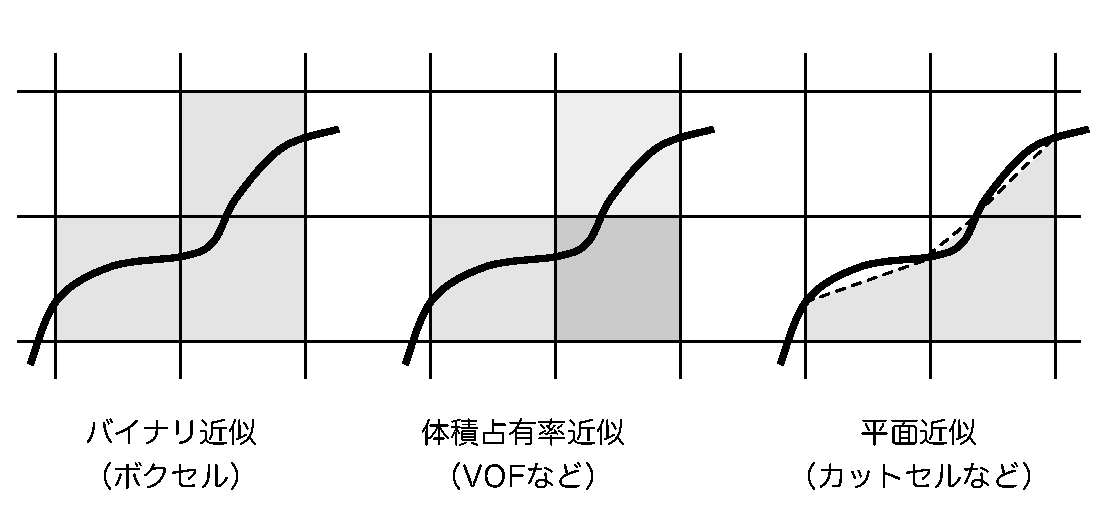
\includegraphics[width=11cm,clip]{classification.eps}
\caption{直交格子における形状近似度の分類}
\label{fig:class model}
\end{center}
\end{figure}

%
\subsection{Binary Voxel}
\label{sec:binary voxel}
Binary Voxel\index{Binary Voxel}モデルは,\textbf{図\ref{fig:Eport binary voxel}}に示すように立方体のセル要素単位で形状を表現する解析モデルです.
物体の形状近似としては最も簡単であり,モデル作成時のロバスト性に大きな利点があります.

\begin{figure}[htbp]
\begin{minipage}{.6\textwidth}
\begin{center}
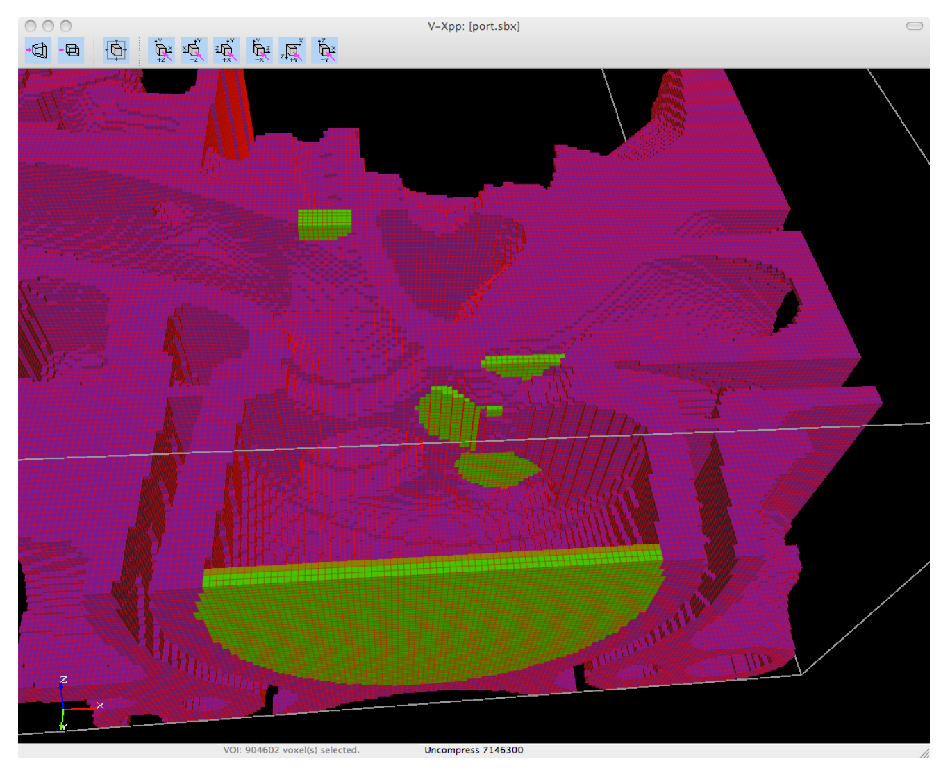
\includegraphics[width=8cm,clip]{eport.eps}
\end{center}
\caption{バイナリボクセルによる機械部品の形状表現とセルID設定}
\label{fig:Eport binary voxel}
\end{minipage} \hfill
\begin{minipage}{.38\textwidth}
\begin{center}
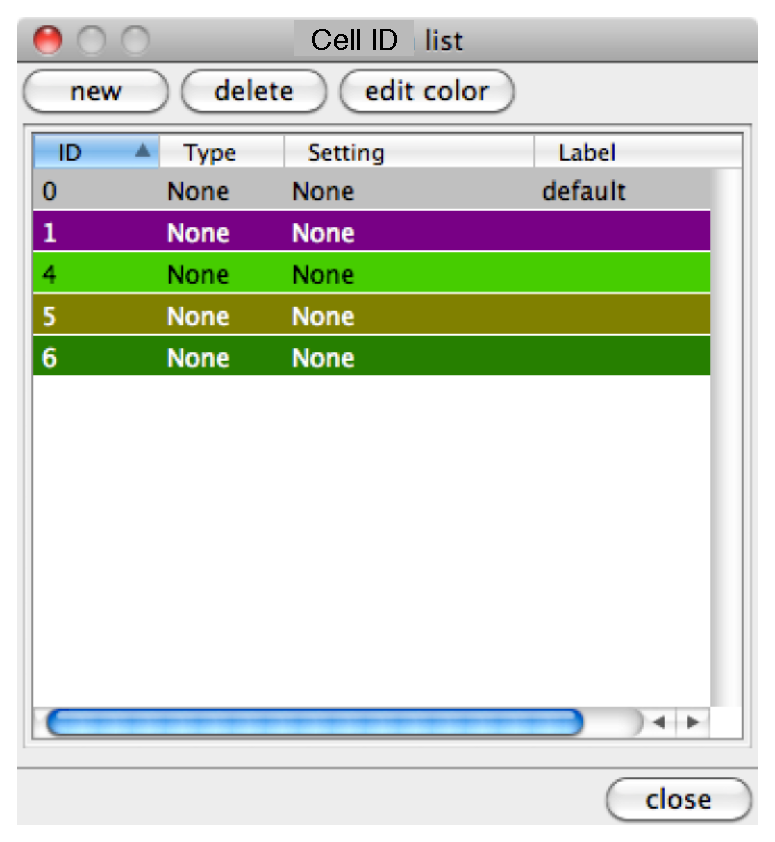
\includegraphics[width=6cm,clip]{Mlist.eps}
\end{center}
\caption{V-XgenでのセルID設定リスト}
\label{fig:ID set on V-Xgen}
\end{minipage}
\end{figure}

%
\subsection{体積率モデル}
Binary Voxelの形状近似度を改善する方法の一つで,セル内における流体の占有率を考慮した計算をする場合に利用します.
陽的な面の情報をもたないので,界面は拡散的に表現される傾向です.補助的に面における開口率を用いる場合には,有限体積法との親和性が高く保存性が改善されます.
%
\subsection{カットモデル}
\label{sec:planar cut}
Binary Voxelでは形状が階段状に近似されるため,計算精度が不足する場合があります.そこで,形状を区分的にカットされた平面として近似するモデルを用います.
CPCソルバー\footnote{\today 未実装.}では,物理量の定義点から物体までの距離情報を用いることにより,ロバスト性と精度向上の両立を図っています.通常のボクセルについてはバイナリボクセルと同様です.


%
\section{セルIDによる境界条件の指定}
\label{sec:ID connection}

CBC/CPCソルバーでは,ボクセルの各セルにIDを与え,このセルIDとパラメータファイルに記述された境界条件情報から,境界条件を設定するしくみになっています.
例えば,ボクセルモデルのセルIDとXML記述のパラメータファイル中では,次のように媒質IDと結びつけられます.

{\small
\begin{program}
<Elem name="Model_Setting">
  <Param name="fluid" id="1"   dtype="INT" value="100" comment="air"/>
  <Param name="solid" id="600" dtype="INT" value="600" comment="wall"/>
  <Param name="solid" id="610" dtype="INT" value="600" comment="piston_head"/>
</Elem>
\end{program}
}

\noindent ここでは,流体であるセルID=1は媒質ID=100によりその物性値が定義され,airのコメントがつけられています.
参照される媒質IDは,Medium\_Tableタグによって次のように指定されます.

{\small
\begin{program}
<Medium_Table>
  <Elem name="Fluid" id="100" comment="Air">
    <Param name="density"              dtype="REAL" value="1.1763" />
    <Param name="specific_heat"        dtype="REAL" value="1007" />
    <Param name="thermal_conductivity" dtype="REAL" value="2.614e-02" />
    <Param name="kinematic_viscosity"  dtype="REAL" value="15.83e-06" />
    <Param name="viscosity"            dtype="REAL" value="18.62e-06" />
    <Param name="sound_of_speed"       dtype="REAL" value="340.0" />
  </Elem>
  <Elem name="Solid" id="600" comment="Fe">
    <Param name="density"              dtype="REAL" value="7870.0" />
    <Param name="specific_heat"        dtype="REAL" value="442.0" />
    <Param name="thermal_conductivity" dtype="REAL" value="80.3" />
  </Elem>
</Medium_Table>
\end{program}
}

媒質IDの指定についての詳細は,\hyperlink{tgt:medium_table}{Medium\_Table}セクションを参照してください.

\pagebreak
%
\section{形状データからの解析モデルの作成手順}
\label{sec:modeling procedure}
V-Xgen\index{V-Xgen}を用いた解析モデル作成の手順を簡単に示します.操作の詳細は,V-Xgenユーザーガイド,およびチュートリアルを参照してください.

\begin{enumerate}
\item V-Xgenの起動\\
アイコンのダブルクリック,または下記のようにコマンドラインからアプリケーションを起動します.

{\small
\begin{program}
$ Vxgen.sh または Vxgen
\end{program}
}

\item ファイルの読み込み\\
入力となる幾何形状STLファイル\index{STL}を読み込みます.
\verb|File > Import > Shape (obj/stl) data files...|のコマンドを実行し,ファイルリストから幾何形状ファイルを選択しロードすると,\textbf{図\ref{fig:V-Xgen mesh}}のように形状モデルが描画されます.\\

\begin{figure}[htbp]
\begin{minipage}{.6\textwidth}
\begin{center}
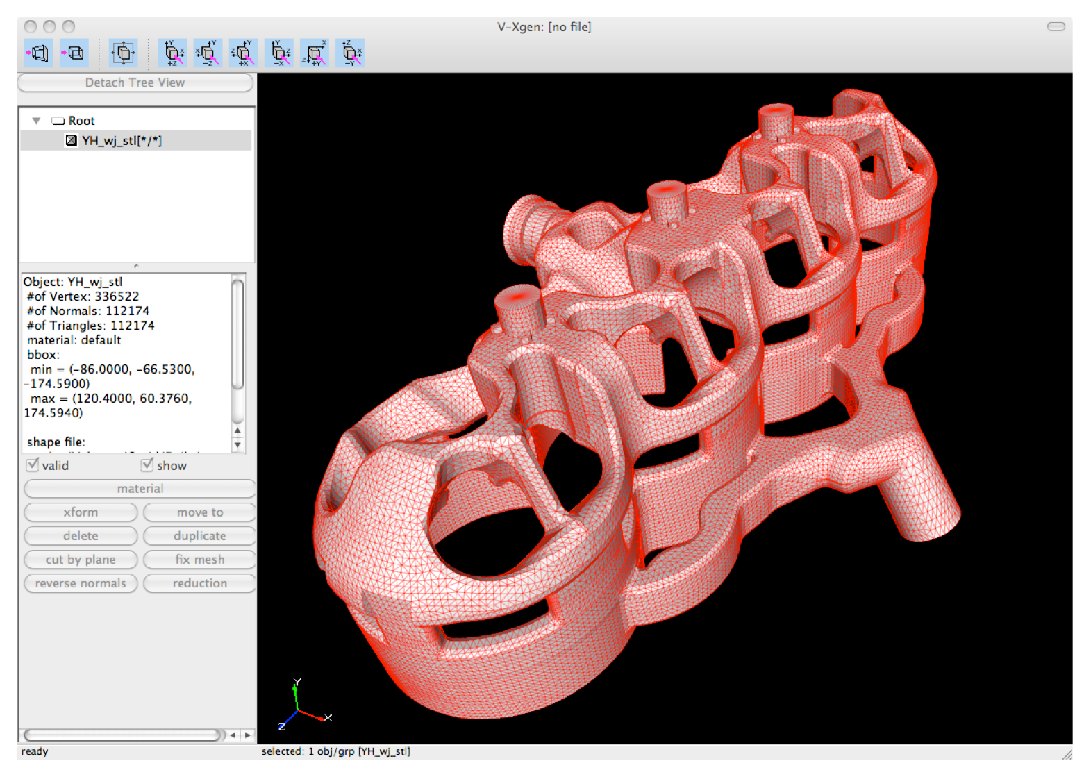
\includegraphics[width=8.5cm,clip]{WJ_mesh.eps}
\end{center}
\caption{V-Xgenでのファイル読み込み}
\label{fig:V-Xgen mesh}
\end{minipage} \hfill
\begin{minipage}{.38\textwidth}
\begin{center}
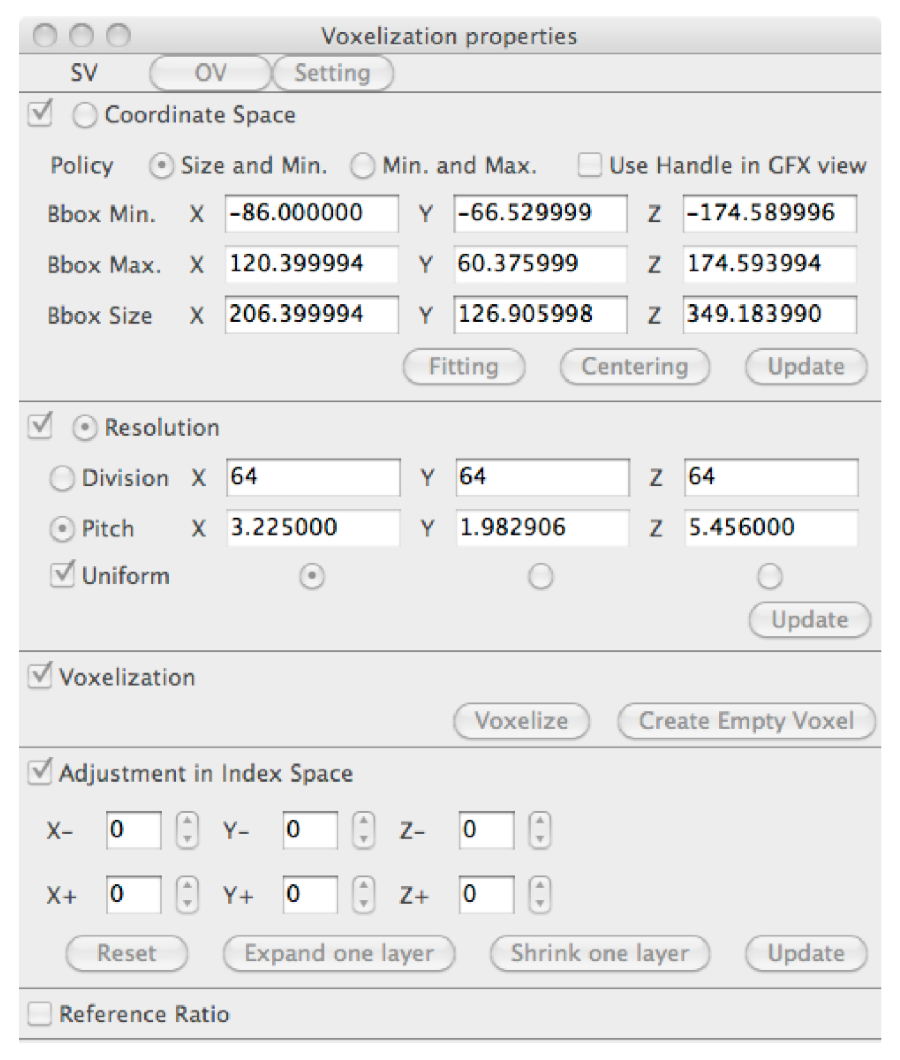
\includegraphics[width=6cm,clip]{SV_dialog.eps}
\end{center}
\caption{ボクセル作成のパラメータ設定ダイアログ}
\label{fig:SV menue}
\end{minipage}
\end{figure}

\item バイナリボクセルの作成\\
\verb|Voxelization > Simple Voxel(SV) ...|を実行すると,\textbf{図\ref{fig:SV menue}}のような直交等間隔ボクセルを作成するダイアログが表示されます.
パラメータを適切に設定して,ボクセルを作成すると,\textbf{図\ref{fig:V-Xgen voxelize}}のようなボクセルのバウンディングボックスが表示されます.
ここで作成するボクセルモデルの範囲は,\textbf{図\ref{fig:cal. region}}に示す計算領域の部分です.
計算に必要な計算領域の外部に位置する仮想セル領域の媒質はXMLパラメータファイルのOuterBoundary$\to$Face\_BC中のCell\_IDタグで指定します.\\

\begin{figure}[htbp]
\begin{minipage}{.48\textwidth}
\begin{center}
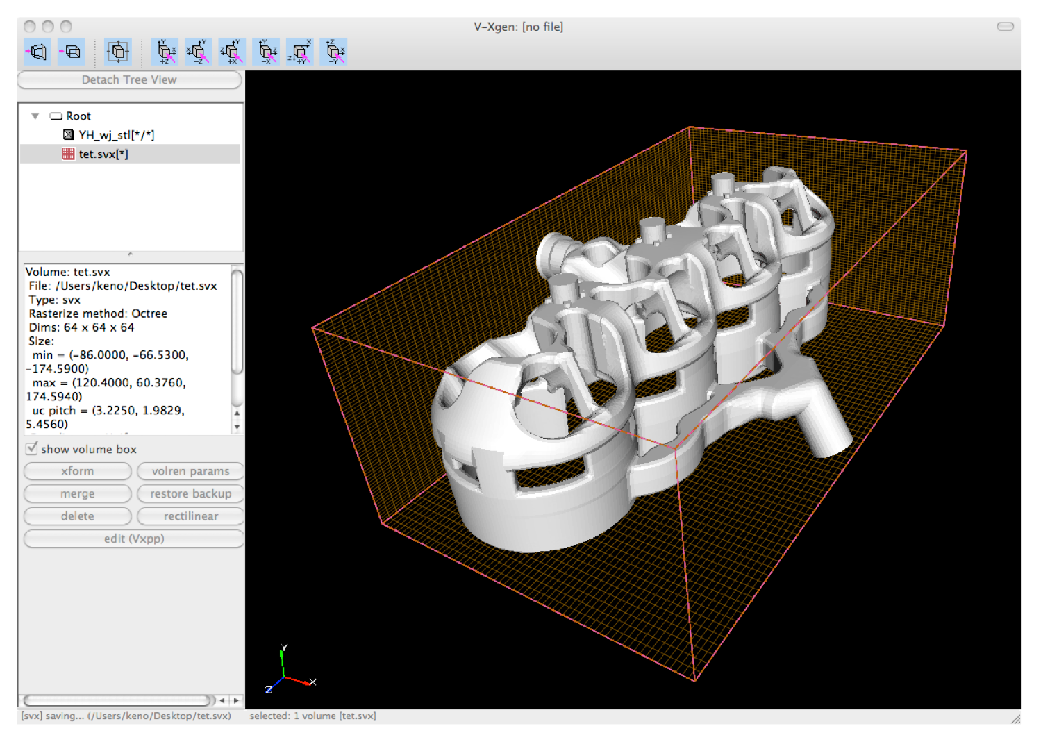
\includegraphics[width=8cm,clip]{voxelize.eps}
\end{center}
\caption{V-Xgenでのボクセル生成}
\label{fig:V-Xgen voxelize}
\end{minipage} \hfill
\begin{minipage}{.48\textwidth}
\begin{center}
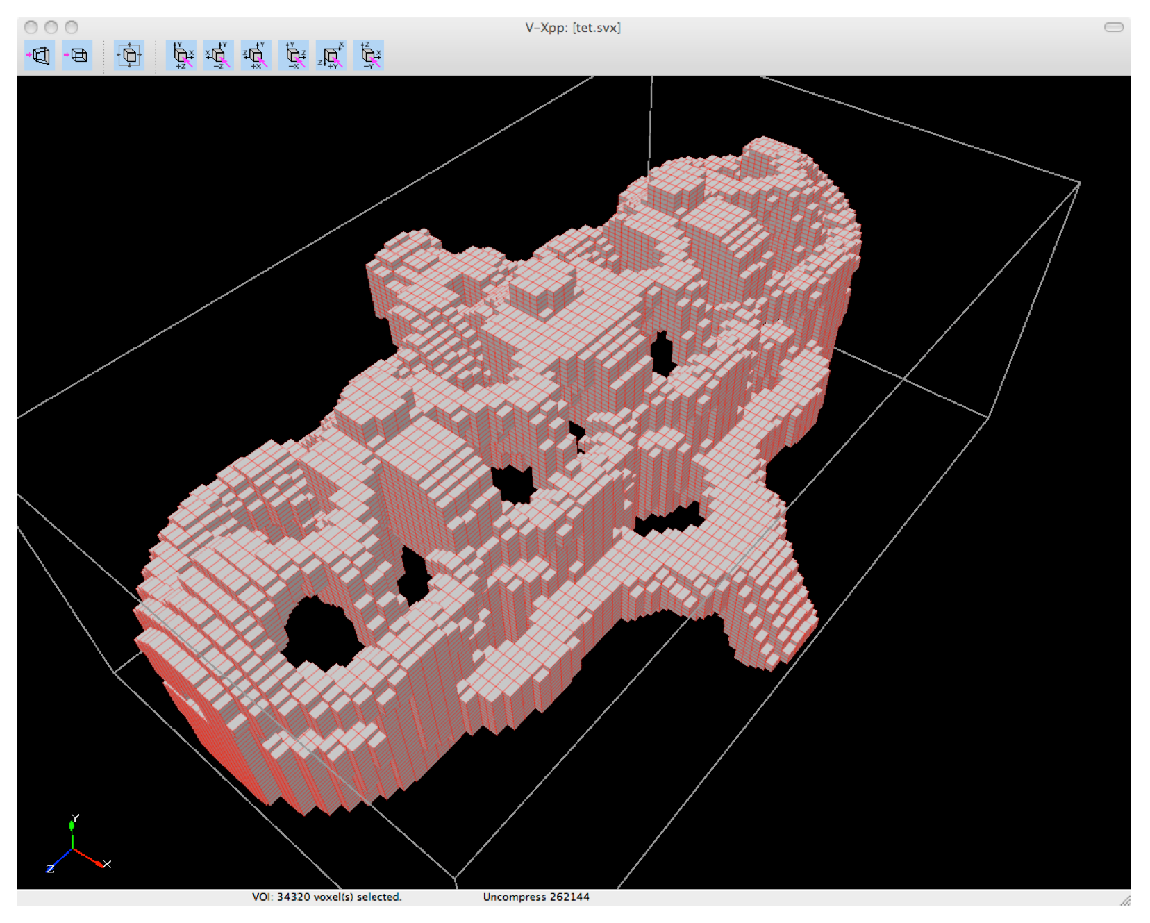
\includegraphics[width=7cm,clip]{WJ_voxel.eps}
\end{center}
\caption{ボクセルモデル.V-XppのVOIコマンドによる選択状態の表示}
\label{fig:V-Xpp voxel}
\end{minipage}
\end{figure}

\begin{figure}[htdp]
\begin{center}
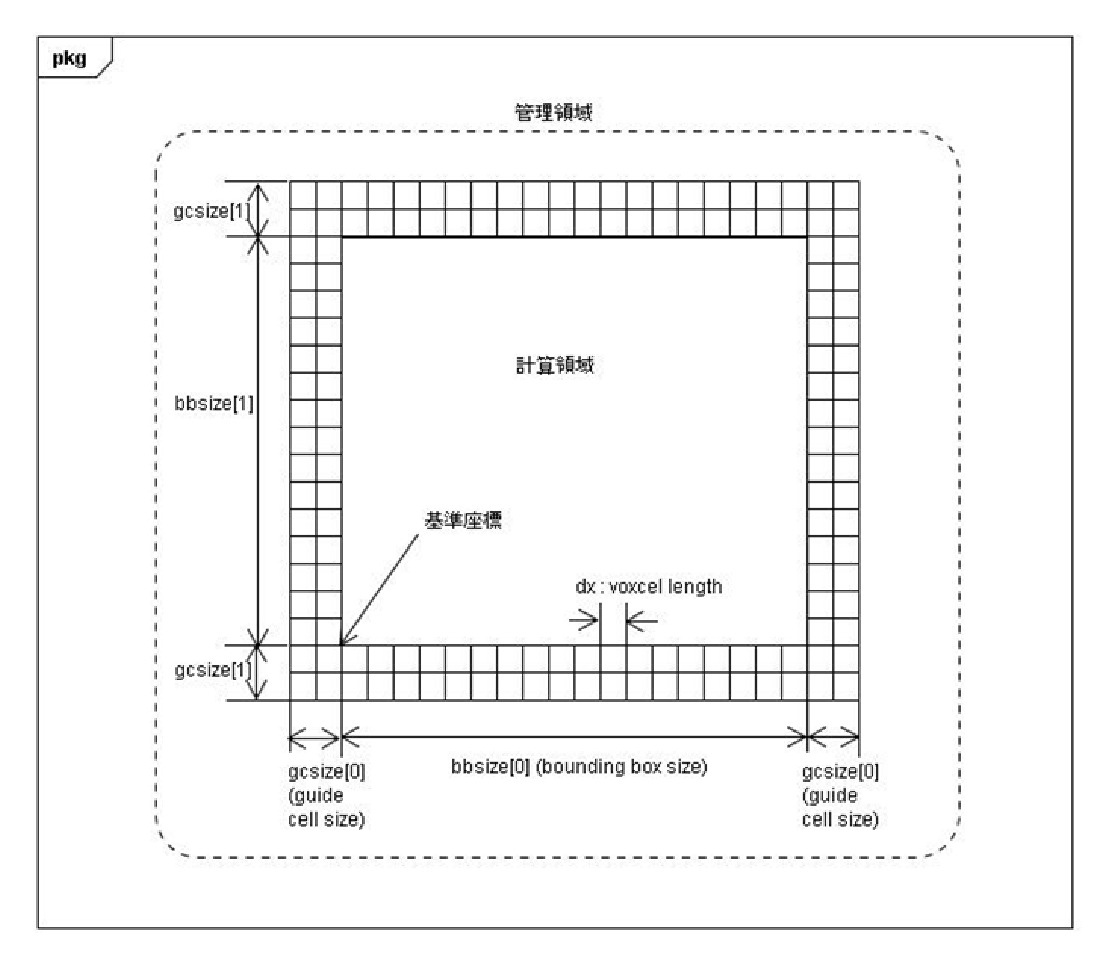
\includegraphics[width=12cm,clip]{clip006.eps}
\caption{計算領域とガイドセル領域の定義}
\label{fig:cal. region}
\end{center}
\end{figure}


\item セルIDの設定\\
V-Xgenで作成したボクセルモデルファイルを,アプリケーションV-Xpp\index{V-Xpp}を用いてセルIDを編集します\footnote{次のバージョンでは,V-Xppの機能をV-Xgenに統合予定です.}.V-Xppを起動し,\verb|File > Open...|を実行してボクセルモデルファイル(*.svx, *.sbx, *.ovx)を選択しロードすると,\textbf{図\ref{fig:V-Xpp voxel}}のようにボクセライズされた形状データが表示されます.\\

 次に,\verb|Volume > Medium List...|を選択し,\textbf{図\ref{fig:V-Xpp Medium list}}に示すセルIDリストを編集します.
ボクセルモデルを\verb|VOI > Select VOI...|や\verb|VOI > Slice Control...|によりボクセルを選択,\verb|VOI > Set Cell ID...|コマンド(\textbf{図\ref{fig:V-Xpp set cell ID}})によりセルIDを選択対象セルに設定します.
セルIDを編集したボクセルモデルは\textbf{図\ref{fig:editted voxel}}のようになるのでファイルに保存します.
ここで,約束事として,\textbf{セルID=0は予約番号でユーザは設定しないこと}に注意してください.\\

また,利用できるIDの設定数に関しては,\hyperlink{tgt:localboundary}{LocalBoundary}で説明していますが,\textbf{指定できる内部境界条件の数は30個が上限で,かつ指定境界条件数と媒質数の和は63個以下}となる点に注意してください.

\begin{figure}[htbp]
\begin{minipage}{.48\textwidth}
\begin{center}
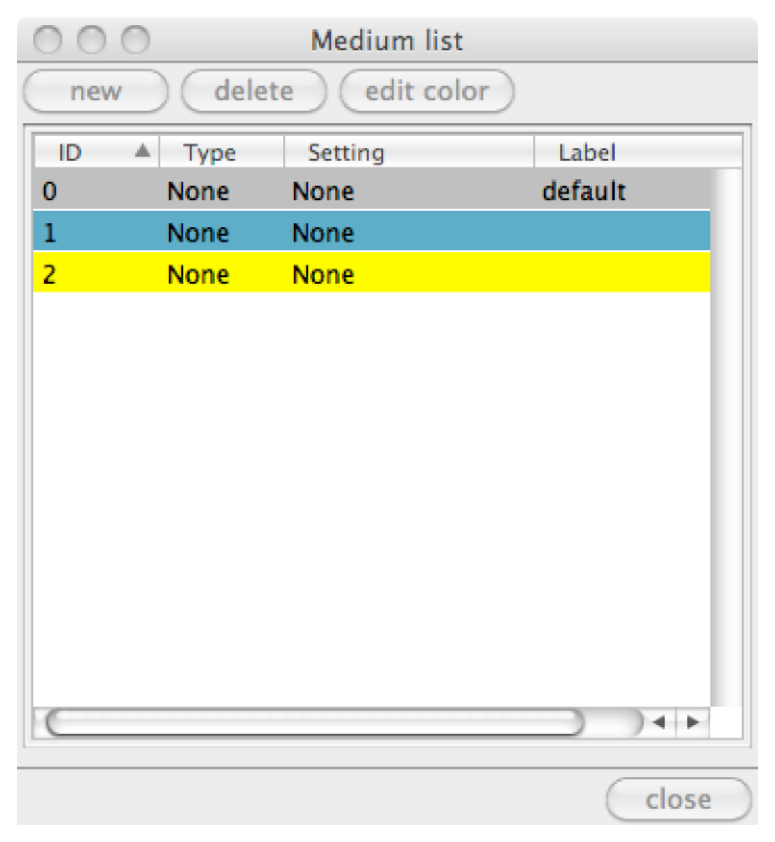
\includegraphics[width=6cm,clip]{VXpp_Mlist.eps}
\end{center}
\caption{セルID編集ダイアログ}
\label{fig:V-Xpp Medium list}
\end{minipage} \hfill
\begin{minipage}{.48\textwidth}
\begin{center}
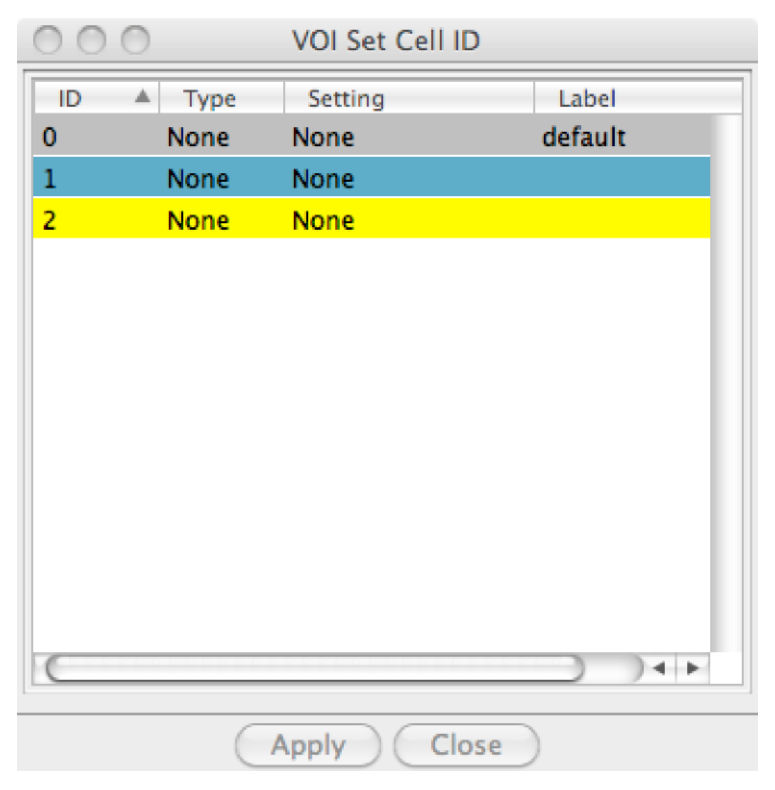
\includegraphics[width=6cm,clip]{VXpp_setID.eps}
\end{center}
\caption{セルID設定ダイアログ}
\label{fig:V-Xpp set cell ID}
\end{minipage}
\end{figure}

\begin{figure}[htdp]
\begin{center}
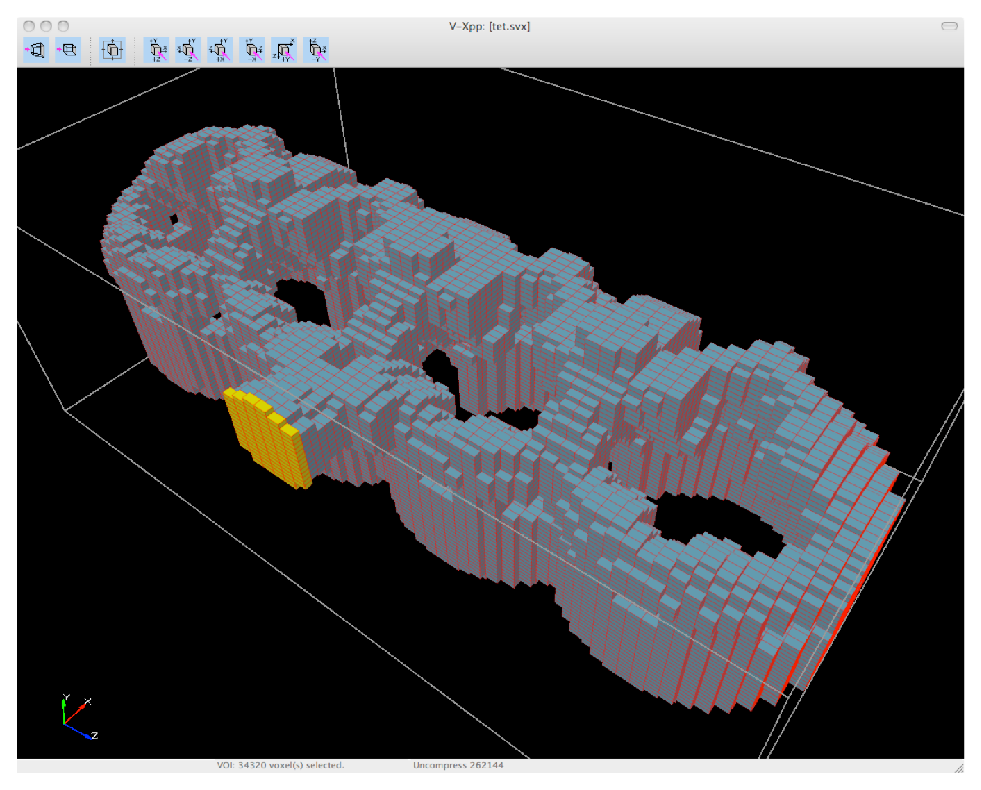
\includegraphics[width=12cm,clip]{VXpp_coloredVoxel.eps}
\caption{V-XppでセルIDを編集したボクセルモデル}
\label{fig:editted voxel}
\end{center}
\end{figure}

\end{enumerate}

\pagebreak


%% 
\section{組み込み例題}
\hypertarget{tgt:intrinsic model}{組み込み例題}は,FFV-Cソルバーに組み込み済みの解析モデルです.
プログラムに組み込まれた解析モデルを用いることにより,解析モデルを作成しなくても計算ができます.
ただし,\textbf{表\ref{tbl:intrinsic problems}}に示すような簡単な形状のモデルに限られます.
各モデルに固有のパラメータは,Parameter $>$ Intrinsic\_Exampleセクションで指定します.

\begin{table}[htdp]
\caption{組み込み例題クラス}
\begin{center}
\small
\begin{tabular}{lll}\toprule
組み込みモデル名 & 利用クラス & 説明\\ \midrule
%Users & IP\_Users & ユーザ問題(解析モデルファイルを指定する場合)\\ \hline
%Back\_Step & IP\_STEP & バックステップ流れのモデル\\
%Cylinder & IP\_CYLINDER & 角柱と円柱周りの流れのモデル\\
%Duct & IP\_Duct & 円形と正方形のダクト流れのモデル\\
%Parallel\_Plate\_2D & IP\_PPLT2D & 二次元平行平板のモデル(Poiseuille流れ,Couette流れなど)\\
Performance\_Test & IP\_PMT & 性能測定を行うためのモデル(三次元立方体キャビティフローと同じ問題設定)\\
%Polygon & IP\_Polygon & 距離情報スキームを用いる場合に,入力するポリゴンファイル名とDomainInfoの\\
% & & 指定だけで計算するモデル\\
Rectangular & IP\_Rect & 計算領域が矩形で,かつ単一媒質のモデル\\
%SHC1D & IP\_SHC1D & 一次元の熱伝導問題のモデル\\ 
\bottomrule
\end{tabular}
\end{center}
\label{tbl:intrinsic problems}
\end{table}

%
\begin{comment}
\subsection{IP\_STEPクラス}
バックステップ流れを計算するクラスです.
\textbf{図\ref{fig:ip_backstep}}と\textbf{表\ref{tbl:ip_backstep}}および\textbf{表\ref{tbl:ip_backstep_ID}}に示すパラメータで計算空間を構成します.
計算領域は,Domain\_Infoで指定するVoxelSize,VoxelPitch,VoxelOriginで決まります.

ドライバー部分については,Ductクラスの設定を参照してください.

\begin{figure}[htdp]
\begin{center}
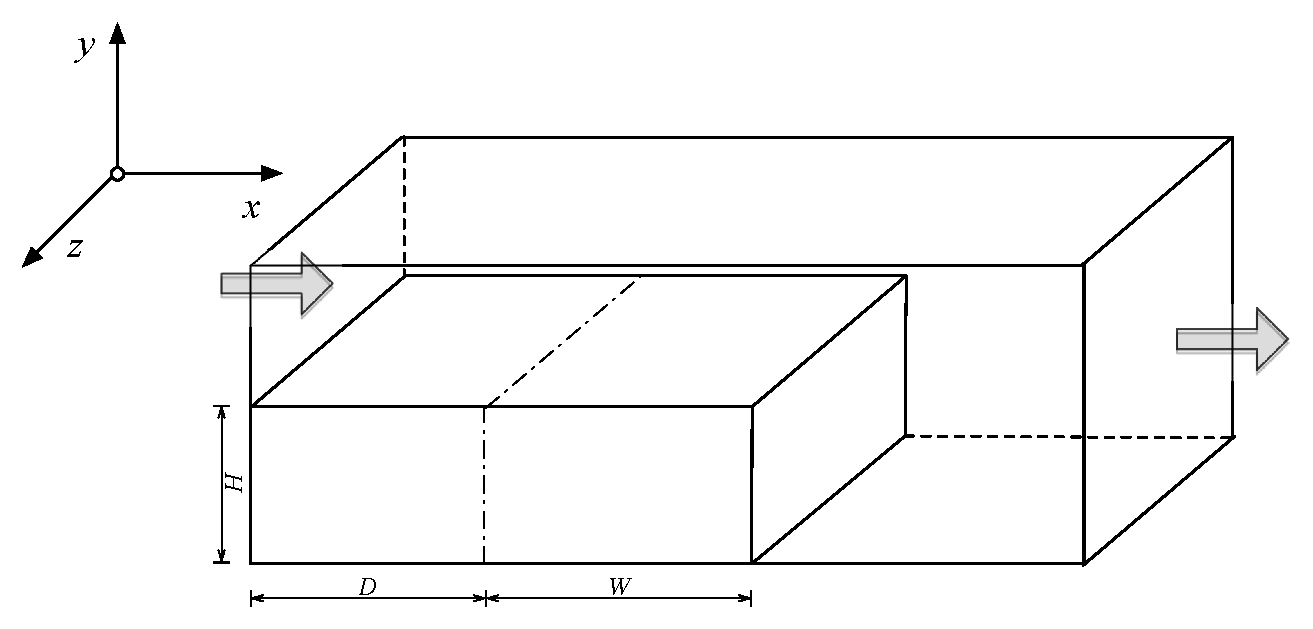
\includegraphics[width=14cm,clip]{Backstep.eps}
\end{center}
\caption{バックステップ流れの計算モデル.}
\label{fig:ip_backstep}
\end{figure}

\begin{table}[htdp]
\small
\caption{バックステップ問題のパラメータ.}
\begin{center}
\begin{tabular}{ll}\toprule
記号 & パラメータ\\ \midrule
Mode & 2D $|$ 3D\\ \hline
Width ($W$) & ステップの$x$方向の幅\\
Height ($H$) & ステップの$y$方向の高さ\\
Driver ($D$) & ドライバー部分の長さ($>0.0$でドライバあり,=0.0の場合ドライバーなし)\\
\bottomrule
\end{tabular}
\end{center}
\label{tbl:ip_backstep}
\end{table}

\begin{table}[htdp]
\small
\caption{バックステップ問題のID番号.}
\begin{center}
\begin{tabular}{ll}\toprule
ID & 属性\\ \midrule
1 & 流体\\
2 & 固体\\
3 & ドライバ部分の流体\\
4 & ドライバ流出面(流体)\\
\bottomrule
\end{tabular}
\end{center}
\label{tbl:ip_backstep_ID}
\end{table}

境界条件として,X-方向に流入,またはドライバ境界,X+方向は流出条件,Y-方向は壁面,Y+方向は壁面またはスリップ条件,Z$\pm$方向は壁面か周期境界を与えて計算します.二次元の問題を解く場合には,Mode=2Dを指定,VoxelSizeはkmax=3として,Z方向は周期境界条件を与えてください.
\end{comment}

%
\begin{comment}
\subsection{IP\_CYLINDERクラス}
二次元と三次元の円柱・角柱まわりの流れを計算するクラスです.
\textbf{図\ref{fig:ip_cylinder}}と\textbf{表\ref{tbl:ip_cylinder}}に示すパラメータで計算空間を構成します.
断面形状は,円柱と角柱をShapeで指定します.それぞれの断面形状で指定するパラメータが異なります.
柱は$xy$平面の$z-$方向に接しています.これを基準に長さのパラメータを指定してください.

二次元の問題を解く場合には,Mode=2Dを指定,VoxelSizeはkmax=3としてください.この場合,パラメータ$W$は無視されます.

\begin{figure}[htdp]
\begin{center}
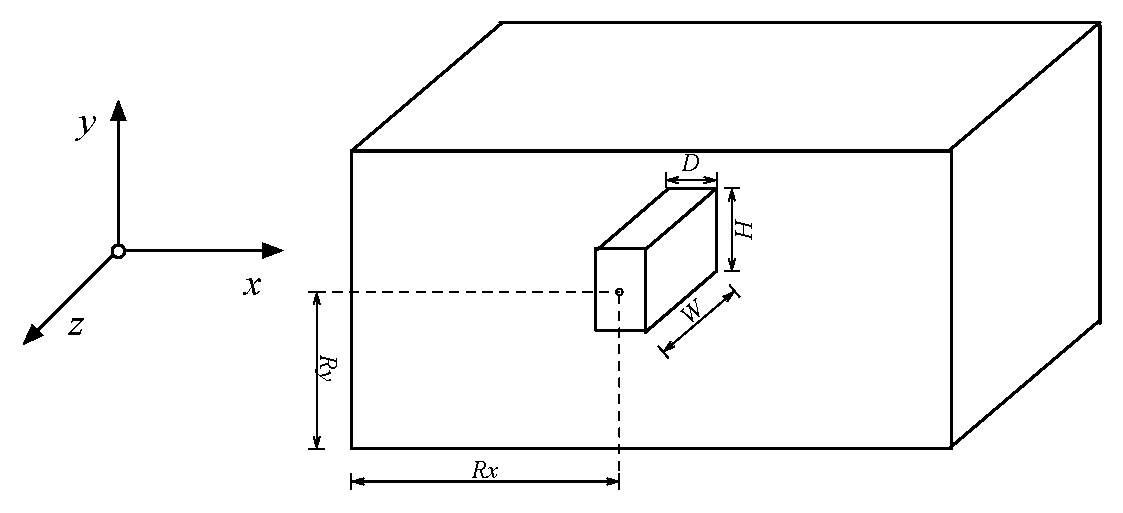
\includegraphics[width=14cm,clip]{Cylinder.eps}
\end{center}
\caption{円柱・角柱モデルの計算空間.}
\label{fig:ip_cylinder}
\end{figure}

\begin{table}[htdp]
\small
\caption{柱状物体の指定パラメータ}
\begin{center}
\begin{tabular}{ll}\toprule
記号 & パラメータ\\ \midrule
Mode & 2D $|$ 3D\\ 
Shape & Rectangular $|$ Circular\\ \hline
$D$ & 角柱を指定時の角柱の幅\\
$H$ & 角柱を指定時の角柱の高さ\\
$R$ & 円柱を指定時の半径\\
$W$ & 柱の$z$軸方向の長さ\\
$R_x$ & 柱の中心位置と$x$方向領域境界からの距離\\
$R_y$ & 柱の中心位置と$y$方向領域境界からの距離\\
\bottomrule
\end{tabular}
\end{center}
\label{tbl:ip_cylinder}
\end{table}
\end{comment}

%
\begin{comment}
\subsection{IP\_Ductクラス}
\textbf{図\ref{fig:ip_duct}}のような円形と矩形のダクト流れを計算するモデルで,周期境界条件を用います.
流入面には,流れを発達させる機能をもつドライバー部分を指定することができます.

断面形状は,正方形または円形をShapeで指定し,
流入部の方向をDirectionで指定します.
ドライバー部は,Directionで指定した方向にドライバ部分が配置されます.
ドライバー部分を指定する場合には,Driverにその長さ$D$を指定してください.
$D=0.0$の場合には,ドライバー無しの指定になります.

\begin{figure}[htdp]
\begin{center}
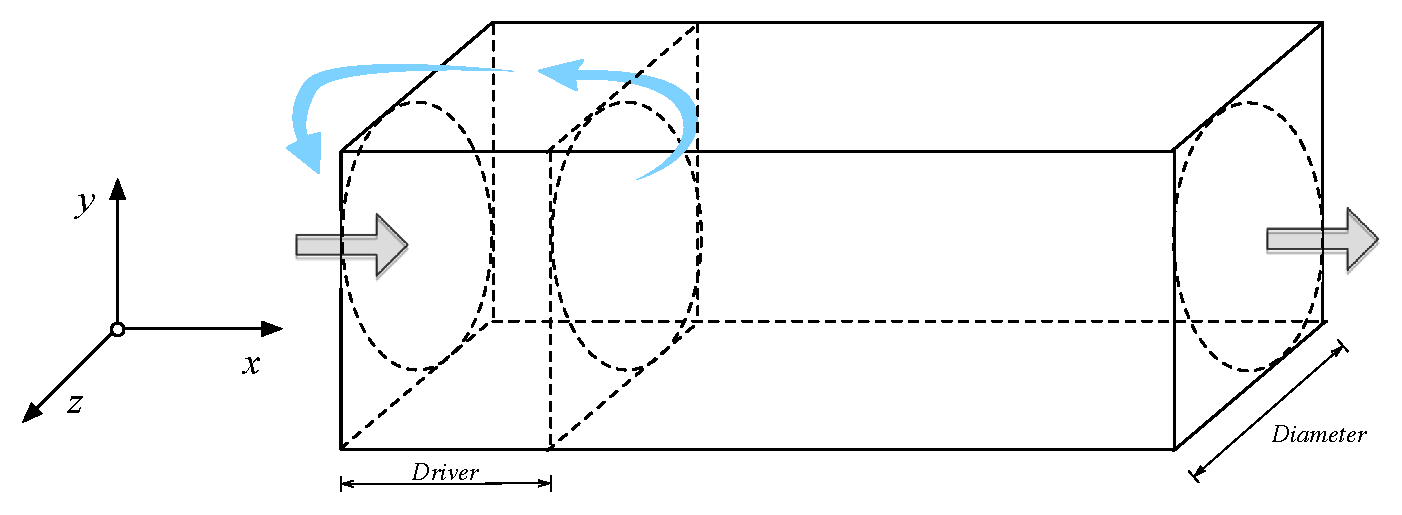
\includegraphics[width=16cm,clip]{Duct.eps}
\end{center}
\caption{ダクトの計算空間.$X-$方向にドライバ部を設置した場合.}
\label{fig:ip_duct}
\end{figure}

\begin{table}[htdp]
\small
\caption{ダクトの指定パラメータ}
\begin{center}
\begin{tabular}{ll}\toprule
記号 & パラメータ\\ \midrule
Shape & Rectangular $|$ Circular\\ \hline
Diameter & 正方形または円の直径\\
Direction & 周期境界と流入の方向(X\_minus, X\_plus, Y\_minus, Y\_plus, Z\_minus, Z\_plus)\\
Driver & ドライバー部分の長さ($>0.0$でドライバあり,=0.0の場合ドライバーなし)\\
\bottomrule
\end{tabular}
\end{center}
\label{tbl:ip_duct}
\end{table}
\end{comment}


%%
\subsection{IP\_PMTクラス}
FFV-Cソルバーの基本的性能を測定するための例題クラスです.
三次元立方体の空間内のキャビティフローを解きます.
性能測定モードとなり,圧力反復の収束判定は行わず,反復回数は固定となります.
また,初期化時のファイル出力が抑制されます.



%%
\begin{comment}
\subsection{IP\_PPLT2Dクラス}
二次元の平行平板間の流れを計算するためのクラスです.
\textbf{図\ref{fig:pplate2d}}のように辺長比が2:1の二次元空間を表現します.
z方向には3セルを設けており,単純な周期境界条件を用いて二次元を近似しています.
したがって,VoxelSizeでは\lq\lq kmax=3 \rq\rq を指定し,分割数imaxとjmaxの比は2:1となるように指定します.
空間格子幅は,x方向とy方向で同じ(直交等間隔)としています.

計算領域内部は単一媒質(セルID=1)が設定されています.
この例題は,パラメータ指定\lq\lq Unit\_of\_input\_parameter\rq\rq に無次元を指定します.

\begin{figure}[htdp]
\begin{center}
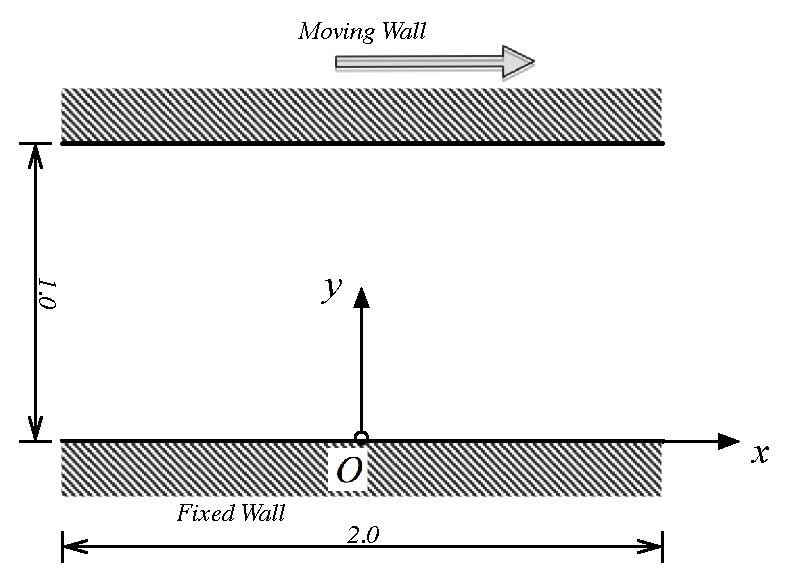
\includegraphics[width=8cm,clip]{PPLT2D.eps}
\end{center}
\caption{二次元平行平板間の計算空間.}
\label{fig:pplate2d}
\end{figure}
\end{comment}


%%
\subsection{IP\_Rectクラス}
IP\_Rectクラスは三次元の矩形の計算領域を表現するクラスです.
計算領域は,次のようにDomainファイルで指定します.
ここでは,各方向の格子幅を指定し,基点座標と計算領域の大きさを指定しています.


{\small
\begin{program}
DomainInfo {
  Global_origin   = (-0.5, -0.5, -0.5   )
  Global_region   = (1.0,  1.0,  1.0    )
  Global_pitch    = (1.5625e-02, 1.5625e-02, 1.5625e-02)
  ActiveSubDomain_File = ""
}
\end{program}
}


\begin{figure}[htdp]
\begin{center}
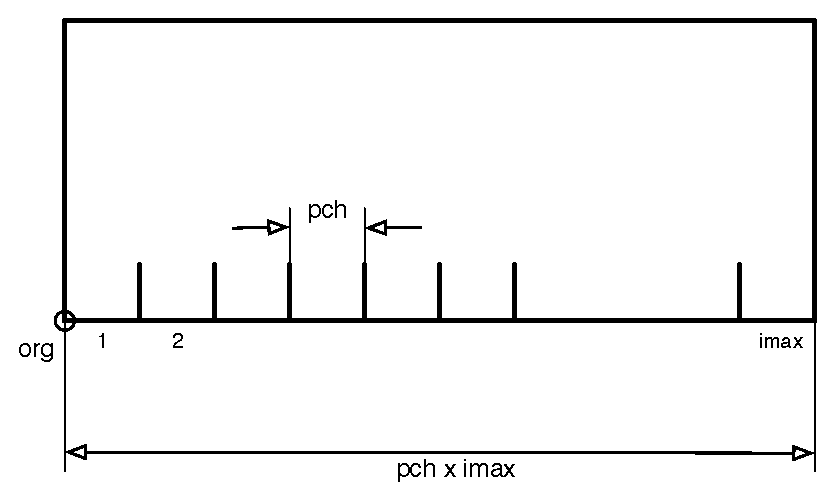
\includegraphics[width=9cm,clip]{rect.eps}
\caption{Rectangularクラスのパラメータ設定}
\label{fig:rect intrinsic class}
\end{center}
\end{figure}


\begin{table}[htdp]
\caption{Intrinsic\_Exampleタグで設定可能なパラメータ}
\begin{center}
\small
\begin{tabular}{lll}\toprule
指定パラメータ & 指定値 & 意味\\ \midrule
Check\_Even & Yes $|$ No & 分割数が偶数であるかどうかをチェックする\\
Fluid\_Medium & Medium\_Tableのラベル名 & 流体の媒質\\
Solid\_Medium & Medium\_Tableのラベル名 & 固体の媒質\\
\bottomrule
\end{tabular}
\end{center}
\label{tbl:rect parameter}
\end{table}

\textbf{表\ref{tbl:rect parameter}}のパラメータは,IP\_Rectクラスに固有の設定項目で,Parameter $>$ Intrinsic\_Exampleセクションで指定します.

{ \small
\begin{program}
  Intrinsic_Example {
    fluid_medium = "air"
    solid_medium = "fe"
    check_even = "yes"
  }
\end{program}
}

上記のパラメータ設定では,分割数の偶数チェックを行い,Medium\_TableにおいてAir,Feのラベル名で指定されている物性値を,それぞれ流体と固体として参照しています.



%
\begin{comment}
\subsection{IP\_Polygonクラス}
XMLファイルで,\lq\lq Steer > Solver\_Property > Shape\_Approximation\rq\rq でDistance\_Infoを指定すると,距離情報を用いたスキームで計算します.
この\hypertarget{tgt:polygon_class}{IP\_Polygonクラス}は,入力するポリゴンファイルと,DomainInfoで指定する計算領域情報のみで計算を行うモデルテンプレートです.ポリゴンファイル名は,\lq\lq Steer > Polygon\_File\rq\rq で指定します.
\end{comment}

%
\begin{comment}
\subsection{IP\_SHC1Dクラス}
\textbf{図\ref{fig:HC1D}}に示すような片持ちはりの熱伝導問題を一次元の定常熱伝導問題として解くためのクラスです.
この問題には厳密解があり,厳密解と計算結果を比較することにより予測精度の確認ができます.

\begin{figure}[htdp]
\begin{center}
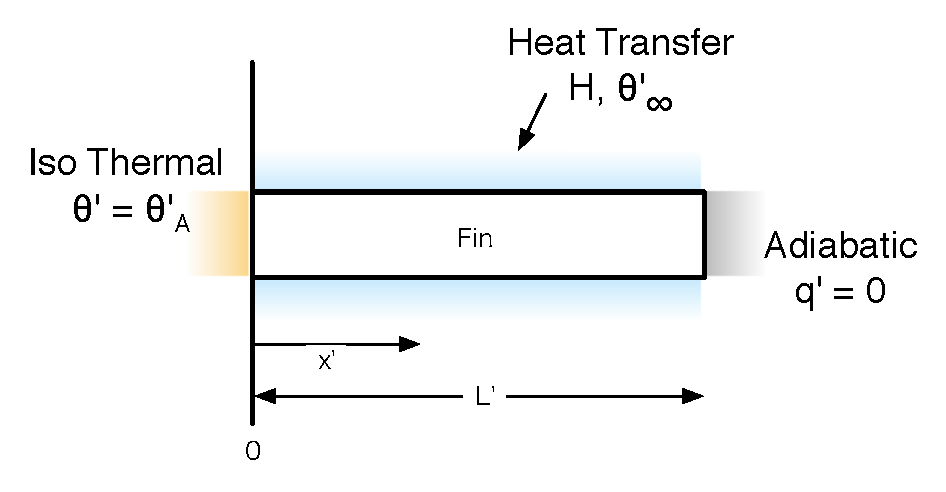
\includegraphics[width=9cm,clip]{1DHC.eps}
\end{center}
\caption{一次元定常熱伝導問題の模式図}
\label{fig:HC1D}
\end{figure}


計算領域は\textbf{図\ref{fig:HC model}}に示すようにx軸方向に放熱フィンをとり,y,z方向には5つだけセルを設けます.
領域の設定パラメータとして,x方向の分割数をimaxにより与えます.
放熱フィンを5分割したい場合には,imax=7を設定します.
その他の方向は$\mathrm{jmax=kmax=5}$で固定です.

例題と解析結果の詳細については,例題集をご覧ください.

\begin{figure}[htdp]
\begin{minipage}{0.47\hsize}
\begin{center}
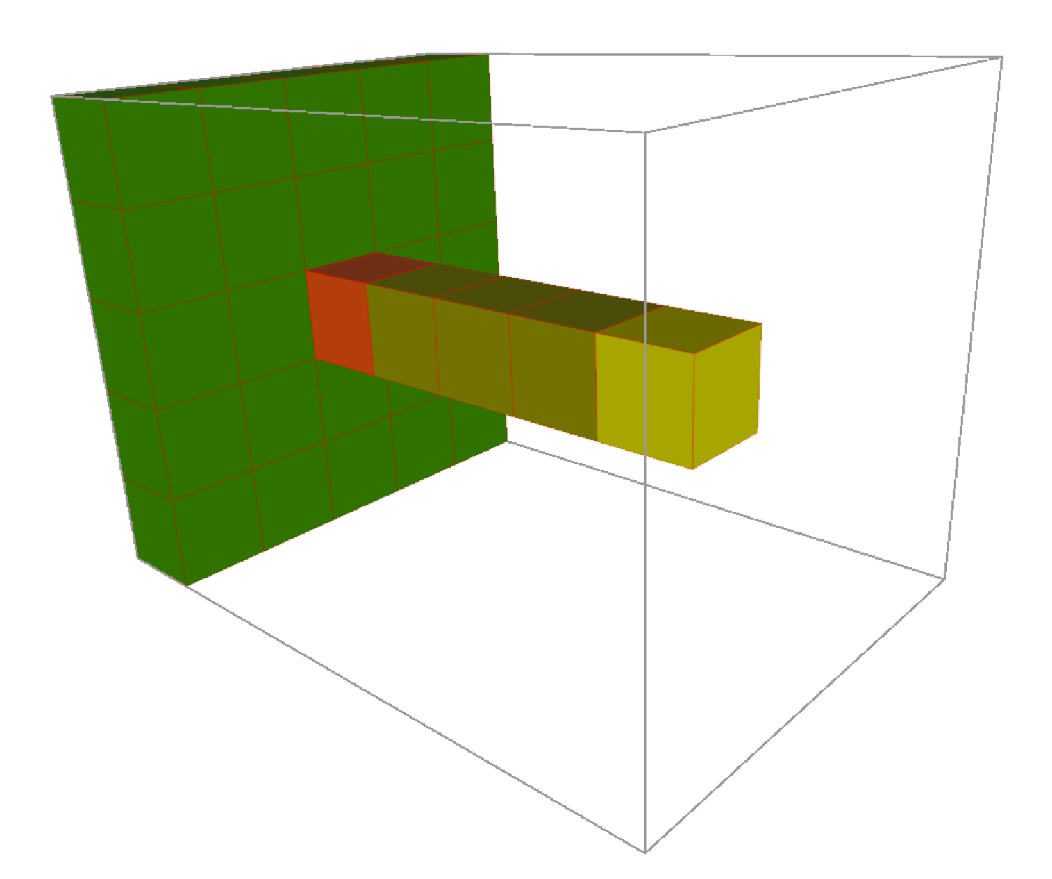
\includegraphics[height=5cm,clip]{model_iso.eps}
\end{center}
\end{minipage}
\begin{minipage}{0.47\hsize}
\begin{center}
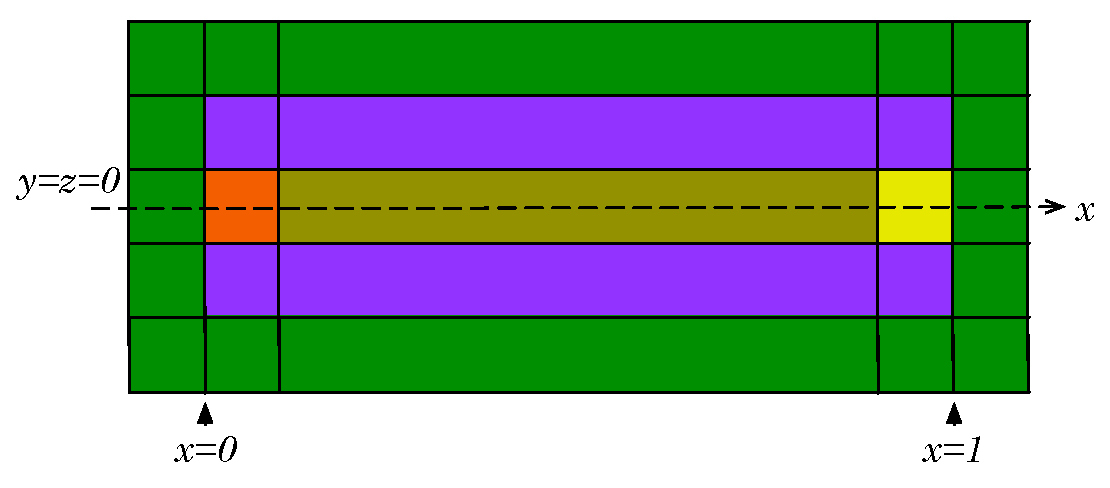
\includegraphics[height=3.5cm,clip]{dimension.eps}
\end{center}
\end{minipage}
\caption{一次元熱伝導問題を計算するための片持ち梁の三次元モデルとセルID (分割数が$7\times5\times5$の場合)}
\label{fig:HC model}
\end{figure}
\end{comment}

\pagebreak
% 
\section{例題}
ソースファイルのExampleディレクトリに含まれる\hypertarget{tgt:samples}{例題}について説明します.
提供される例題は,組み込みモデルや簡単なボクセルモデルを同梱した例題群で,
基本的な流れやソルバーの検証のために用意されています.


\begin{table}[htdp]
\caption{組み込み例題}
\begin{center}
\small
\begin{tabular}{lll} \toprule
Example & Class & Comment\\ \midrule
Cavity flow 3D (Cube) & IP\_Rect & 三次元立方体キャビティフロー\\
LDC112  & IP\_Rect & Guermondの実験に対応する辺長が1:1:2のキャビティフロー\\ 
%Duct 3D & IP\_Duct3D & ダクト流れ\\ 
PMT & IP\_PMT & 性能測定を行うための例題(三次元立方体キャビティフローの例題と同じ)\\
\bottomrule
\end{tabular}
\end{center}
\label{tbl:example at glance}
\end{table}


\begin{table}[htdp]
\caption{サンプル例題}
\begin{center}
\small
\begin{tabular}{lll} \toprule
Example & Comment\\ \midrule
%Dragon & Asian Dragon周りの流れ\\
%Heated Plate & 流体中の平板からの放熱\\
%SHC1D & 熱伝導計算の解析解との比較\\ \bottomrule
\end{tabular}
\end{center}
\label{tbl:exercise}
\end{table}





%%%
\chapter{制御と物理パラメータ}

\begin{abstract}
FFV-Cソルバーの入力パラメータは,記述性とマルチプラットホームでの稼働を考慮し,軽量の簡易パースライブラリ(TextParser)を利用しています.
構文は階層化され,テキストで容易に記述できます.
本章では,FFV-Cソルバーの制御と物理パラメータについて説明します.
\end{abstract}
%
\graphicspath{{./fig_Param/}}

%
\section{入力パラメータファイルの記述構文}
%
\subsection{パラメータ記述}
textparserライブラリが扱うパラメータデータベースは,下記のようにノードの階層構造にリーフ(ラベル/値のペア)を格納した構造になっています.パラメータ値のうち,文字列についてはダブルクォーテーションにより囲みます.
TextParserライブラリのExamplesディレクトリにパラメータの様々な記述例があるので,参考にしてください.

{
\small 
\begin{program}
  Time_Control {
    Acceleration_Type  = "Time"
    Acceleration       = 1.0
    Dt_Type            = "CFL_Reference_Velocity"
    Delta_T            = 0.2
    Period_Type        = "step"
    Calculation_Period = 20
  }
\end{program}
}


%
\subsection{パラメータファイルの種類と構造}
FFV-Cでは,\textbf{表\ref{tbl:input_files}}に示す2つの入力ファイルを使います.

\begin{table}[htdp]
\caption{パラメータファイル内のセクション}
\begin{center}
\small
\begin{tabular}{ll} \toprule
ファイル & 記述内容\\ \midrule
input.tp & 入力パラメータファイル\\
polygon.tp & 入力幾何形状ファイル\\ \bottomrule
\end{tabular}
\end{center}
\label{tbl:input_files}
\end{table}


パラメータファイルは,\textbf{表\ref{tbl:param_tag}}に示すセクションがあります.


\begin{table}[htdp]
\caption{パラメータファイル内のセクション}
\begin{center}
\small
\begin{tabular}{ll} \toprule
セクション & パラメータ\\ \midrule
DomainInfo & 計算領域情報\\
Steer & ソルバー制御\\
Parameter & 計算条件\\
BC\_Table & 境界条件\\
Medium\_Table & 媒質情報\\ \bottomrule
\end{tabular}
\end{center}
\label{tbl:param_tag}
\end{table}


起動時には,次のようにコマンドラインでタイプし実行します.
{
\small 
\begin{program}
$ ffvc input.tp
\end{program}
}




\pagebreak
%%
\section{入力パラメータファイル}


%
\subsection{DomainInfo}

計算対象となる領域の情報を与えます.

\begin{indentation}{3zw}{0zw}

{\small
\begin{program}
DomainInfo {
  Unit_of_length  = "M"
  Global_origin   = (-0.5, -0.5, -0.5   )
  Global_region   = (1.0,  1.0,  1.0    )
  Global_voxel    = (128   , 128   , 128   )
  
  //Global_pitch    = (1.5625e-02, 1.5625e-02, 1.5625e-02)
  //Global_division = (1    , 1    , 1    )

  ActiveSubDomain_File = "hoge"
}
\end{program}
}

計算領域情報については,\textbf{表\ref{tbl:region_info}}に示す計算領域に関するパラメータを指定します.

\begin{table}[htdp]
\caption{DomainInfoセクションにおける計算領域パラメータの指定}
\begin{center}
\small
\begin{tabular}{lll} \toprule
ラベル & 指定内容 & 補足\\ \midrule
Unit\_of\_Length & DomainInfoファイルに記述された長さの単位を指定する & (Non\_Dimensional $|$ M $|$ cm $|$ mm)\\
Global\_division & 並列計算時の各軸方向の分割数指定 & 任意\\ 
Global\_origin & 計算空間における座標値の最小値 & 必須\\
Global\_pitch & 各軸方向の分割幅 &Global\_voxelと排他,同時指定時に優先\\
Global\_region & 計算領域の大きさ & 必須\\ 
Global\_voxel & 計算空間の各軸方向の分割数 & Global\_pitchと排他\\
ActiveSubDomain\_File & サブドメインの活性・不活性を指定するファイル名 & ファイルがなければブランクを入力\\ \bottomrule
\end{tabular}
\end{center}
\label{tbl:region_info}
\end{table}

\end{indentation}



%
\pagebreak
\subsection{Steerセクション}

Steerセクションでは,実行制御パラメータ\index{じっこうせいぎょぱらめーた@実行制御パラメータ}を記述します.\\

%
\subsubsection{Algorithm}

時間積分と\hypertarget{tgt:algorithm}{解法アルゴリズム}の組み合わせを指定するパラメータです.

\begin{indentation}{3zw}{0zw}

{\small
\begin{program}
  Algorithm {
    Flow = "FS_C_EE_D_EE"
    Heat = "C_EE_D_EE"
  }
\end{program}
}

\textbf{表\ref{tbl:alg_flow}}に時間進行法と分離解法の種類の組み合わせを示します.Flowラベルでは流動の支配方程式の時間積分法と解法アルゴリズムの組み合わせを指定します.
%時間二次精度以上を選択した場合には,\verb|Convection_Term|\ref{sec:p_convection}では二次以上の空間スキームしか選択できません.\\

\begin{table}[htdp]
\caption{流動解析のアルゴリズム指定}
\begin{center}
\small
\begin{tabular}{ll} \toprule
ラベル & 時間積分法と解法の組み合わせ\\ \midrule
FS\_C\_EE\_D\_EE & Fractional Step法 + 時間一次精度Euler陽解法(対流項と拡散項)\\ \bottomrule
%FS\_C\_RK\_D\_CN & FS法 + 時間二次精度 Runge-Kutta陽解法(対流項)+ Crank-Nicholson陰解法(拡散項)\\
%FS\_C\_RK\_D\_ME & FS法 + 時間二次精度 Runge-Kutta陽解法(対流項)+ Modified-Euler陽解法(拡散項)\\
%FS\_C\_AB\_D\_AB & FS法 + 時間二次精度 Adams-Bashforth陽解法(対流項と拡散項)\\ \bottomrule
\end{tabular}
\end{center}
\label{tbl:alg_flow}
\end{table}

温度解析の場合には,Heatラベルで温度輸送方程式の時間進行法と解法アルゴリズムの組み合わせを\textbf{表\ref{tbl:alg_heat}}に示します.\\

\begin{table}[htdp]
\caption{温度解析のアルゴリズム指定}
\begin{center}
\small
\begin{tabular}{ll} \toprule
ラベル & 時間積分法と解法の組み合わせ\\ \midrule
C\_EE\_D\_EE & 時間一次精度 Euler陽解法(対流項と拡散項)\\
C\_EE\_D\_EI & 時間一次精度 Euler陽解法(対流項)+ Euler陰解法(拡散項)\\ \bottomrule
%C\_AB\_D\_AB & 時間二次精度 Adams-Bashforth陽解法(対流項と拡散項)\\ \bottomrule
\end{tabular}
\end{center}
\label{tbl:alg_heat}
\end{table}
\end{indentation}



%%%
\pagebreak
\subsubsection{Average\_Option}

\hypertarget{tgt:average_option}{時間平均操作}に関するパラメータを指定します.

\begin{indentation}{3zw}{0zw}

{\small
\begin{program}
  Average_option {
    Operation  = "Off"
    Start_Type = "Time"
    Start      = 500.0
  }
\end{program}
}

\textbf{表\ref{tbl:averaging}}に物理量の時間平均操作\index{じかんへいきんそうさ@時間平均操作}を指定するパラメータを示します.
FFV-Cソルバーは非定常解析を行いますので,流れの挙動が準定常状態になったところで時間平均操作を開始し,十分な長さで時間平均操作が行われた速度場や温度場を定常解\index{ていじょうかい@定常解}とみなします.
時間平均操作の開始時刻はStartで指定し,この開始時刻以降,毎ステップごとに時間平均操作を行います.
平均操作の開始時刻は,Start\_Typeで指定する方法に依存し,
Timeを指定した場合にはUnit\_of\_Input\_Parameterの次元に従います.
つまり,\hyperlink{tgt:unit}{DIMENSIONAL}の場合には有次元時刻で時間平均操作の開始時刻を指定することになります.

時間平均場の出力タイミングは,\hyperlink{tgt:fileio}{File\_IO}のAveraged\_Intervalで指定します.


\begin{table}[htdp]
\caption{Average\_Optionのパラメータ}
\begin{center}
\small
\begin{tabular}{ll} \toprule
ラベル & 指定パラメータ\\ \midrule
Operation & On $|$ Off\\
Start\_Type & 開始時刻の指定 (Step $|$ Time)\\
Start & 時間平均操作の開始時刻\\ \bottomrule
\end{tabular}
\end{center}
\label{tbl:averaging}
\end{table}

\end{indentation}



%%%
\pagebreak
\subsubsection{Check\_Parameter}

入力パラメータの初期化処理時の\hypertarget{tgt:check_parameter}{整合性のチェック}を行い,初期設定後にソルバーを停止します.

\begin{indentation}{3zw}{0zw}

{\small
\begin{program}
  Check_Parameter = "Off"
\end{program}
}

Check\_Parameter=\lq\lq On\rq\rq でチェックが有効な場合,FFV-Cを起動してパラメータを読み込み,前処理が終了した段階で強制終了します.
このとき,初期設定パラメータの内容がconditions.txtに書き出されているので,パラメータのチェックができます.
また,初期条件を与えたフィールドファイルが出力されるので,初期条件のチェックが可能です.

\end{indentation}



%%%
\pagebreak
\subsubsection{Convection\_Term}

\hypertarget{tgt:convection_term}{対流項のスキーム}に関するパラメータを指定します.

\begin{indentation}{3zw}{0zw}

{\small
\begin{program}
  Convection_Term {
    Scheme  = "O3_MUSCL"
    Limiter = "minmod"
  }
\end{program}
}

SchemeとLimiterのパラメータを\textbf{表\ref{tbl:scheme limiter}}に示します.Limiterは制限関数\index{せいげんかんすう@制限関数}の種類を示し,Schemeが\verb|O3_MUSCL|の場合のみ有効となります.
非圧縮流れのように物理量の変化が連続的な場合には不要の場合もあります.
ファイル出力時のオプションでガイドセル出力\hyperlink{tgt:fileio}{Guide\_Out}=\lq\lq with\rq\rq を指定している場合には,対流項スキームによってステンシル\index{ステンシル}が変化するので,ガイドセル\index{ガイドセル}の値も異なります.

\begin{table}[htdp]
\small
\caption{SchemeとLimiterのパラメータ}
\begin{minipage}{.6\textwidth}
\begin{center}
\begin{tabular}{llc} \toprule
ラベル& 指定スキーム & 出力ガイドセルサイズ\\ \midrule
O1\_Upwind & 一次精度風上スキーム & 1\\
O2\_Central & 二次精度中心スキーム & 1\\
O3\_MUSCL & 三次精度MUSCLスキーム & 2\\ \bottomrule
\end{tabular}
\end{center}
\end{minipage} \hfill
\begin{minipage}{.38\textwidth}
\begin{center}
\begin{tabular}{ll} \toprule
ラベル & 制限関数\\ \midrule
Minmod & minmod型\\
No\_Limiter & | \\ \bottomrule
\end{tabular}
\end{center}
\end{minipage}
\label{tbl:scheme limiter}
\end{table}

\end{indentation}



%%%
\pagebreak
\subsubsection{Derived\_Variable}

\hypertarget{tgt:derived_variable}{派生変数}(基本変数から計算される変数)の生成を指定します.

\begin{indentation}{3zw}{0zw}

{\small
\begin{program}
  Derived_Variable {
    Total_Pressure       = "Off"
    Helicity             = "Off"
    Vorticity            = "Off"
    2nd_Invariant_of_VGT = "Off"
  }
\end{program}
}

\textbf{表\ref{tbl:derived vars}}に示す各変数は,on/offのスイッチ指定により有効・無効になり,\hyperlink{tgt:fileio}{File\_IO}セクションのInstant\_Intervalで指定するタイミングでファイルに出力されます.

\begin{table}[htdp]
\caption{派生変数の指定}
\begin{center}
\small
\begin{tabular}{ll}\toprule
ラベル & 生成する派生変数\\ \midrule
Total\_Pressure & 全圧\\
Vorticity & 渦度ベクトル\\
Helicity & ヘリシティ\\
2nd\_Invariant\_of\_VGT & 速度勾配テンソルの第二不変量\\ \bottomrule
\end{tabular}
\end{center}
\label{tbl:derived vars}
\end{table}

%
\paragraph{全圧(総圧)}
全圧の計算を指定した場合には,\verb|tp*.sph|のファイル名でファイルが出力されます\footnote{ワイルドカード*には,ステップ数や並列計算時にはランク番号が入ります}.


全圧は次式で定義され,単位体積あたりのエネルギーを表します.

\begin{equation}
\frac{1}{2} {u^{\prime}}^{2} + \frac{P^{\prime}}{\rho^{\prime}} \qquad [Pa] \sim [J/m^3]
\label{eq:total pressure}
\end{equation}

非圧縮の場合には,

\begin{equation}
{P_{T}}^{\prime} \,=\, \frac{1}{2} \rho^{\prime} {u^{\prime}}^{2} + P^{\prime} \qquad [J/m^3]
\label{eq:total pressure icmp}
\end{equation}

\textbf{式(\ref{eq:total pressure icmp})}は無次元化すると,以下のようになります.

\begin{equation}
P_{T} \,=\, \frac{{P_{T}}^{\prime}}{\rho_{\mathit{0}}^{\prime} {u_{\mathit{0}}^{\prime}}^{2}}
\label{eq:total pressure icmp ND}
\end{equation}

%
\paragraph{渦度ベクトル}
渦度の計算を指定した場合には,\verb|vrt*.sph|のファイル名でファイルが出力されます.

%
\paragraph{ヘリシティ}
ヘリシティの計算を指定した場合には,\verb|hty*.sph|のファイル名でファイルが出力されます.
ヘリシティは速度ベクトル$\overrightarrow{u}$と渦度ベクトル$\overrightarrow{\omega}$の内積として定義される量で次式により表せます.

\begin{equation}
H \,=\, \overrightarrow{u} \cdot \overrightarrow{\omega}
\label{eq:helicity}
\end{equation}


%
\paragraph{速度勾配テンソルの第二不変量}
渦構造を可視化するのに利用され,
符号により単純剪断乱流の中の層状渦と管状渦を区別することができます\cite{tanaka:93:PF}.
\verb|i2vgt*.sph|のファイル名でファイルが出力されます.

\end{indentation}



%%%
\pagebreak
\subsubsection{Example}

\hypertarget{tgt:example}{解くべき問題}を指定します.

\begin{indentation}{3zw}{0zw}

{\small
\begin{program}
  Example = "Performance_Test"
\end{program}
}

\textbf{表\ref{tbl:intrinsic_example}}にFFV-Cソルバーが提供する組み込み例題\index{くみこみれいだい@組み込み例題}の一覧を示します.
組み込み例題で例題固有のパラメータ設定については,Parameter$\to$\hyperlink{tgt:intrinsic_example}{Intrinsic\_Example}をご覧ください.

また,具体的な例題の事例については,例題集をご覧ください.

\begin{table}[htdp]
\caption{Exampleのパラメータ指定}
\begin{center}
\small
\begin{tabular}{ll} \toprule
ラベル & 例題\\ \midrule
Back\_Step & バックステップ形状\\
Cylinder & 円柱・角柱\\
Duct & 直方体と円形断面のダクト\\
Parallel\_Plate\_2D & 二次元の並行平板\\
Performance\_Test & 性能評価\\
Rectangular & 矩形計算領域の問題\\
SHC1D & 固体熱伝導\\ 
Sphere & 球\\ 
Users & ユーザ例題\\ \bottomrule
\end{tabular}
\end{center}
\label{tbl:intrinsic_example}
\end{table}

\end{indentation}


%%%
\pagebreak
\subsubsection{File\_IO}

\hypertarget{tgt:fileio}{ファイル入出力モード}を指定します.このセクションでは,入出力ファイルの単位,ガイドセルのモード,並列入出力モード,デバッグ時のファイルなどを指定します.

\begin{indentation}{3zw}{0zw}

{\small
\begin{program}
  File_IO {
    Unit_of_File           = "Non_Dimensional"
    Guide_Out              = "Without"
    Debug_Divergence       = "Off"
    Instant_Interval_Type  = "step"
    Instant_Interval       = 1000
    Averaged_Interval_Type = "Time"
    Averaged_Interval      = 1000
    Voxel_Output           = "off"
    
    Output_Mode {
      Mode                 = "specified"
      Directory_Path       = "hoge"
    }
    
    Plot3d {
      Option               = "on"
      Interval_Type        = "step"
      Interval             = 10
    }
  }
\end{program}
}

\textbf{表\ref{tbl:file_IO_parameter}}に指定するパラメータの内容を示します.
Unit\_of\_Fileでは入出力する結果ファイルの単位を指定し,有次元か無次元を指定できます.

Guide\_Outラベルで\lq\lq with\rq\rq を指定した場合の出力ガイドセルのサイズは\hyperlink{tgt:convection_term}{Convection\_Term}の項を参照してください.


\begin{table}[htdp]
\caption{ファイル入出力のパラメータ指定}
\begin{center}
\small
\begin{tabular}{llll} \toprule
ラベル & 指定項目 & ラベル & 指定内容 \\ \midrule
Unit\_of\_File & 入出力ファイルの単位 & Dimensional & 有次元\\
& & Non\_Dimensional & 無次元\\ \hline
Guide\_Out & ガイドセル出力モード & with & ガイドセルを一緒に出力\\
& & without & 内部領域のみ出力\\ \hline
Debug\_divergence & デバッグ時のファイル出力 & On $|$ Off & $\nabla \cdot \bm{u}$の出力(無次元値)\\ \hline
Instant\_Interval\_Type & 瞬時値の出力指定形式 & Step & ステップ数指定\\
& & Time & 時間間隔の指定\\
Instant\_Interval & 出力間隔 & | & ステップ数$|$時間間隔\\ \hline
Averaged\_Interval\_Type & 平均値の出力指定形式 & Step & ステップ数指定\\
& & Time & 時間間隔の指定\\
Averaged\_Interval & 出力間隔 & | & ステップ数$|$時間間隔\\ \hline
Voxel\_Output & ボクセルファイルの出力指定 & | & off\\
 & & bx & ビットボクセル\\
 & & svx & svx フォーマット\\ \hline
Output\_Mode & & & \\
Mode & 出力ディレクトリモード & current & ソルバー起動ディレクトリに出力\\
 & & specified & 指定ディレクトリに出力\\
 & & time\_slice & 出力時刻毎にディレクトリを作成して出力\\
Directory\_Path & 出力ディレクトリを指定 & & ディレクトリパスを記述\\ \hline
PLOT3D & & & \\
Option & PLOT3D形式での出力 & On $|$ Off & \\
Interval\_Type & 出力指定形式 & Step & ステップ数指定\\
 & & Time & 時間間隔の指定\\
Interval & 出力間隔 & | & ステップ数$|$時間間隔\\
\bottomrule
\end{tabular}
\end{center}
\label{tbl:file_IO_parameter}
\end{table}


Debug\_Divergenceは,デバッグのため$\nabla \cdot \bm{u}$の値を無次元で出力します.

Intervalのラベルにより,ファイル出力間隔を指定します.
対象となる出力ファイルに対して,時刻またはステップ数によりファイル出力間隔を指定できます.
Instant\_Interval\_TypeあるいはAveraged\_Interval\_Typeが\lq\lq time\rq\rq の場合,時刻の単位は\hyperlink{tgt:unit}{Unit\_of\_Input\_Parameter}で指定したモードに従います.

Voxel\_Outputは,ボクセルファイルを確認のため出力する場合に利用し,ファイル形式を指定します.

Output\_Modeは,ファイルの出力方法を指定します.FFV-Cソルバーは大規模並列実行を想定しています.
つまり,多数のプロセスが各々の担当領域の結果をファイルに出力する場合,1つのディレクトリのファイル数が多くなり,ハンドリングが困難になります.これを回避するため,time\_sliceモードを用意しています.
このtime\_sliceモードは,出力のタイミング毎にディレクトリを自動的に作成し,そのディレクトリ内に結果ファイルを出力します.例えば,2,000プロセスで計算し,速度と圧力,および全圧の結果を出力することを指定すると,1時刻につき6,000ファイルが生成されますが,それ以上にはなりません.

PLOT3Dの出力については,PLOT3D\_Optionsセクションで詳細な指定が行えます.

\end{indentation}



%%%
\pagebreak
\subsubsection{Polygon\_File}
計算に用いる\hypertarget{tgt:poly_file_name}{ポリゴンファイル名}を指定します.

\begin{indentation}{3zw}{0zw}

幾何形状ファイルを指定で計算をする場合には,Exampleで\hyperlink{tgt:example}{users}を指定します.

{\small
\begin{program}
  Geometry_Model {
    Polylib_File          = "foo.tp"
    Fluid_Medium_for_Fill = "air"
    Solid_Medium_for_Fill = "fe"
    Hint_of_Filling_Fluid = "z_plus"
  }
\end{program}
}


\begin{table}[htdp]
\caption{幾何形状のパラメータ指定}
\begin{center}
\small
\begin{tabular}{llll} \toprule
ラベル & 指定項目 & ラベル & 指定内容 \\ \midrule
Polylib\_File & Polylibへの入力ファイル & & テキストパーサー形式\\
Fluid\_Medium\_for\_Fill & フィルを実行する場合の流体媒質名 & & \\
Solid\_Medium\_for\_Fill & フィルを実行する場合の固体媒質名 & & \\
Hint\_of\_Filling\_Fluid & フィルを実行する場合の基点のヒント & X\_Minus & X-方向からフィル\\
& & X\_Plus  & X+方向からフィル\\
& & Y\_Minus & Y-方向からフィル\\
& & Y\_Plus  & Y+方向からフィル\\
& & Z\_Minus & Z-方向からフィル\\
& & Z\_Plus  & Z+方向からフィル\\
\bottomrule
\end{tabular}
\end{center}
\label{tbl:file_geometry}
\end{table}

Fluid\_Medium\_for\_FillとSolid\_Medium\_for\_Fillは,Medium\_Tableで指定されている媒質ラベルを指定します.

\end{indentation}



%%%
\pagebreak
\subsubsection{Iteration}

圧力のポアソン方程式や陰解法のように,得られる線形システムの係数行列が大型疎行列となる場合には反復解法\index{はんぷくかいほう@反復解法}を用います.
ここでは流れと温度解析について,\hypertarget{tgt:iteration}{反復法のパラメータを指定}します.

\begin{indentation}{3zw}{0zw}

{\small
\begin{program}
  Iteration {
    Flow {
      Poisson {
        Iteration     = 50
        Epsilon       = 1.0e-4
        Omega         = 1.1
        Norm          = "r_r0"
        Linear_Solver = "sor2sma"
        Comm_mode     = "async"
      }
      VP {
        Iteration     = 100
        Epsilon       = 1.0e-4
        Norm          = "v_div_max"
      }
    }
    Heat {
      Euler_Implicit {
        Iteration     = 30
        Epsilon       = 1.0e-2
        Omega         = 1.1
        Norm          = "T_Res_L2_Absolute"
        Linear_Solver = "SOR"
        Comm_mode     = "sync"
      }     
    }     
  }
\end{program}
}

FFV-Cの反復過程は,フラクショナルステップ法を基本としていますが,ダルシー則のような速度の関数で圧力勾配が決まるような境界条件を陰的に扱えるように工夫されています.
このため,HSMACのように圧力のアップデートと同時に速度のアップデートも毎回行い,$\bm{u}^{n+1}$の値を毎回計算し,$\nabla \cdot \bm{u}^{n+1}$を評価し,速度の発散が指定値以下になったら収束したと判断しています.
つまり,圧力Poissonの収束と速度の発散値の収束の2つの閾値で収束判定を行っています.

反復法を用いる場合は,\hyperlink{tgt:algorithm}{Algorithm}セクションで反復法を含む解法を指定します.

%第2レベルで指定するラベルは指定するアルゴリズムに応じて異なります.
%\textbf{表\ref{tbl:itr_flow_algo}}に指定アルゴリズムと指定ラベルの関係を示します.
%2nd\_Poissonは二次精度Runge-Kutta法の場合の2nd stepの圧力反復の収束条件を意味します.

\textbf{表\ref{tbl:flow_itr}}には,流動解析の反復解法の指定パラメータを示します.
圧力のPoisson反復式に指定可能な収束判定ノルムの種類を\textbf{表\ref{tbl:norm-type Poisson}}に示します.
また,圧力速度の反復過程の収束条件は\textbf{表\ref{tbl:norm-type VP}}で指定します.

\textbf{表\ref{tbl:LS}}に選択できる反復解法を示します.
表中の△は,並列処理時のデータ依存性(再帰干渉)のために,逐次と並列時で異なる収束特性を示すことを意味します.
%SOR2CMAは反復過程でメモリアクセスが連続になるように並べ替えを行うためにオーバーヘッドが生じるので,反復回数が少ない場合には計算速度向上の効果はない.\\

%\begin{table}[htdp]
%\caption{流動解析のアルゴリズムと指定ラベル}
%\begin{center}
%\small
%\begin{tabular}{ll} \toprule
%Algorithm & 必要なラベル\\ \midrule
%FS\_C\_EE\_D\_EE & Poisson\\ \bottomrule
%FS\_C\_AB\_D\_AB & Poisson\\ \bottomrule
%FS\_C\_RK\_D\_ME & 1st\_Iteration, 2nd\_Iteration\\
%FS\_C\_RK\_D\_CN & 1st\_Iteration, 2nd\_Iteration\\ \bottomrule
%\end{tabular}
%\end{center}
%\label{tbl:itr_flow_algo}
%\end{table}

\begin{table}[htdp]
\caption{反復条件の指定}
\begin{center}
\small
\begin{tabular}{ll} \toprule
ラベル & 指定内容\\ \midrule
Iteration & 最大反復回数\\
Epsilon & 収束閾値\\
Omega & 加速(緩和)係数\\
Norm & 収束ノルムの種類\\ 
Linear\_Solver & 反復法の指定\\ \hline
Comm\_Mode & 袖通信のモード\\
 & "Sync" 同期通信モード\\
 & "Async" 非同期通信モード\\ \bottomrule
\end{tabular}
\end{center}
\label{tbl:flow_itr}
\end{table}


\begin{table}[htdp]
\caption{流動計算における圧力Poisson反復のノルムの指定}
\begin{center}
\small
\begin{tabular}{lll} \toprule
ラベル & 収束判定基準 & 評価式\\ \midrule
dx\_b & 反復相対残差の$L_2$ノルムを右辺ベクトルの$L_2$ノルムで除したもの & $\|x^{m+1}-x^m \|_2 \bigg / \|b\|_2$\\
\vspace{2mm}
r\_b & 残差の$L_2$ノルムを右辺ベクトルの$L_2$ノルムで除したもの & $\| r \|_2 \bigg / \|b\|_2$\\
\vspace{2mm}
r\_r0 & 残差の$L_2$ノルムを初期残差ベクトルの$L_2$ノルムで除したもの & $\|r\|_2 \bigg / \|r_0\|_2$\\ 
\bottomrule
\end{tabular}
\end{center}
\label{tbl:norm-type Poisson}
\end{table}


\begin{table}[htdp]
\caption{流動計算における圧力速度の同時反復のノルムの指定}
\begin{center}
\small
\begin{tabular}{lll} \toprule
ラベル & 収束判定基準 & 評価式\\ \midrule 
v\_div\_max & 発散の最大値 & $max\left|div\,\bm{u}\right|$\\
\vspace{2mm}
v\_div\_dbg & 発散の最大値の値とセル位置を出力する\footnotemark[1] & $max\left|div\,\bm{u}\right|$\\
\bottomrule
\end{tabular}
\end{center}
\label{tbl:norm-type VP}
\end{table}
\footnotetext[1]{サーチを行うので,実行速度は遅くなる(デバッグ利用).}


\begin{table}[htdp]
\caption{Linear\_Solverの選択}
\begin{center}
\small
\begin{tabular}{llc} \toprule
ラベル & 反復解法 & 並列計算への適用\\ \midrule
%Jacobi & 緩和Point Jacobi法 & ○\\
SOR & Point SOR法 & △\\
%SOR2CMA & 連続メモリアクセス型の2色SOR法\\
SOR2SMA & ストライドメモリアクセス型の2色SOR法 & ○\\ 
GMRES & GMRES(m) リスタート周期 m & ○\\ 
\bottomrule
\end{tabular}
\end{center}
\label{tbl:LS}
\end{table}




温度計算で反復法を用いる場合は,\hyperlink{tgt:algorithm}{Algorithm}セクションで反復法を含む解法を指定します.

Flow, Heatのラベルは,それぞれ,流れ計算と熱計算のパラメータであることを示します.
\textbf{表\ref{tbl:itr_temp_algo}}に,指定アルゴリズムと指定ラベルの関係を示します.

温度解析の反復解法のパラメータと収束ノルムのタイプは,それぞれ\textbf{表\ref{tbl:flow_itr}},\textbf{表\ref{tbl:norm-type Poisson}}と同様です.

\begin{table}[htdp]
\caption{温度解析のアルゴリズムと指定ラベル}
\begin{center}
\small
\begin{tabular}{ll} \toprule
Algorithm &  必要なラベル\\ \midrule
C\_EE\_D\_EE & | \\
%C\_AB\_D\_AB & なし\\
C\_EE\_D\_EI & Euler\_Implicit\\ \bottomrule
\end{tabular}
\end{center}
\label{tbl:itr_temp_algo}
\end{table}

\end{indentation}



%%%
\pagebreak
\subsubsection{LES\_Option}

\hypertarget{tgt:les_option}{LES}(Large-Eddy Simulation)のオプションパラメータを指定します\footnote{\today 現時点で機能未実装.}.

\begin{indentation}{3zw}{0zw}

{\small
\begin{program}
  LES_Option {
    LES_Calculation = "Off"
  }
\end{program}
}

指定できるLESのモデルを\textbf{表\ref{tbl:LES_model}}に示します.

\begin{table}[htdp]
\caption{LESのモデル指定}
\begin{center}
\small
\begin{tabular}{ll} \toprule
ラベル & モデル\\ \midrule
Smagorinsky & 標準スマゴリンスキーモデル\\ \bottomrule
%Low\_Reynolds & 低レイノルズ数型モデル\\
%Dynamic & ダイナミックモデル\\ \bottomrule
\end{tabular}
\end{center}
\label{tbl:LES_model}
\end{table}

\end{indentation}



%%%
\pagebreak
\subsubsection{Log}

\hypertarget{tgt:log}{各種履歴}ファイル\index{ふぁいる@ファイル!りれき@履歴---}出力の制御パラメータを指定します.

\begin{indentation}{3zw}{0zw}

{\small
\begin{program}
  Log {
    Unit_of_Log           = "Non_Dimensional"
    Log_Base              = "On"
    Log_Iteration         = "Off"
    Log_Profiling         = "on"
    Log_Wall_Info         = "Off"
    Console_Interval_Type = "Step"
    Console_Interval      = 1
    History_Interval_Type = "Step"
    History_Interval      = 1
  }
\end{program}
}

Log\_Baseラベルでは,基本履歴ファイルのon/offを制御します.つまり,標準モニタ出力やコンポーネント情報,領域の流量収支履歴の出力を制御します.

Log\_Iterationラベルは,各タイムステップの反復数,残差の最大値とそのインデクス値などの圧力の反復過程の履歴を出力します.
このラベルを \lq\lq on\rq\rq に指定すると,残差は強制的に\hyperlink{tgt:iteration}{V\_Div\_Max}(発散の最大値)となり,\hyperlink{tgt:iteration}{Interation}ラベルでのノルムの指定は無効になります.反復履歴は他の種類のノルムには対応していません.

Log\_Profilingラベルは,実行時に性能測定のための計時を行い,結果をレポートとして出力することを指定します.
Detailオプションにより,詳細なレポートを出力します.
出力項目の詳細は,\hyperlink{tgt:profile}{性能情報}をご覧ください.

Log\_Wall\_Infoは,\hyperlink{tgt:treatment_of_wall}{壁法則}を用いた場合の種々の情報を出力しますが,試験的なものです.

Intervalのラベルにより,ファイル出力間隔を指定します.
対象となる出力ファイルに対して,時刻またはステップ数によりファイル出力間隔を指定できます.
Console\_Interval\_TypeあるいはHistory\_Interval\_Typeがvalue=\lq\lq time\rq\rq の場合,時刻の単位は\hyperlink{tgt:unit}{Unit\_of\_Input\_Parameter}で指定したモードに従います.

Unit\_of\_Logではログ出力の有次元・無次元を指定します.

\begin{table}[htdp]
\caption{履歴ファイルの出力指定}
\begin{center}
\small
\begin{tabular}{lll} \toprule
ラベル & 指定内容 & ラベル$|$指定内容\\ \midrule
Log\_Base & 標準履歴ファイル & ON $|$ OFF\\
Log\_Iteration & 反復解法の反復履歴 & ON $|$ OFF\\
Log\_Profiling & 実行性能レポートの作成・出力 & ON $|$ OFF\\
Log\_Wall\_Info & 壁面情報履歴 & ON $|$ OFF\\ \hline
Console\_Interval\_Type & 標準出力の出力指定形式 & Step (ステップ数指定)\\
& & Time (時刻指定)\\
Console\_Interval & 出力間隔 & ステップ数 $|$ 時刻\\ \hline
History\_Interval\_Type & 履歴ファイルの出力指定形式 & Step (ステップ数指定)\\
& & Time (時刻指定)\\
History\_Interval & 出力間隔 & ステップ数 $|$ 時刻\\ \hline
Unit\_of\_Log & ログファイル中の記述単位 & Dimensional $|$ Non\_Dimensional\\\bottomrule
\end{tabular}
\end{center}
\label{tbl:log_output}
\end{table}

\end{indentation}





%%%
\pagebreak
\subsubsection{Monitor\_List}

ユーザが指定した物理量を指定した位置で\hypertarget{tgt:monitor_list}{サンプリング}し,ファイルに出力する機能です.
サンプリングして出力する機能は2通りの方法で実装されています.
ここでは,指定した座標点で計算結果をサンプリングし,ファイルに出力する方法について説明します.
詳細は,第\ref{chpt:monitor}章をご覧ください.
もう一つの指定方法は,モデルに与えられたラベルを用いて指定する方法で,これについては\hyperlink{tgt:localboundary}{境界条件}セクションをご覧ください.

\begin{indentation}{3zw}{0zw}

{\small
\begin{program}
  Monitor_List {
    Log                    = "Off"
    Output_File            = "sample.log"
    Output_Mode            = "Gather"
    Unit                   = "Non_Dimensional"
    Sampling_Interval_Type = "step"
    Sampling_Interval      = 100
    Cell_Monitor           = "off"

    list[@] {
      type            = "Line"
      label           = "line1"
      value           = "x"
      Variable        = "Velocity"
      Sampling_Method = "Interpolation"
      Sampling_Mode   = "Fluid"
      Division        = 64
      From            = (-0.5, 0.0, 0.0)
      To              = (0.5, 0.0, 0.0)
    }

    list[@] {
      type            = "Line"
      label           = "line2"
      Variable        = "Velocity"
      Sampling_Method = "Interpolation"
      Sampling_Mode   = "Fluid"
      Division        = 64
      From            = (0.0, 0.0, -0.5)
      To              = (0.0, 0.0, 0.5)
    }
  }
\end{program}
}

指定パラメータを\textbf{表\ref{tbl:monitor list}}に示します.
Monitor\_Listには,点群(point\_set)と線分(line)の2種類の指定方法があります.
それぞれをグループと呼び,point\_setの構成点をsetと定義します.

\begin{table}[htdp]
\caption{モニタリストでの指定パラメータ}
\begin{center}
\small
\begin{tabular}{lll} \toprule
ラベル & 指定ラベル & 指定内容\\ \midrule
Log & On $|$ Off & ログ出力指定\\
Output\_Mode & Gather & マスタープロセスに集約して出力\\
& Distribute & 各プロセス毎に出力\\
Unit & 入力パラメータと出力単位の指定 & Dimensional $|$ Non\_Dimensional\\
Sampling\_Interval\_Type & Step $|$ Time & 出力形式の指定\\
Sampling\_Interval & | & 指定間隔\\ 
Cell\_Monitor & On $|$ Off & モニタ出力指定\\ \hline
Point\_Set & & 点群によりモニタ点を指定する\\
Set & & 点の座標を指定する\\
x,y,z & & 座標\\ \hline
Line & & 線分によりモニタ点を指定する\\
From & & 開始点を指定する\\
To & & 終了点を指定する\\
x,y,z & & 座標\\ \hline
Variable & Velocity & 速度を指定\\
 & Pressure & 圧力\\
 & Temperature & 温度\\
 & Total\_Pressure & 全圧\\
 & Vorticity & 渦度\\ \hline
%Velocity\_average & 速度の平均値\\
%Pressure\_average & 圧力の平均値\\
%Temperature\_average & 温度の平均値\\
%Total\_Pressure\_average & 全圧の平均値\\
Sampling\_Method & Nearest & モニタ指定点を含むセルの値\\
 & Interpolation & 三重線形内挿補間\\
 & Smoothing & 局所平均による平滑化\\ \hline
Sampling\_Mode & All & 全セルを対象とする\\
 & Fluid & 流体セルのみを対象とする\\
 & Solid & 固体セルのみを対象とする\\ \bottomrule
\end{tabular}
\end{center}
\label{tbl:monitor list}
\end{table}

\begin{itemize}
\item モニタ出力機能は,LogラベルでON/OFFを指定します.
\item 出力ファイル名は,Output\_Fileラベルで指定します.
\item 出力モードはOutput\_Modeラベルで指定します.
これは並列計算時のファイル出力方式で,マスターノードに集約してファイル出力する場合にはGatherを指定し,分散ノード毎にファイル出力する場合にはDistributeを指定します.
\item Variableラベルでは,サンプリングする物理量を指定します.
物理量はpoint\_setの例のように複数指定可能です.
\item Sampling\_Methodラベルで指定されるパラメータは,サンプリング方法を指定します.
\item Sampling\_Modeで指定されるパラメータは,サンプリングモードを指定します.
\item ファイル出力間隔は,Sampling\_Intervalで指定し,その指定単位をSampling\_Interval\_Typeで指定します.
\item Unitラベルでは,Monitor\_Listセクションで指定するパラメータの単位と出力するログの単位を指定します.指定パラメータと出力ログの単位は同じになります.
\end{itemize}

\end{indentation}


%%%
\pagebreak
\subsubsection{PLOT3D\_Options}

PLOT3Dフォーマットで,結果を出力する場合のオプションを記述します.

\begin{indentation}{3zw}{0zw}
\small

\begin{program}
  PLOT3D_Options {
    filename         = "hoge"
    grid_kind        = "single_grid"
    grid_mobility    = "immovable"
    state_of_time    = "unsteady"
    set_iblank_flag  = "on"
    Dimension        = "3D"
    Format_type      = "unformatted"
    Output_xyz       = "on"
    Output_q         = "on"
    Output_function  = "on"
    Output_func_name = "on"
    Output_fvbnd     = "on"
    Divide_func      = "off"
    real_type        = "float"
  }
\end{program}

\end{indentation}



%%%
\pagebreak
\subsubsection{Reference\_Frame}

\hypertarget{tgt:reference_frame}{観測}の座標系\index{ざひょうけい@座標系}を指定します.

\begin{indentation}{3zw}{0zw}
\small

\begin{program}
  Reference_Frame {
    Reference_Frame_Type = "Stationary"
  }

\end{program}

\normalsize
FFV-Cソルバーでは,\textbf{表\ref{tbl:ref_frame}}に示す選択肢があります.
移動座標系\index{ざひょうけい@座標系!いどう@移動---}を指定する場合には,格子の移動速度の各方向成分(有次元では$[m/s]$)を入力します.
座標系は右手系をとり,各軸x, y, z方向の速度成分をそれぞれu, v, wとします.
静止座標系\index{ざひょうけい@座標系!せいし@静止---}と移動座標系とでは,同じ問題を解く場合でも与える境界条件が異なるので注意します.

\begin{table}[htdp]
\caption{Reference\_Frameの指定}
\begin{center}
\small
\begin{tabular}{lll} \toprule
ラベル & 指定パラメータ & 参照座標系\\ \midrule
Stationary & | & 静止座標系\\
Translational & $u,\,v,\,w$ & 並進運動する移動座標系\\ \bottomrule
%Rotational & $u,\,v,\,w$ & 回転運動する座標系\\ \bottomrule
\end{tabular}
\end{center}
\label{tbl:ref_frame}
\end{table}

\end{indentation}



%%%
\pagebreak
\subsubsection{Start\_Condition}

計算の\hypertarget{tgt:start_condition}{スタート条件}を指定します.

\begin{indentation}{3zw}{0zw}

{\small
\begin{program}
  Start_Condition {
    start_type         = "initial"
    Restart_step       = 200

    Restart_from_Different_Nproc {
      Staging = "on"
      Prefix_of_dir = "hoge_restart_"
      Prefix_of_Pressure = "prs_dr_"
      Prefix_of_Velocity = "vel_dr_"
    }

    DFI_file {
      pressure  = "prs_dr_.dfi"
      velocity  = "vel_dr_.dfi"
      //pressure  = "prs_64_id000000.dfi"
      //velocity  = "vel_64_id000000.dfi"
    }

    Coarse_Restart {
      Prefix_of_Pressure = "prs_64_"
      Prefix_of_Velocity = "vel_64_"
    }

    Initial_State {
      Density     = 1.0
      Pressure    = 0.0
      Temperature = 20.0
      Velocity    = (0.0, 0.0, 0.0)
    }
  }
\end{program}
}


\begin{table}[htdp]
\caption{Start\_Conditionのパラメータ指定}
\begin{center}
\small
\begin{tabular}{lll} \toprule
ラベル & パラメータ & 指定内容\\ \midrule
Start\_Type & スタートの種類 & \\
 & Initial & 時刻ゼロからの初期スタート\\
 & Restart & リスタート\\
 & Restart\_from\_Coarse\_Data & 粗格子の結果を用いたリスタート\\ 
 & Restart\_from\_Different\_Nproc & 異なるプロセス数を用いたリスタート\\ \hline
Restart\_Step & ステップ数 & リスタートのステップ数を指定\\ \hline
Restart\_from\_Different\_Nproc & & \\
 & Prefix\_of\_Dir & リスタートファイルのあるディレクトリの指定\\
 & Prefix\_of\_Pressure & 圧力ファイルの接頭子名を指定\\
 & Prefix\_of\_Velocity & 速度ファイルの接頭子名を指定\\
 & Prefix\_of\_Temperature & 温度ファイルの接頭子名を指定\\
 & Staging & on $|$ off ステージングオプションの指定\\ \hline
DFI\_file & & インデクスファイルの指定\\
 & Pressure & 圧力のインデクスファイル名\\
 & Velocity & 速度のインデクスファイル名\\
 & Temperature & 温度のインデクスファイル名\\ \hline
Coarse\_Restart & & 粗格子からリスタートする場合のパラメータ\\
 & Prefix\_of\_Pressure & 圧力ファイルの接頭子名を指定\\
 & Prefix\_of\_Velocity & 速度ファイルの接頭子名を指定\\
 & Prefix\_of\_Temperature & 温度ファイルの接頭子名を指定\\ \hline
Initial\_State & & 初期条件を指定\\
Density & & 密度\\
Pressure & & 圧力\\
Temperature & & 温度\\
Velocity & & 速度ベクトル\\ \bottomrule
\end{tabular}
\end{center}
\label{tbl:start}
\end{table}

\paragraph{初期値の指定}
Initial\_Stateで,\hypertarget{tgt:initial_state}{物理変数}の初期値\index{しょきち@初期値}を指定します.
記述する初期値は有次元量で指定しますが,Solver\_Propertyセクションで\hyperlink{tgt:solver_property}{Kind\_of\_Solver}=\lq\lq Flow\_Only\rq\rq を指定した場合のみ,無次元での指定も可能です.
圧力値は,\hyperlink{tgt:unit}{Unit}で指定する圧力の単位に従います.
各変数の無次元化は以下のようになり,添え字の0は代表値または基準値を意味します.

\begin{equation}
\left.
\begin{array}{l}
\vspace{2mm}
\displaystyle{ \rho \,=\, \frac{\rho^{\prime}}{\rho_{0}^{\prime}} } \\
\vspace{2mm}
\displaystyle{ p \,=\, \frac{p^{\prime}-p_{0}^{\prime}}{\rho_{0}^{\prime}\,{u_{0}^{\prime}}^{2}} } \\
\vspace{2mm}
\displaystyle{ u_{i} \,=\, \frac{u_{i}^{\prime}}{u_0^{\prime}} } \\
\vspace{2mm}
\displaystyle{ \theta \,=\, \frac{\theta^{\prime}-\theta_{0}^{\prime}}{\Delta \theta^{\prime}} } 
\end{array} \qquad \right \}
\end{equation}


\paragraph{粗格子の結果を用いたリスタート}
準定常状態の流れを短時間で計算するために,次の方法により計算を行います.

\begin{enumerate}
\item 粗い格子を用いてタイムステップを大きくとり,流れを発達させます.
\item 粗格子の半分のセル幅の格子を用意し,粗格子で計算した結果を初期値としてリスタート計算を行います.
\item 上記の手順を数回繰り返し,所望の格子密度での計算を行います.
\end{enumerate}

この方法は,リスタート時に粗格子から倍の密度を持つ格子に内挿処理を行います.
したがって,リスタート時の初期値は方程式を満足しないため反復回数が増加しますが,馴染ませると収束に向かいます.

計算を実行すると,\verb|*.dfi|ファイルが生成されます.
各出力ファイルに対して,\textbf{表\ref{tbl:dfi}}に示すようなデフォルト名が付けられています.

\begin{table}[htdp]
\caption{dfiファイルのファイル名}
\begin{center}
\small
\begin{tabular}{ll} \toprule
変数 & dfiのファイル名 \\ \midrule
圧力 & prs\_\\
速度 & vel\_\\
温度 & tmp\_\\
圧力平均値 & prsa\_\\
速度平均値 & vela\_\\
温度平均値 & tmpa\_\\
発散値 & div\_\\
ヘリシティ & hlt\_\\
全圧 & tp\_\\
速度勾配テンソルの第二不変量$\lambda_2$ & i2vgt\_\\
渦度 & vrt\_\\ \bottomrule
\end{tabular}
\end{center}
\label{tbl:dfi}
\end{table}

このdfiファイルには,次のようにテキストパーサー表記により,並列計算時に各プロセスが書き出すファイルを管理する情報が書かれています.

{\small
\begin{program}
Distributed_File_Info {

  Prefix = "vel_"                 // dfiファイルの接頭子

  RankID_in_MPIworld  = 0         // プロセス番号
  GroupID_in_MPIworld = 0         // プロセスグループ番号

  Number_of_Rank_in_MPIworld  = 2 // プロセス数
  Number_of_Group_in_MPIworld = 1 // プロセスグループ数

  Global_Voxel = (128, 128, 128)  // 計算領域全体の要素数

  Global_Division = (2, 1, 1)     // 計算領域の分割数

  FileFormat = "sph"              // ファイルフォーマット

  GuideCell = 0                   // 出力ガイドセル数

  NodeInfo {                      // 各プロセスの分割情報
    Node[@] {
      RankID    = 0               // ランク番号
      HostName  = "Iridium.local" // ホスト名
      VoxelSize = (64, 128, 128)  // サブドメインの要素数
      HeadIndex = (1, 1, 1)       // グローバルな基点セルインデクス
      TailIndex = (64, 128, 128)  // グローバルな終点セルインデクス
    }
    Node[@] {
      RankID    = 1
      HostName  = "Iridium.local"
      VoxelSize = (64, 128, 128)
      HeadIndex = (65, 1, 1)
      TailIndex = (128, 128, 128)
    }
  }

  FileInfo {                      // 出力されたステップ数
    Step[@] = 0
    Step[@] = 100
    Step[@] = 200
    Step[@] = 300
  }
}
\end{program}
}

圧力,速度,温度の瞬時値の値のファイル名の接頭子は,デフォルトでそれぞれ\verb|prs, vel, tmp|です.ファイル名は接頭子にステップ数とランク番号,および拡張子が結合されています.

粗格子の結果を用いてリスタートするケースについて説明します.
最初に10mmの格子を用い,順次5mm, 2.5mmと細かくなる場合を想定します.
10mm格子の計算が10000ステップまで終了し,\verb|prs_0000010000_id*.sph, prs_.dfi|ができます.
次に,5mmの計算を行う時にはこの2つのファイルを適当なファイル名にリネームし,\verb|prs_10_0000010000_id*.sph, prs_10.dfi|として,パラメータファイルを次のように指定します.

{\small
\begin{program}
  Start_Condition {
    start_type                   = "restart_from_coarse_data"
    Restart_step                 = 10000
    Prefix_of_Coarse_Pressure    = "prs_10_"
    dfi_file_pressure            = "prs_10.dfi"
    ...
  }
\end{program}
}

5mm格子の計算が次の5000ステップで終了すると,\verb|prs_0000015000_id*.sph, prs_.dfi|ができます.
上記の手順を再帰的に繰り返して計算を進めます.

\end{indentation}



%%%
\pagebreak
\subsubsection{Solver\_Property}

ソルバーの\hypertarget{tgt:solver_property}{基本的なパラメータ}を設定します.ここでは,支配方程式の型の選択,浮力モード,形状近似などのパラメータを指定します.

\begin{indentation}{3zw}{0zw}

{\small
\begin{program}
  Solver_Property {
    Basic_Equation      = "Incompressible"
    Buoyancy            = "No_Buoyancy"
    Kind_of_Solver      = "Flow_Only"
    PDE_type            = "Navier_Stokes"
    Shape_Approximation = "Binary"
    Time_Variation      = "Unsteady"
    Pressure_Shift      = "off"
  }
\end{program}
}

Basic\_Equationには,\textbf{表\ref{tbl:basic_eq}}に示す支配方程式の形式を示します.

\begin{table}[htdp]
\caption{Basic\_Equationのパラメータ指定}
\begin{center}
\small
\begin{tabular}{ll} \toprule
ラベル & 支配方程式\\ \midrule
%Compressible & 圧縮性\\ \bottomrule
Incompressible & 非圧縮性\\ \bottomrule
%Limited\_Compressibility & 微小圧縮性\\ \bottomrule
\end{tabular}
\end{center}
\label{tbl:basic_eq}
\end{table}

PDE\_typeで指定する方程式の型は,\textbf{表\ref{tbl:PDE type}}から選択します.
デフォルトでNavier Stokesで,Eulerはテスト用のパラメータです.

\begin{table}[htdp]
\caption{PDE\_typeのパラメータ指定}
\begin{center}
\small
\begin{tabular}{ll} \toprule
ラベル & PDEの型\\ \midrule
Navier-Stokes & Navier-Stokes方程式\\
Euler & Euler方程式\\ \bottomrule
\end{tabular}
\end{center}
\label{tbl:PDE type}
\end{table}

Kind\_of\_Solverには,\textbf{表\ref{tbl:kos}}に計算する問題の熱流動現象の分類(熱流動タイプ\index{ねつりゅうどうたいぷ@熱流動タイプ})を示します.
熱伝導方程式を指定している場合(Kind\_Of\_Solver=\lq\lq SOLID\_CONDUCTION\rq\rq )には,Heat Conduction Equationと表示されます.
また,Buoyancyの指定は,Kind\_of\_Solverが必要とする場合にのみ有効になります.

\begin{table}[htdp]
\caption{熱対流計算とKind\_Of\_SolverおよびBuoyancyの関係}
\begin{center}
\small
\begin{tabular}{lll} \toprule
支配方程式 & Kind\_of\_Solver & Buoyancy\\ \midrule
純強制対流 & Flow\_Only & |\\
強制熱対流(浮力なし)& Thermal\_Flow & No\_Buoyancy\\
強制熱対流(浮力あり)& Thermal\_Flow & Boussinesq\\
%& & Low\_Mach\\
自然対流 & Thermal\_Flow\_Natural & Boussinesq\\
%& & Low\_Mach\\
固体熱伝導 & Solid\_Conduction & |\\ \bottomrule
%共役熱移動 & Conjugate\_Heat\_Transfer & Boussinesq\\ 
%& & Low\_Mach\\ \bottomrule
\end{tabular}
\end{center}
\label{tbl:kos}
\end{table}

\pagebreak
Shape\_Approximationラベルには,\textbf{表\ref{tbl:ShapeApprox}}に示す解析モデルの形状近似モードを指定します.

\begin{table}[htdp]
\caption{形状近似モードの指定}
\begin{center}
\small
\begin{tabular}{ll} \toprule
ラベル & 形状近似\\ \midrule
Binary & バイナリボクセル近似\\
Distance\_Info & 距離情報近似\\ \bottomrule
%Implicit\_Function & 陰関数近似\\ 
%Level\_Set & レベルセット関数近似\\
%Volume\_Fraction & 体積率近似\\ \bottomrule
\end{tabular}
\end{center}
\label{tbl:ShapeApprox}
\end{table}

Time\_Variationラベルでは,\textbf{表\ref{tbl:steady}}に示すパラメータにより,解析する現象として定常あるいは非定常を指定します.
\begin{table}[htdp]
\caption{非定常モードの指定}
\begin{center}
\small
\begin{tabular}{ll} \toprule
ラベル & モードの指定\\ \midrule
Steady & 定常\\
Unsteady & 非定常\\ \bottomrule
\end{tabular}
\end{center}
\label{tbl:steady}
\end{table}


Pressure\_Shiftラベルは,圧力値をシフトします.
指定方向の計算領域の最外側セルにおける空間平均値を全計算空間から差し引き,指定面の圧力をゼロとします.

\begin{table}[htdp]
\caption{Pressure\_Shiftの指定}
\begin{center}
\small
\begin{tabular}{ll} \toprule
指定値 & \\ \midrule
off & 圧力値をシフトしない\\
X\_Minus & X-面\\
X\_Plus & X+面\\
Y\_Minus & Y-面\\
Y\_Plus & Y+面\\
Z\_Minus & Z-面\\
Z\_Plus & Z+面\\ \bottomrule
\end{tabular}
\end{center}
\label{tbl:steady}
\end{table}


\end{indentation}



%%%
\pagebreak
\subsubsection{Time\_Control}

\hypertarget{tgt:time_control}{時刻設定}に関するパラメータを指定します.

\begin{indentation}{3zw}{0zw}

{\small
\begin{program}
  Time_Control {
    Acceleration_Type  = "Time"
    Acceleration       = 1.0
    Dt_Type            = "CFL_Reference_Velocity"
    Delta_T            = 0.2
    Period_Type        = "step"
    Calculation_Period = 20
  }
\end{program}
}

%
\paragraph{Acceleration}
Accelerationラベルは,イニシャルスタート\index{イニシャルスタート}の場合にのみ有効なパラメータで,一定速度になるまでの時間を指定します.
Acceleration\_Typeで指定する時間の単位を指定します.
指定単位がTimeの場合,加速時間の値はUnitセクションの\hyperlink{tgt:unit}{Unit\_of\_Input\_Parameter}で指定するモード(Dimensional/Non\_Dimensional)に従います.計算初期の急加速による発散を防ぐため,格子の移動速度や指定流速をゼロから徐々に加速し,指定の値に漸近させる目的で利用します.
加速時間を長くとると流れの発達に時間がかかるので,発散しない程度の時間を設定します.
加速時間$t_0$は計算領域を通過する時間程度が適切で,$t_0\,=\,L/u_0$を参考にします.ここで$L$は領域長さで$u_0$は代表速度とします.
値として0.0を指定すると急加速になります.
加速時間中は,参照速度$u_{Ref}$に対して次式の加速曲線を与え,\textbf{図\ref{fig:accel_velocity}}のように滑らかに一定速度に漸近させます.

\begin{equation}
u_{Ref}\,=\,
\begin{cases}
\, \displaystyle {\frac{1}{2}}\left(1-\cos \left( \frac{t}{t_{0}}\pi \right) \right) & \quad (t < t_{0})\\
\, 1.0 & \quad (t \geqq t_{0})\\
\end{cases}
\label{eq:Ref_velocity_eq}
\end{equation}

\begin{figure}[htdp]
\begin{center}
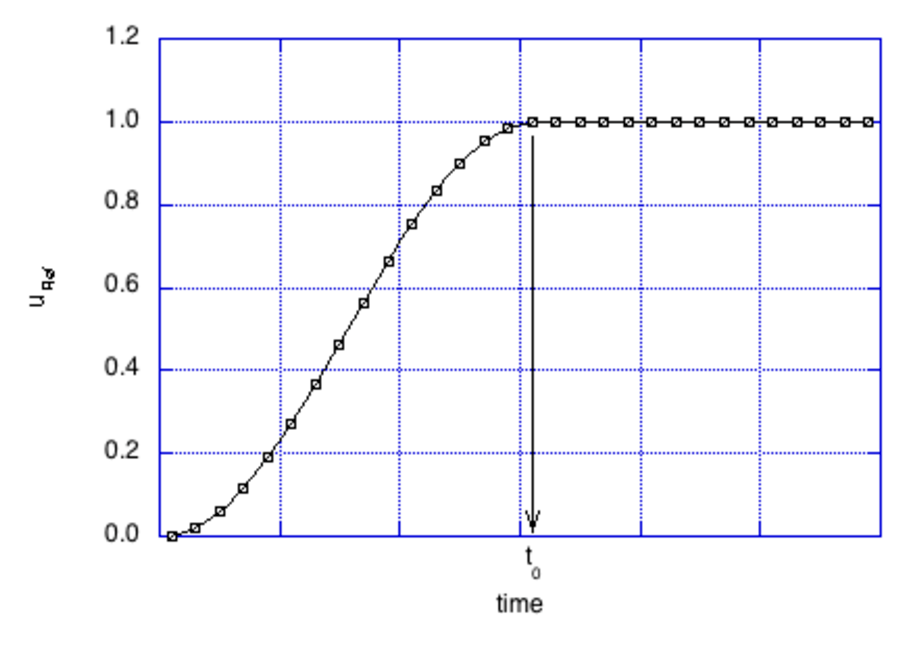
\includegraphics[width=7cm,clip]{accel_Velocity.eps}
\end{center}
\caption{加速中の速度プロファイル}
\label{fig:accel_velocity}
\end{figure}

%
\paragraph{時間積分幅$\Delta{t}$の指定}
\textbf{表\ref{tbl:delta t inc}}に時間積分幅\index{じかんせきぶんはば@時間積分幅}$\Delta{t}$の指定方法を示します.
拡散数\index{かくさんすう@拡散数}$D$は一次元の拡散方程式の場合$D=\alpha \Delta t \slash h^2$で与えられます.$\alpha$は拡散係数で,Navier-Stokes方程式の場合$1/Re$,温度の輸送方程式の場合には$1/Pe$となります.安定性解析から$D<1 \slash 2$であることが要請されます.多次元の場合には,$d_m$を次元数として$\delta t<h^2 \slash (2d_m \alpha)$となります.

Delta\_tにはCFL数\index{CFL},または$\Delta t$を記述します.
時間積分幅の選択は,ソルバの種類を示すKind\_of\_Solverパラメータと関連があり,Solid\_Conductionの場合にはDt\_Directのみ選択できます.

\begin{table}[htdp]
\caption{Time\_Incrementのパラメータ指定}
\begin{center}
\small
\begin{tabular}{lll} \toprule
Dt\_Type & 時間積分幅の決定方法 & Delta\_tへの指定数値\\ \midrule
Direct & $\Delta t$を直接指定する & $\Delta t$\\
%CFL\_DFN\_MaxV & CFL\_MaxVと拡散数により制限される$\Delta t$の値の小さい方を選択\\
%CFL\_DFN\_RefV & CFL\_RefVと拡散数により制限される$\Delta t$の値の小さい方を選択\\
%CFL\_MaxV & CFL数を指定し,瞬時値の最大流速から$\Delta t$を決定 & CFL数\\
CFL\_Reference\_Velocity & CFL数を指定し,代表流速から$\Delta t$を決定 & CFL数\\
Diffusion & 拡散数から$\Delta t$を決定 & |\\
CFL\_Diffusion\_Reference\_Velocity & 代表流速に対するCFL数と拡散数から$\Delta t$を決定 & CFL数\\
%CFL\_MaxV\_CP & CFL数を指定し,音速を考慮した瞬時値の最大流速から$\Delta t$を決定 & CFL数\\
 \bottomrule
\end{tabular}
\end{center}
\label{tbl:delta t inc}
\end{table}



%%%
\pagebreak
\paragraph{計算時間の指定}
Period\_Typeで計算する時間の記述単位を指定します.
計算時間を時間で指定する場合,時間の単位は\hyperlink{tgt:unit}{Unit\_of\_Input\_Parameter}のモードに従います.
指定された単位の数値をCalculation\_Periodで指定します.

\end{indentation}



%%%
\pagebreak
\subsubsection{Treatment\_of\_Wall}

\hypertarget{tgt:treatment_of_wall}{壁面の扱い}について指定します.本パラメータは実験的実装です.

\begin{indentation}{3zw}{0zw}

{\small
\begin{program}
  Treatment_of_Wall {
    Pressure_Gradient = "Grad_Zero"
    Velocity_Profile  = "No_Slip"
  }
\end{program}
}

各パラメータの意味について,\textbf{表\ref{tbl:wall_treatment}}に示します.
圧力勾配は法線方向の圧力勾配ゼロとNavier-Stokes方程式の圧力項を評価する2つの扱いが選択できます\footnote{現時点では,圧力勾配ゼロのみが選択できます.}.
速度プロファイルについては,滑りなし条件と壁関数を用いた近似が選択できます.壁関数は対数則が実装されています.詳細はCBCソルバークラス説明書をご覧ください\footnote{\today 未リリース.}.

\begin{table}[htdp]
\caption{壁面条件の指定}
\begin{center}
\small
\begin{tabular}{lll} \toprule
ラベル & パラメータの値 & 説明\\ \midrule
Pressure\_Gradient & Grad\_Zero & 圧力勾配ゼロ\\
 & Grad\_NS & Navier-Stokes方程式から計算する\\ \hline
Velocity\_Profile  & No\_Slip & 滑りなし壁面条件\\
 & Slip & 滑り壁条件\\
 & Law\_of\_Wall & 壁法則\\ \bottomrule
\end{tabular}
\end{center}
\label{tbl:wall_treatment}
\end{table}

\end{indentation}



%%%
\pagebreak
\subsubsection{Unit}

入力ファイルと出力ファイルで用いる\hypertarget{tgt:unit}{単位を指定}します.

\begin{indentation}{3zw}{0zw}

{\small
\begin{program}
  Unit {
    Unit_of_Input_Parameter = "Non_Dimensional"
    Pressure                = "Gauge"
    Temperature             = "Celsius"
  }
\end{program}
}

各ラベルは,\textbf{表\ref{tbl:param_unit}}に示す単位の指定に用いられます.
有次元のファイル出力時には,圧力単位としてゲージ圧(Gauge Pressure)と絶対圧力(Absolute Pressure)が選択できます.
\textbf{式(\ref{eq:gauge pressure})}に示すゲージ圧を\textbf{式(\ref{eq:ND gauge})}により無次元化する場合に,基準圧として$p_0^\prime\,=\,1.0325\times 10^5$ [Pa]を用い,動圧が$10^0 \sim 10^3$程度とすると,$p \sim \mathrm{O}(1)$程度となるので,単精度計算では4桁程度有効桁が失われる場合もあります.
そのような場合,有次元値のファイル出力単位としてゲージ圧$p_g^\prime$を用います(非圧縮流れの場合には圧力差が意味をもつので,ゲージ圧でもかまいません).
ゲージ圧の基準となる大気圧$p_0^\prime\,$[Pa]は\hyperlink{tgt:reference}{Base\_Pressure}で指定します.
圧力単位の指定は,履歴ファイルのモニタ値にも適用されます.

\begin{equation}
p_g^\prime \,=\, p^\prime \,-\, p_0^\prime
\label{eq:gauge pressure}
\end{equation}

\begin{equation}
p \,=\, \frac{p_g^\prime}{\rho^\prime {u_0^\prime}^2}
\label{eq:ND gauge}
\end{equation}

\begin{table}[htdp]
\caption{単位の指定}
\begin{center}
\small
\begin{tabular}{lll} \toprule
ラベル & 指定パラメータ & 説明\\ \midrule
Unit\_of\_Input\_Parameter & Dimensional or Non\_Dimensional & 入力パラメータファイルの単位を指定します(*1)\\
Pressure & Gauge or Absolute & 入力パラメータの単位が有次元のときに有効となります\\
Temperature & Celsius or Kelvin & 入力パラメータの単位が有次元のときに有効となります\\\bottomrule
\end{tabular}
\end{center}
\label{tbl:param_unit}
\end{table}

\end{indentation}



%%%
\pagebreak
\subsubsection{Version\_Info}

FFV-CソルバーとFlowBaseクラスの\hypertarget{tgt:version}{バージョン番号}を指定します.
異なる番号を指定している場合には,修正すべきバージョン番号が表示されるので入力パラメータファイルを変更します.

\begin{indentation}{3zw}{0zw}
\small
\begin{program}
  Version_Info {
    FFV       = 40
    Flow_Base = 90
  }
\end{program}

\end{indentation}



%%% 隠しパラメータ
\begin{comment}
\subsubsection{Variable\_Range}

温度計算を実施する場合に,変数値を無次元値で[0,1]の範囲に\hypertarget{tgt:variable_range}{制限}することを指定します.

\begin{indentation}{3zw}{0zw}
\small

\begin{program}
<Param name="Variable_Range"     dtype="STRING" value="normal" />
\end{program}

\normalsize
温度の値に制限を課す場合に\textbf{表\ref{tbl:var_range}}に示すパラメータを使用します.保存則を満たさなくなるため,影響を考慮して利用してください.

\begin{table}[htdp]
\small
\caption{Variable\_Rangeのパラメータ指定}
\begin{center}
\begin{tabular}{ll} \toprule
ラベル & モード\\ \midrule
cutoff & 値を無次元で[0, 1]に制限します\\
normal & 制限しません\\ \bottomrule
\end{tabular}
\end{center}
\label{tbl:var_range}
\end{table}

\end{indentation}
\end{comment}


%%%
\pagebreak
\subsection{Parameterセクション}

パラメータセクションでは,FFV-Cソルバーの実行に必要な物理パラメータ\index{ぶつりぱらめーた@物理パラメータ}を記述します.


%%%
\subsubsection{Init\_Temp\_of\_Medium}
温度計算の場合に,割り当てた\hypertarget{tgt:initial_temp}{媒質}に対して初期温度を設定します.


{\small
\begin{program}
  Init_Temp_of_Medium {
    air-100c      = 72.0
    Al-insulator  = 72.0
    Fe-heat_src_1 = 100.0
    Fe-heat_src_2 = 500.0
    Fe-heat_src_3 = 150.0
    Fe-heat_src_4 = 400.0
    Fe-heat_src_5 = 340.0
  }
\end{program}
}



%%%
\pagebreak
\subsubsection{Intrinsic\_Example}

\hypertarget{tgt:intrinsic_example}{組み込み}例題\index{くみこみれいだい@組み込み例題}に固有のパラメータを指定します.

\begin{indentation}{3zw}{0zw}
\small

\begin{program}
  Intrinsic_Example {
    fluid_medium = "air"
    solid_medium = "fe"
  }
\end{program}

\normalsize
指定可能なパラメータは,\textbf{表\ref{tbl:intrinsic_parameter}}に示すように各\hyperlink{tgt:example}{組み込み例題}ごとに異なります.

\begin{table}[htdp]
\caption{Intrinsic\_Exampleセクションで指定できるパラメータ}
\begin{center}
\small
\begin{tabular}{llll} \toprule
組み込み例題 & 指定パラメータラベル & dtype & 指定値\\ \midrule
Duct & Shape     & STRING & Circular, Rectangular\\
     & Diameter  & REAL   & 断面径 [m]\\
     & Direction & STRING & X\_minus $|$ X\_plus $|$ Y\_minus $|$ Y\_plus $|$ Z\_minus $|$ Z\_plus\\
     & Driver    & REAL   & ドライバ部分の長さ [m]\\ \bottomrule
\end{tabular}
\end{center}
\label{tbl:intrinsic_parameter}
\end{table}

\end{indentation}



%%%
\pagebreak
\subsubsection{Reference}

解析に用いる無次元化の\hypertarget{tgt:reference}{基準量},あるいは無次元パラメータを指定します.

\begin{indentation}{3zw}{0zw}

{\small
\begin{program}
  Reference {
    Length        = 1.0
    Velocity      = 1.0
    Gravity       = 9.8
    Base_Pressure = 0.0
    Reynolds      = 1000.0
    Prandtl       = 0.71
    Base_Medium   = "air"
  }
\end{program}
}

\noindent \textbf{表\ref{tbl:ref_value}}に示すように基準量を必要に応じて記述できます.
無次元パラメータであるReynolds数とPrandtl数は,\hyperlink{tgt:unit}{Unit}の指定が無次元のときのみ指定できます.
Base\_Mediumで指定する名前は,モデル内で使われている必要があります.
固体熱伝導解析の場合には固体のラベルを指定し,それ以外の(熱)流動解析の場合には流体のラベルを指定します.

\begin{table}[htdp]
\caption{Referenceセクションで指定できるパラメータ}
\begin{center}
\small
\begin{tabular}{llll} \toprule
値 & 意味 & 単位\\ \midrule
Length & 代表長さ & $m$ &\\
Velocity & 代表速度 & $m/s$ &\\
Base\_Pressure & 基準圧力 & $Pa$ &\\
Gravity & 重力加速度 & $m^2/s$ &\\
%Grashof & グラショフ数 & |\\
Prandtl & プラントル数 & | & 無次元のときのみ指定\\
%Rayleigh & レイリー数 & |\\
Reynolds & レイノルズ数 & | & 無次元のときのみ指定\\
Base\_Medium & 代表物性値として指定する媒質ラベル & | &\\ \bottomrule
\end{tabular}
\end{center}
\label{tbl:ref_value}
\end{table}

\end{indentation}



%%%
\pagebreak
\subsubsection{Temperature}

\hypertarget{tgt:temperature}{温度計算}を実施する場合の基準量を有次元値で指定します.

\begin{indentation}{3zw}{0zw}

{\small
\begin{program}
  Temperature {
    Base       = 20.0
    Difference = 35.0
  }
\end{program}
}

基準温度(Base)と温度差(Difference)は,非圧縮計算のパッシブスカラーによる温度計算では温度場を特徴づける代表量となります.
単位は\hyperlink{tgt:unit}{Temperature}ラベルで指定します.

\end{indentation}



%%%
\pagebreak
\subsection{Medium\_Tableセクション}

ソルバーで利用する媒質の\hypertarget{tgt:medium_table}{物性値テーブル}を記述します.
ここで記述する媒質の基本リスト\index{きほんりすと@基本リスト!ばいしつの@媒質の---}は,解析に利用される候補です.
媒質は流体と固体が記述でき,\textbf{表\ref{tbl:MTLentry}}により媒質を指定します.

\begin{indentation}{3zw}{0zw}

{\small
\begin{program}
Medium_Table {

  Medium[@] {
    type                 = "Fluid"
    label                = "Air"
    Density              = 1.1763
    Specific_Heat        = 1007
    Thermal_Conductivity = 2.614e-02
    Kinematic_Viscosity  = 15.83e-06
    Viscosity            = 18.62e-06
    Sound_of_Speed       = 340.0
    volume_expansion     = 0.04e-3 
  }

  Medium[@] {
    type                 = "Solid"
    label                = "Fe"
    Density              = 7870.0
    Specific_Heat        = 442.0
    Thermal_Conductivity = 80.3
  }

}
\end{program}
}

\begin{table}[htdp]
\caption{Medium\_Tableに記述するパラメータ}
\begin{center}
\begin{tabular}{ll} \toprule
ラベル & 説明\\ \midrule
Type & Fluid または Solid\\
Label & 媒質名\\ \bottomrule
\end{tabular}
\end{center}
\label{tbl:MTLentry}
\end{table}


各媒質は固体と流体によって記述しなければならない物性値が異なります.
指定できる項目を\textbf{表\ref{tbl:medium_tbl}}に示します.
固体については,密度・比熱・熱伝導率のみの記述となります.
各媒質の情報は,任意に指定するID番号によって管理されます.

\begin{table}[htdp]
\caption{Medium\_Tableにおける物性値の指定}
\begin{minipage}{.45\textwidth}
\begin{center}
\begin{tabular}{lll}\\ \toprule
Fluidのラベル & 説明 & 単位\\ \midrule
Density & 密度 & $kg/m^3$\\
Specific\_Heat & 定圧比熱 & $kJ/(kg K)$\\
Thermal\_Conductivity & 熱伝導率 & $W/(m K)$\\
Kinematic\_Viscosity & 動粘性係数 & $m^2/s$\\
Viscosity & 粘性係数 & $Pa\,s$\\
Sound\_of\_Speed & 音速 & $m/s$\\
Volume\_Expansion & 体膨張率 & $1/K$\\ \bottomrule
\end{tabular}
\end{center}
\end{minipage} \hfill
\begin{minipage}{.45\textwidth}
\begin{center}
\begin{tabular}{lll}\\ \toprule
Solidのラベル & 説明 & 単位\\ \midrule
Density & 密度 & $kg/m^3$\\
Specific\_Heat & 定圧比熱 & $kJ/(kg K)$\\
Thermal\_Conductivity & 熱伝導率 & $W/(m K)$\\ \bottomrule
\end{tabular}
\end{center}
\end{minipage}
\label{tbl:medium_tbl}
\end{table}

\end{indentation}





%%%
\chapter{境界条件}

\begin{abstract}
本章では,FFV-Cソルバーで設定できる境界条件の設定について説明します.
まず境界条件と媒質を指定するパラメータの構造について述べた後,流れと熱の境界条件について説明します.
\end{abstract}
%
\graphicspath{{./fig_BC/}}

%
\section{境界条件の概要}

%
\hypertarget{tgt:BC policy}{\subsection{外部境界条件と局所境界条件}}
FFV-Cソルバーでは,境界条件を外部境界条件と局所境界条件の2つに分けて指定します.
外部境界条件は計算領域外部面に指定する境界条件で,局所境界条件は計算領域内部に指定する境界条件です.
\textbf{図\ref{fig:BCs}}に示すように,計算領域を構成する6面が外部境界面で,この部分に与える境界条件が外部境界条件です.
それ以外の内部領域(セル体積とセルフェイス)に作用する境界条件は局所境界条件として扱います.
外部境界面には,外部境界条件が各面に対して1種類のみ与えることができ,局所境界条件を部分的に適用することができます.

\begin{figure}[htbp]
\begin{center}
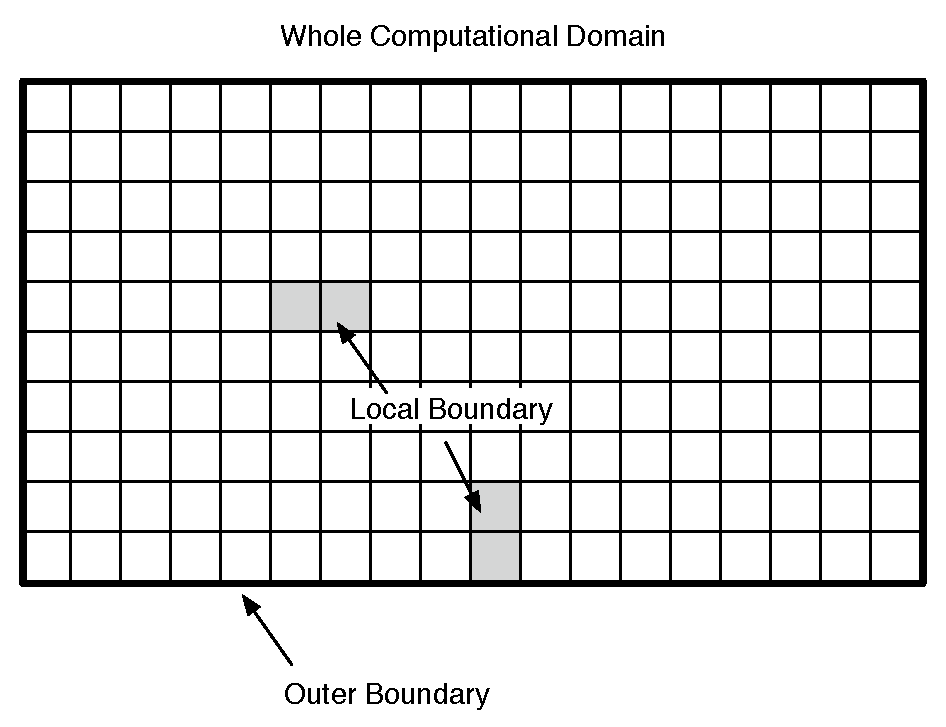
\includegraphics[width=10cm,clip]{Boundary.eps}
\end{center}
\caption{計算領域における外部境界と局所境界の指定場所}
\label{fig:BCs}
\end{figure}


%
\subsection{BC\_Tableセクションのパラメータ構造}

BC\_Tableセクションでは,次のように局所境界条件LocalBoundary\index{LocalBoundary}と外部境界条件OuterBoundary\index{OuterBoundary}の2つを記述します.

{\small
\begin{program}
BC_Table {

  LocalBoundary {
    specified_velocity {
      suction {
        type           = "velocity"
        profile        = "constant"
        velocity       = 3.0
        Normal         = (0.0, 0.0, -1.0)
        BC_direction   = "opposite"
        //frequency      = 0.0 //REAL
        //initial_phase  = 0.0 //REAL
        //constant_bias  = 0.0 //REAL
        temperature    = 35.0 //REAL
      }
    }

    Pressure_Loss {
      radiator1 {
        "normal" = (1.0, 0.0, 0.3) //REAL
        "dir[@]" = (0.0, 1.0, 0.0) //REAL
        "center" = (6.0, 1.6, 0.3) //REAL
        "depth" = 0.2 //REAL
        "width" = 2.0 //REAL
        "height" = 1.0 //REAL
        "c" = (1.0, 0.0, 0.0, 0.8) //REAL
        "u_threshold" = 0.2 //REAL
        "thickness" = 80.0 //REAL
        "unit" = "non_dimension" //STRING
        "vector" = "directional" //STRING
      }
    }
      "Fan"{
        "fan"{
          "normal" = (1.0, 1.0, 0.0) //REAL
          "center" = (5.0, 1.0, 0.5) //REAL
          "depth" = 0.3 //REAL
          "fan_radius" = 1.0 //REAL
          "boss_radius" = 0.5 //REAL
          "unit" = "non_dimension" //STRING
        }
      }
      "Cell_Monitor"{
        "sensor"{
          "shape" = "cylinder" //STRING
          "normal" = (0.0, 0.0, -1.0) //REAL
          "center" = (0.0, 0.0, -0.198) //REAL
          "depth" = 0.01 //REAL
          "radius" = 0.022 //REAL
          "Sampling_Method" = "nearest" //STRING
          "Sampling_Mode" = "Fluid" //STRING
          "Variables[@]"= "velocity"
          "Variables[@]"= "pressure"
          //"Variables[@]"= "temperature" //commentout = off
          "Variables[@]"= "total_pressure"
        }
      }
  } //LocalBoundary

  OuterBoundary {
      
    // 境界条件候補リスト
    Basic_BCs[@] {
      alias    = "outer_wall"
      class    = "Wall"
      Type     = "fixed"
    }
    Basic_BCs[@] {
      alias    = "slide_wall"
      class    = "wall"
      Type     = "slide"
      Profile  = "Constant"
      Normal   = (1.0, 0.0, 0.0)
      Velocity = 1.0
    }
    Basic_BCs[@] {
      alias    = "inlet_2"
      class    = "Specified_Velocity"
      Profile  = "Constant"
      Normal   = (1.0, 0.0, 0.0)
      velocity = 5.0
    }
    Basic_BCs[@] {
      alias    = "outflow_1"
      class    = "Outflow"
      velocity_Type = "Average"
    }
      
    //外部境界条件
    Face_BC {
      X_minus {
        kind   = "inlet_2"
        medium_on_guide_cell = "air"
      }
      X_plus {
        kind   = "outflow_1"
        medium_on_guide_cell = "air"
      }
      Y_minus {
        kind   = "outer_wall"
        medium_on_guide_cell = "Fe"
      }
      Y_plus {
        kind   = "outer_wall"
        medium_on_guide_cell = "Fe"
      }
      Z_minus {
        kind   = "outer_wall"
        medium_on_guide_cell = "Fe"
      }
      Z_plus {
        kind   = "slide_wall"
        medium_on_guide_cell = "Fe"
      }
    }

  } // OuterBoundary

} // BC_Table
\end{program}
}


%
\subsection{OuterBoundary}

\hypertarget{tgt:outer_boundary}{計算領域の外部境界条件}を次の方針により指定します.

\begin{enumerate}
\item 候補となる境界条件の種類をBasic\_BCsタグ内にリストアップし,基本リストを作成します.境界条件の基本リスト\index{きほんりすと@基本リスト!きょうかいじょうけんの@境界条件の---}には,classに\textbf{表\ref{tbl:outer BC physical}}に示すキーワードを与え,aliasにユニークなラベルを与えます.
\item Face\_BCタグ内において,境界条件の基本リストのaliasラベルを参照してkindラベルに指定し,計算領域の外部境界の各面における境界条件を指定します.同時に,各面のガイドセルのセルIDをmedium\_on\_guide\_cellにより指定します.
\end{enumerate}

前述の例では,境界条件の候補として\verb|class=Wall, Specified_Velocity, Outflow|の3種類がリストアップされています.
Xマイナス方向の外部境界面に流入条件(inlet\_2)を与え,Xプラス方向の外部境界面に流出境界条件(outflow\_1),それ以外の面には壁面条件(outer\_wall, slide\_wall)を与えています.
各外部境界面のガイドセルにはmedium\_on\_guide\_cellによって,媒質をラベルで付与しています.
このラベルは,\hyperlink{tgt:medium_table}{Medium\_Table}セクションにリストアップされた媒質ラベルを参照します.
外部境界条件は,計算領域を構成する外部境界面の各面ごとに一様な境界条件となります.

指定できる境界条件の種類を\textbf{表\ref{tbl:outer BC physical}}に示します.
熱流れの場合には,壁面境界の場合に細かい指定が可能です.

\begin{table}[htdp]
\caption{外部境界で指定できる流れと熱の境界条件の種類}
\begin{center}
\small
\begin{tabular}{ll|ll} \toprule
流れの境界指定のラベル名 &  流れの境界条件 & 熱境界指定のラベル名 & 熱境界条件\\ \midrule
Outflow & 流出境界 & $\leftarrow$ & 対流流出\\
Periodic & 周期境界 & $\leftarrow$ & 周期境界\\
Specified\_Velocity & 流入境界 & Temperature & 流入温度指定\\
Symmetric & 対称境界 & $\leftarrow$ & 対称境界\\
Traction\_Free & 遠方境界 & Ambient\_Temperature & 遠方温度指定\\
Far\_Field & 遠方境界 & Ambient\_Temperature & 遠方温度指定 *テスト実装\\ \hline
Wall & 壁面境界 & Adiabatic & 断熱指定\\
& & HeatFlux & 熱流束指定\\ 
& & HeatTransfer Type\_S & 熱伝達係数と表面温度から熱伝達を計算\\
& & HeatTransfer Type\_SF & 強制対流の層流・乱流熱伝達境界\\
& & HeatTransfer Type\_SN & 自然対流の乱流熱伝達境界\\
& & HeatTransfer Type\_B & 固体壁からの放熱条件\\
& & IsoThermal & 等温指定\\
\bottomrule
\end{tabular}
\end{center}
\label{tbl:outer BC physical}
\end{table}


%
\pagebreak
\subsection{LocalBoundary}

\hypertarget{tgt:localboundary}{計算領域内に存在する局所的な境界条件}を記述するセクションで,\textbf{表\ref{tbl:tag_ibc}}に示す種類を指定できます.
FFV-Cソルバーは,局所境界条件をコンポーネント\index{コンポーネント}として扱います.
局所境界条件を指定する位置には,セル要素に対して作用するものとセル界面に作用する2種類のコンポーネントがあります.

局所境界条件の位置と形状は,解析幾何形状モデルに与えられたラベルにより判断します.
また,境界条件の詳細は,LocalBoundaryセクションの対応するラベルに記述します.
局所境界条件で指定する各コンポーネントの個数と実際の解析モデル中のコンポーネントの個数は一致している必要があります.
\textbf{指定できる局所境界条件の数は30個が上限}です.
また,\textbf{指定境界条件数と媒質数の和は30個以下}となります\footnote{これらの制限は,境界条件を効率よく実装する方法の制約から来るものです.}.

Inactiveタグは,計算空間内で計算しない不活性セルを指定します.
Cell\_Monitorは境界条件ではありませんが,境界条件と同じ指定方法を用いて実装しているので,このセクションに設けています.


\begin{table}[htdp]
\caption{局所境界条件(コンポーネント)の種類}
\begin{center}
\small
\begin{tabular}{lllll} \toprule
ラベル名 & 指定位置 & 計算モード & 実装形式 & コンポーネントの説明\\ \midrule
Specified\_Velocity & セル界面 & 流れ・熱流れ & 対流流束 & 速度指定境界\\
Outflow & セル界面 & 流れ・熱流れ & 対流流束 & 流出境界\\
Periodic & セル界面 & 流れ・熱流れ & 参照値指定 & 部分周期境界\\
%FORCING & Direct ForcingによるImmersed Boundary境界条件\\
%HEX & 熱交換器\\
%FAN & ファン\\
%DARCY & ダルシー則\\
Inactive & セル要素 & 流れ・熱流れ & マスク & 不活性化する計算空間内のセルIDを指定\\
Cell\_Monitor & セル要素 & 流れ・熱流れ & - & 物理量のモニター位置の指定\\ 
Adiabatic & セル界面 & 熱流れ & 熱流束マスク & 断熱セル指定\\
Direct\_Heat\_Flux & セル界面 & 熱流れ & 熱流束 & 熱流束指定\\
HeatTransfer\_B & セル界面 & 固体伝熱 & 熱流束 & 固体壁からの放熱条件\\
HeatTransfer\_S & セル界面 & 熱流れ & 熱流束 & 熱伝達係数と表面温度により計算\\
%HeatTransfer\_N & セル界面 & 熱 & 熱流束 & 熱伝達形式\\
HeatTransfer\_SF & セル界面 & 熱流れ & 熱流束 & 強制対流の層流・乱流熱伝達境界\\
HeatTransfer\_SN & セル界面 & 熱流れ & 熱流束 & 自然対流の乱流熱伝達境界\\
IsoThermal & セル界面 & 熱流れ & 熱流束 & 等温面指定\\
Heat\_Source & セル要素 & 熱流れ & 外力項 & 吸発熱指定\\
Specified\_Temperature & セル要素 & 熱流れ & 温度指定 & セルの温度指定\\
\bottomrule
\end{tabular}
\end{center}
\label{tbl:tag_ibc}
\end{table}


%
\pagebreak
\subsection{計算格子と内部・外部領域}

非圧縮性流体の境界条件で参照する\hypertarget{tgt:grid_arrangement}{計算領域と格子配置}について説明します.
計算領域とコロケート変数配置\index{へんすうはいち@変数配置!コロケート@Collocated---}の変数のインデクス\index{インデクス}の表記を\textbf{図\ref{fig:index_domain}},\textbf{図\ref{fig:index_cc}}に示します.

\begin{figure}[htdp]
  \begin{center}
  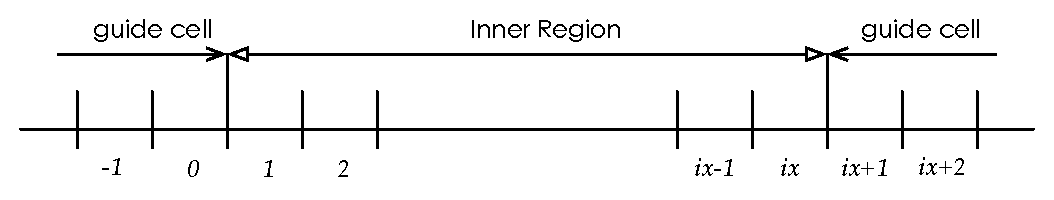
\includegraphics[width=12cm,clip]{index_domain.eps}
  \end{center}
  \caption{計算領域のインデクス}
  \label{fig:index_domain}
\end{figure}

\begin{figure}[htdp]
  \begin{center}
  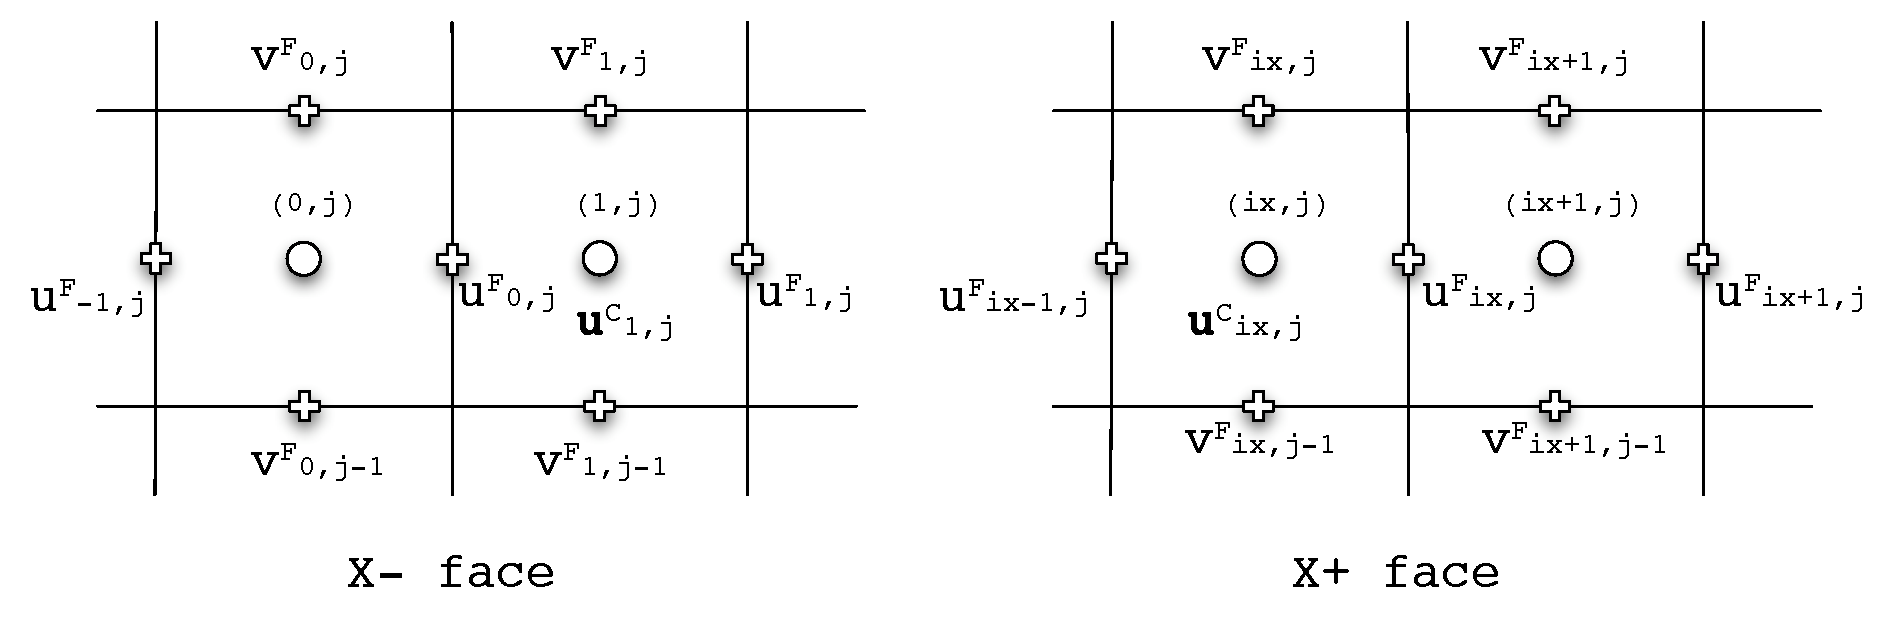
\includegraphics[width=14cm,clip]{index_cc.eps}
  \end{center}
  \caption{コロケート配置の変数のインデクス.基本変数($u_{\,i}^{\,C},\, p,\,\theta$)は全てセルセンタ位置に配置され,補助的な速度ベクトル$u_{\,i}^{\,F}$がスタガード位置に配置されます.}
  \label{fig:index_cc}
\end{figure}



%%%
\pagebreak
\section{外部境界条件}

%
\subsection{壁面境界}

\subsubsection{流れの境界条件}

壁面の速度境界条件では,指定する境界面の移動速度を与えます.
壁面速度が時間的に変化する場合と一定の場合があります.
ただし,壁面速度ベクトルは壁面と平行なスライド成分のみで,壁面と垂直な成分はゼロである点に注意します.

壁面境界は,与えられた速度からセルフェイス位置の運動量流束を計算して,運動量流束を直接与えます.
外部境界では下記のような入力パラメータで指定します.
次の境界条件の例では,Y方向に7[m/s],2[Hz]で平行振動する壁の境界条件を指定しています.

{\small
\begin{program}
OuterBoundary {
  Basic_BCs[@] {
    alias    = "inlet_2"
    class    = "Specified_Velocity"
    Profile  = "Harmonic"
    Normal   = (0.0, 1.0, 0.0)
    amplitude= 7.0
    frequency= 2.0
    initial_phase = 0.0
    constant_bias = 0.0
  }
}
\end{program}
}

\begin{table}[htdp]
\caption{壁面の速度境界条件の指定パラメータ}
\begin{center}
\small
\begin{tabular}{lll} \toprule
ラベル & 指定ラベル名 & パラメータの説明\\ \midrule
Normal & | & 法線ベクトルの成分\\
Profile & Constant $|$ Harmonic & 指定速度のタイプ\\
Velocity & | & 指定単位 $[m/s]$,Profile=constantの場合のみ\\
Amplitude & | & 速度,以下のパラメータはProfile=harmonicの場合のみ\\
Frequency & | & 周波数 $f\, [Hz]$\\
Initial\_Phase & | & 初期位相 $\phi\, [Rad]$\\
Constant\_Bias & | & 一定値 $b\, [m/s]$\\
\bottomrule
\end{tabular}
\end{center}
\label{tbl:wall parameter out}
\end{table}

壁面の速度境界の指定パラメータを\textbf{表\ref{tbl:wall parameter out}}に示します.
時間変化を伴う速度指定はProfile=\lq\lq Harmonic\rq\rq を指定し,\textbf{式(\ref{eq:harmonic out})}の形式の単振動\index{たんしんどう@単振動}の境界条件を周期や初期位相,固定バイアスと供に与えます.時間的に変化しない壁面境界の場合にはProfile=\lq\lq Constant\rq\rq を指定し,周波数,初期位相,固定バイアス値の指定は不要です.

\begin{equation}
V \,{=}\, A \sin \left( 2 \mathrm{\pi} ft \,+\, \phi \right) \,+\, b
\label{eq:harmonic out}
\end{equation}


壁面境界に対する圧力の境界条件は,Navier-Stokes方程式からNeumann型の圧力境界条件が得られます.
高レイノルズ数流れにおいては,粘性項の寄与が小さいと仮定し粘性項を省略し$\nabla p=0$の形式になります.
圧力の壁面境界条件については,内部と外部の扱いは同じで,スキーム中で壁面を認識し$\nabla p=0$が満たされるようになっていますので,明示的な境界条件の指定は必要ありません.

%
\subsubsection{熱境界条件}
計算領域の外部面における壁面に対する熱境界条件としては,断熱,熱流束,熱伝達,等温が指定できます.
熱伝達境界は,さらに幾つかの指定パターンがあります.
詳細はInside\_FFVC.pdfをご覧ください.

%
\paragraph{断熱境界}
熱流束がゼロ,つまり$q^{\prime}=0$を指定します.
下記の例では,固定壁(壁面速度がゼロ)で,断熱条件を指定しています.

{\small
\begin{program}
<OuterBoundary>
  <Elem name="Basic_BCs">
    <Elem name="wall" id="1">
      <Param name="Normal_x"        dtype="REAL"   value="0.0" />
      <Param name="Normal_y"        dtype="REAL"   value="1.0" />
      <Param name="Normal_z"        dtype="REAL"   value="0.0" />
      <param name="Profile"         dtype="STRING" value="Constant" />
      <param name="Specified_Type"  dtype="STRING" value="Velocity" />
      <Param name="Specified_Value" dtype="REAL"   value="0.0" />
      <Param name="Heat_Type"       dtype="STRING" value="Adiabatic" />
    </Elem>
  </Elem>
</OuterBoundary>
\end{program}
}

%
\paragraph{熱流束境界}
境界面で指定の熱流束$q^{\prime}[W/m^2]$を与えます.
符号は計算領域内に流入する熱流束の場合に正,流出する熱流束の場合に負とします.
下記の例ではid=1の条件として,$12.0[W/m^2]$で流入する熱流束をもつ面を指定しています.

{\small
\begin{program}
<OuterBoundary>
  <Elem name="Basic_BCs">
    <Elem name="wall" id="1">
      ...
      <Param name="Heat_Type"       dtype="STRING" value="HeatFlux" />
      <Param name="Heat_Flux"       dtype="REAL"   value="12.0" />
    </Elem>
  </Elem>
</OuterBoundary>
\end{program}
}


%
\hypertarget{tgt:heat-transfer}{\paragraph{熱伝達境界}}
熱伝達境界は次式の形式で熱流束を与える条件で,幾つかの種類があります.
熱流体解析のモードと指定できる熱伝達境界の関係を\textbf{表\ref{tbl:type of HT}}に示します.

\begin{table}[htdp]
\caption{熱伝達境界条件とKind\_of\_Solverの関係}
\begin{center}
\small
\begin{tabular}{ll} \toprule
KIND\_OF\_SOLVER & 指定できる熱伝達境界の種類\\ \midrule
FLOW\_ONLY & -\\
THERMAL\_FLOW $|$ THERMAL\_FLOW\_NATURAL & Type\_S $|$ Type\_SN $|$ Type\_SF\\
CONJUGATE\_HEAT\_TRANSFER & Type\_N\\
SOLID\_CONDUCTION & Type\_B\\ \bottomrule
\end{tabular}
\end{center}
\label{tbl:type of HT}
\end{table}


\begin{equation}
q^{\prime} \,=\, -H(\theta_{sf}^{\prime}\,-\,\theta_{\infty}^{\prime})
\label{eq:ht form}
\end{equation}

\begin{center}
\begin{tabular}{lll}
$H$ &  $[W\,/\,(m^2K)]$ & Coefficient\, of\, heat\, transfer\\
$\theta_{sf}^{\prime}$ & $[K]$ & Surface\, temperature\, of\, solid\\
$\theta_{\infty}^{\prime}$ & $[K]$ & Temperature\, at\, outer\, boundary\, layer\\
\end{tabular}
\end{center}

\vspace{5mm}
\begin{indentation}{3zw}{0zw}

%
\subparagraph{Type\_S  表面温度と熱伝達係数により計算}
Type\_Sは表面温度と熱伝達係数を与え,熱流束を計算します.
\textbf{式(\ref{eq:ht form})}において,熱伝達係数$H$と固体表面温度$\theta_{sf}^{\prime}$を与え,\textbf{図\ref{fig:HT_Type_S}}に示す固体表面に隣接する流体セルの値を$\theta_{\infty}^{\prime}$として,界面での熱流束を計算します.

\begin{figure}[htdp]
\begin{center}
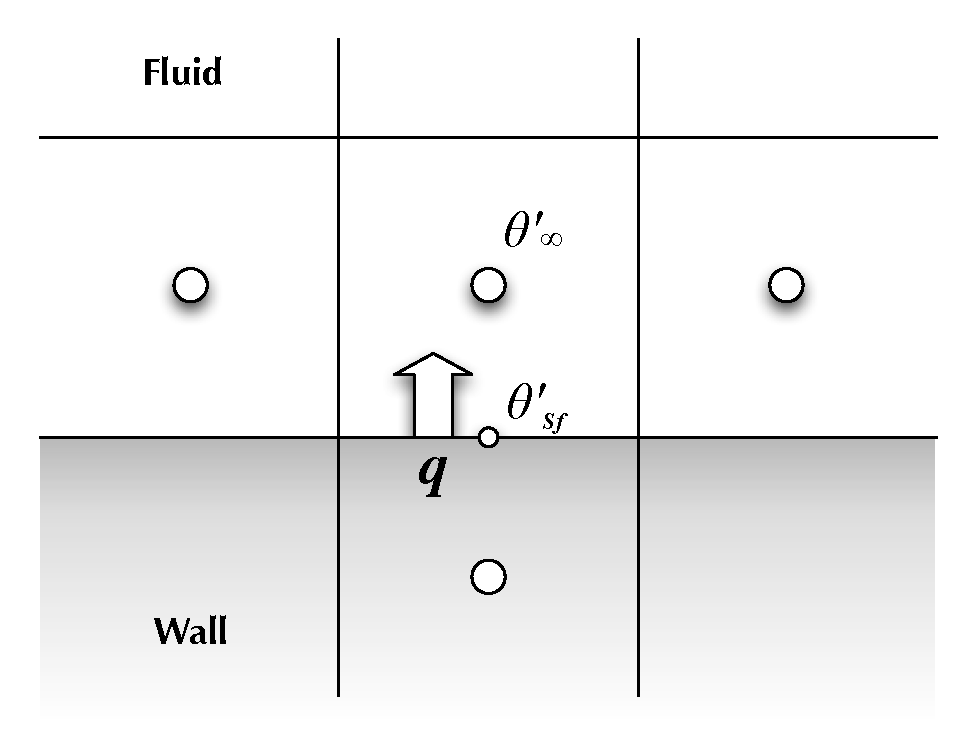
\includegraphics[width=7cm,clip]{HeatTransfer_Type_S.eps}
\end{center}
\caption{Type\_Sの熱伝達境界}
\label{fig:HT_Type_S}
\end{figure}

以下に,熱境界部分のみパラメータ指定の一例を示します.

{\small
\begin{program}
<OuterBoundary>
  <Elem name="Basic_BCs">
    <Elem name="wall" id="1">
      ...
      <Param name="Heat_Type"             dtype="STRING" value="HeatTransfer_S" />
      <Param name="Surface_Temperature"   dtype="REAL"   value="300.0"/>
      <Param name="Coef_of_Heat_Transfer" dtype="REAL"   value="20.0"/>
    </Elem>
  </Elem>
</OuterBoundary>
\end{program}
}

\begin{table}[htdp]
\caption{熱伝達境界Type\_Sの指定パラメータ}
\begin{center}
\small
\begin{tabular}{ll} \toprule
指定キーワード & パラメータの説明\\ \midrule
Coef\_of\_Heat\_Transfer & 熱伝達係数$[W/(m^2K)]$\\
Surface\_Temperature & 表面温度$[K\,|\,{}^\circ\mathrm{C}]$\\
\bottomrule
\end{tabular}
\end{center}
\label{tbl:hts}
\end{table}

%
\subparagraph{Type\_SN  自然対流の乱流熱伝達}
自然対流の場合の乱流熱伝達の実験式を実装した境界条件です.
文献\cite{shouji:95:Dennetsu}には,平板に対する自然対流の層流と乱流の熱伝達に関する近似式が説明されています.
雰囲気流体の温度に比べ加熱面の温度が非常に高い場合,平板が長くなると境界層が不安定になり,ほぼ$Ra>10^9$で層流から乱流へ遷移します.
垂直平板に関する平均熱伝達$(\overline{Nu_L},代表長L)$は次式で整理されます.

\begin{equation}
\left.
\begin{array}{lll}
\vspace{1mm}
層流 & \overline{Nu_L} \,=\, 0.59Ra_L^{1/4} & (10^4 < Ra_L < 10^9)\\
乱流 & \overline{Nu_L} \,=\, 0.10Ra_L^{1/3} & (10^9 < Ra_L < 10^{13})
\end{array} \right\}
\label{eq:natural_convection_vert_ht}
\end{equation}

一方,水平平板の場合には,加熱面が上面と下面にある場合で雰囲気流体の挙動が異なるため,\textbf{式(\ref{eq:natural_convection_horiz_ht})}のように整理されています.

\begin{equation}
\left.
\begin{array}{lll}
\vspace{1mm}
上面加熱 & \overline{Nu_L} \,=\, 0.54Ra_L^{1/4} & (10^4 < Ra_L < 10^7)\\
\vspace{1mm}
上面加熱 & \overline{Nu_L} \,=\, 0.15Ra_L^{1/3} & (10^7 < Ra_L < 10^{11})\\
\vspace{1mm}
下面加熱 & \overline{Nu_L} \,=\, 0.27Ra_L^{1/4} & (10^5 < Ra_L < 10^{10})
\end{array} \right\}
\label{eq:natural_convection_horiz_ht}
\end{equation}

上式を形式的にまとめると,

\begin{equation}
H \,=\, \alpha Ra_L^\beta \frac{\lambda}{L^\prime}
\label{eq:typeSN_form_ht}
\end{equation}

Type\_SNの境界条件は,上式のパラメータを実装しています.ここでは,垂直平板と水平平板の上面は,同じ係数を用いています.

{\small
\begin{program}
<OuterBoundary>
  <Elem name="Basic_BCs">
    <Elem name="wall" id="1">
      ...
      <Param name="Heat_Type"                dtype="STRING" value="HeatTransfer_SN" />
      <Param name="Surface_Temperature"      dtype="REAL"   value="500.0"/>
      <Param name="Ref_Temp_Mode"            dtype="STRING" value="Bulk_Temperature"/>
      <Param name="vertival_laminar_alpha"   dtype="REAL"   value="0.59"/>
      <Param name="vertival_laminar_beta"    dtype="REAL"   value="0.25"/>
      <Param name="vertival_turbulent_alpha" dtype="REAL"   value="0.1"/>
      <Param name="vertival_turbulent_beta"  dtype="REAL"   value="0.3333333"/>
      <Param name="vertival_ra_critial"      dtype="REAL"   value="1.0e9"/>
      <Param name="lower_laminar_alpha"      dtype="REAL"   value="0.27"/>
      <Param name="lower_laminar_beta"       dtype="REAL"   value="0.25"/>
      <Param name="lower_turbulent_alpha"    dtype="REAL"   value="0.27"/>
      <Param name="lower_turbulent_beta"     dtype="REAL"   value="0.25"/>
      <Param name="lower_ra_critial"         dtype="REAL"   value="1.0e9"/>
    </Elem>
  </Elem>
</OuterBoundary>
\end{program}
}

\begin{table}[htdp]
\caption{熱伝達境界Type\_SNのパラメータ}
\begin{center}
\small
\begin{tabular}{ll}\toprule
パラメータタグ & 記号の意味\\ \midrule
Vertival\_Laminar\_Alpha & 垂直平板と水平平板(上面)の層流時の係数$\alpha$\\
Vertival\_Laminar\_Beta & 垂直平板と水平平板(上面)の層流時の係数$\beta$\\
Vertival\_Turbulent\_Alpha & 垂直平板と水平平板(上面)の乱流時の係数$\alpha$\\
Vertival\_Turbulent\_Beta & 垂直平板と水平平板(上面)の乱流時の係数$\beta$\\
Vertival\_Ra\_Critial & 垂直平板と水平平板(上面)の臨界Ra数$Ra_L$\\
Lower\_Laminar\_Alpha & 水平平板(下面)の層流時の係数$\alpha$\\
Lower\_Laminar\_Beta & 水平平板(下面)の層流時の係数$\beta$\\
Lower\_Turbulent\_Alpha & 水平平板(下面)の乱流時の係数$\alpha$\\
Lower\_Turbulent\_Beta & 水平平板(下面)の乱流時の係数$\beta$\\
Lower\_Ra\_Critial & 水平平板(下面)の臨界Ra数$Ra_L$\\ 
Ref\_Temp\_Mode & Bulk\_Temperature or Local\_Temperature\\ \bottomrule
\end{tabular}
\end{center}
\label{tbl:htsn}
\end{table}


%
\subparagraph{Type\_SF  強制対流の層流・乱流熱伝達}
強制対流の場合の層流・乱流熱伝達の実験式を実装した境界条件です.
文献\cite{shouji:95:Dennetsu}から,平板に対する発達した強制対流の乱流熱伝達は,実験による摩擦係数の測定結果とチルトン-コルバーンのアナロジーを用い,温度一定で平板が遷移長さよりも十分に大きいと仮定すると,\textbf{式(\ref{eq:forced_convection_ht})}のように表せます.
実験式を整理すると,熱伝達係数は以下のような表現ができます.

\begin{equation}
\overline{Nu_L} \,=\, 0.037Re_L^{4/5}Pr^{1/3}
\label{eq:forced_convection_ht}
\end{equation}

形式的に次式のように表し,パラメータを求めます.

\begin{equation}
H \,=\, \alpha Re_L^\beta \, Pr^\gamma \, \frac{\lambda}{L^\prime}
\label{eq:typeSF_form_ht}
\end{equation}


温度差の定義にはバルク温度と隣接セルの値を用いたオプションが選択できます.
以下に,パラメータ指定の一例を示します.

{\small
\begin{program}
<OuterBoundary>
  <Elem name="Basic_BCs">
    <Elem name="wall" id="1">
      ...
      <Param name="Heat_Type"           dtype="STRING" value="HeatTransfer_SF" />
      <Param name="Surface_Temperature" dtype="REAL"   value="500.0"/>
      <Param name="Ref_Temp_Mode"       dtype="STRING" value="Bulk_Temperature"/>
      <Param name="alpha"               dtype="REAL"   value="0.037"/>
      <Param name="beta"                dtype="REAL"   value="0.8"/>
      <Param name="gamma"               dtype="REAL"   value="0.333333"/>
    </Elem>
  </Elem>
</OuterBoundary>
\end{program}
}

\begin{table}[htdp]
\caption{熱伝達境界Type\_SFのパラメータ}
\begin{center}
\small
\begin{tabular}{ll}\toprule
タグ & 記号の意味\\ \midrule
alpha & \textbf{式(\ref{eq:typeSF_form_ht})}中の係数$\alpha$\\
beta & 係数$\beta$\\
gamma & 係数$\gamma$\\
Ref\_Temp\_Mode & Bulk\_Temperature or Local\_Temperature\\ \bottomrule
\end{tabular}
\end{center}
\label{tbl:htsf}
\end{table}


%
\subparagraph{Type\_B  固体壁からの放熱条件}
熱伝達係数とバルク温度を与え,熱流束を計算します.固体の熱移動のみを解く場合の境界条件として利用します.
以下に,パラメータ指定の一例を示します.

{\small
\begin{program}
<OuterBoundary>
  <Elem name="Basic_BCs">
    <Elem name="wall" id="1">
      ...
      <Param name="Heat_Type"             dtype="STRING" value="HeatTransfer_SF" />
      <Param name="Bulk_Temperature"      dtype="REAL"   value="500.0"/>
      <Param name="Coef_of_Heat_Transfer" dtype="REAL"   value="0.12"/>
    </Elem>
  </Elem>
</OuterBoundary>
\end{program}
}

\begin{table}[htdp]
\caption{熱伝達境界Type\_Bの指定パラメータ}
\begin{center}
\small
\begin{tabular}{ll} \toprule
指定キーワード & パラメータの説明\\ \midrule
Coef\_of\_Heat\_Transfer & 熱伝達係数 $[W/(m^2K)]$\\
Bulk\_Temperature & 境界層外層温度 $[K\,|\,{}^\circ\mathrm{C}]$\\
\bottomrule
\end{tabular}
\end{center}
\label{tbl:htb}
\end{table}

\end{indentation}


%
\paragraph{等温境界}

等温壁境界は,指定面で温度が一定となる境界条件で,面温度を一定に保つような熱流束が発生します.
例えばXマイナス側の外部境界面のセル界面位置では,次の形式の熱流束となります.

\begin{equation}
q^{\prime}_{ISO,\,1/2} \,=\, -\mathit{\lambda}_1 \frac{\mathit{\theta}^{\prime}_1 - \mathit{\theta}^{\prime}_{sf}} {h^{\prime}\slash{2}}
\label{eq:qiso1}
\end{equation}

{\small
\begin{program}
<OuterBoundary>
  <Elem name="Basic_BCs">
    <Elem name="wall" id="1">
      ...
      <Param name="Heat_Type"   dtype="STRING" value="IsoThermal" />
      <Param name="Temperature" dtype="REAL"   value="100.0"/>
    </Elem>
  </Elem>
</OuterBoundary>
\end{program}
}

\begin{table}[htdp]
\caption{等温壁の指定パラメータ}
\begin{center}
\small
\begin{tabular}{ll} \toprule
指定キーワード & パラメータの説明\\ \midrule
Temperature & 表面温度 $[K\,|\,{}^\circ\mathrm{C}]$\\
\bottomrule
\end{tabular}
\end{center}
\label{tbl:iso-thermal}
\end{table}


%%%
\pagebreak
\subsection{対称境界}

外部境界にのみ用いられる境界条件で,指定する面が対称面であると仮定します.\textbf{図\ref{fig:symmetric plane}}にXプラス方向の境界面における対称境界面の速度ベクトルの境界条件を示します.速度については,面直な成分のみ固体壁と同じで,残りはフリーとします.圧力は勾配がゼロとします.


{\small
\begin{program}
OuterBoundary {
  Basic_BCs[@] {
    alias    = "left_side"
    class    = "Symmetric"
  }
}
\end{program}
}


上記の例では,aliasにleft\_sideというラベル名を与え,対称境界条件を指定しています.

\begin{figure}[htbp]
\begin{center}
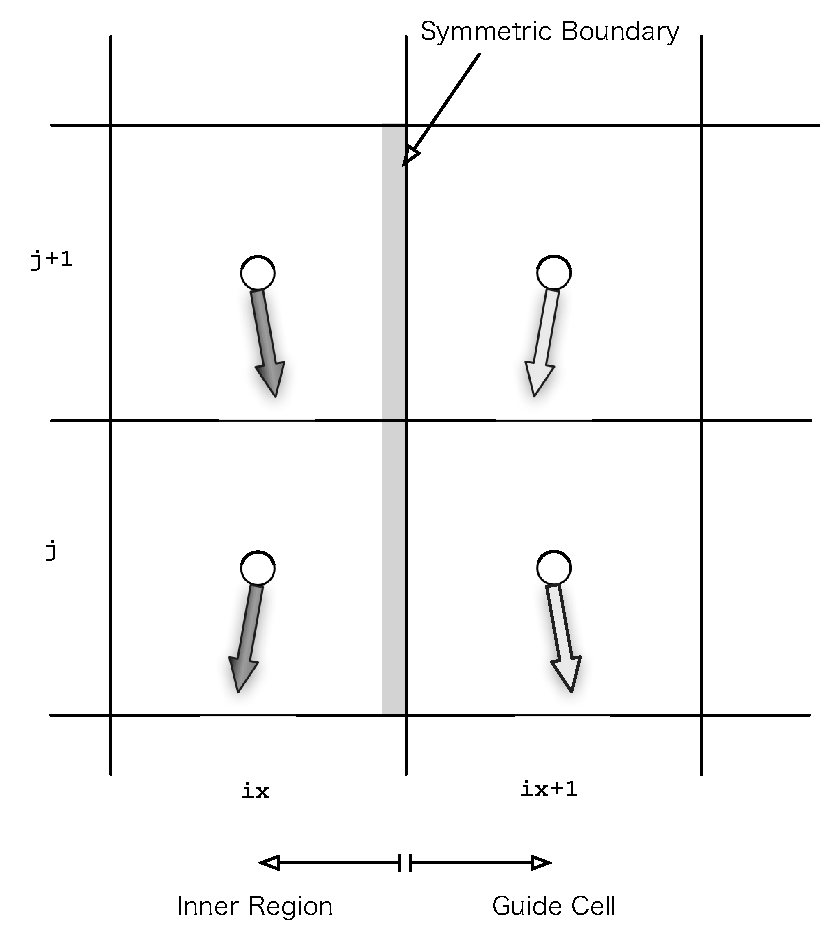
\includegraphics[width=7cm,clip]{symmetric.eps}
\end{center}
\caption{対称境界面における境界条件}
\label{fig:symmetric plane}
\end{figure}

熱計算では,対称境界が指定された面は断熱境界となります.


%%%
\pagebreak
\subsection{流出境界}

流出境界を指定する場合には,流出方向は既知とします.
外部境界では\textbf{図\ref{fig:outflow BC outer}}に示すようにガイドセルのセル属性は流体であることが必要です.
ガイドセルのセル属性の指定方法については\hyperlink{tgt:outer_boundary}{OuterBoundary}を参照してください.

{\small
\begin{program}
OuterBoundary {
  Basic_BCs[@] {
    alias    = "to_exhaust"
    class    = "outflow"
    velocity_type = "minmax"
  }
}
\end{program}
}

\begin{figure}[htbp]
\begin{center}
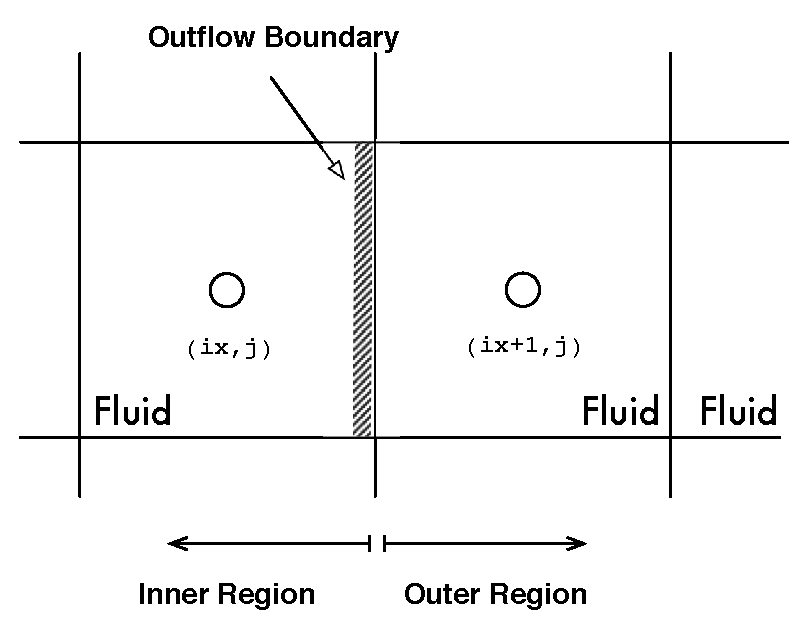
\includegraphics[width=8cm,clip]{outflowBC_outer.eps}
\end{center}
\caption{外部境界面における流出境界.x+方向の例.}
\label{fig:outflow BC outer}
\end{figure}

\noindent 指定するパラメータとして,対流流出速度の評価方法があります.この例では,流出速度の評価方法にMinmaxを指定しています.
流出速度の選び方として,流出断面の平均速度や最大値と最小値の算術平均などが提案されており,経験上,内部流の場合にはAverageが流出速度のよい近似値を与えます.
一方,外部流や噴流のような無限空間の境界面の場合にはMinMaxがよい近似値となります.
流出速度の指定は,\textbf{表\ref{tbl:outflow velocity}}のようにVelocity\_TypeタグにてAverage または Minmaxを指定します.
Averageは,物体でブロックされていない有効セルの平均値をとります.
Minmaxは,境界面における有効セルの流速の最大値と最小値の算術平均値を与えます.

\begin{table}[htdp]
\caption{対流流出速度の評価方法の指定}
\begin{center}
\small
\begin{tabular}{ll} \toprule
Velocity\_Type & パラメータの説明\\ \midrule
Average & 流出面の有効セルに対する平均値\\
Minmax & 流出面の有効セルに対する最大値と最小値の算術平均値\\ \bottomrule
\end{tabular}
\end{center}
\label{tbl:outflow velocity}
\end{table}

圧力境界条件としては,Fractional Step法のアルゴリズムに適合するように,境界面上で$\nabla p=0$を用いています.

熱境界としても,速度と同様に,対流流出型の境界条件となります.



%%
\pagebreak
\subsection{速度指定境界}

この境界条件は,セル界面における運動量流束の形で実装されています.
まず,速度指定境界のパラメータについて説明します.

{\small
\begin{program}
OuterBoundary {
  Basic_BCs[@] {
    alias    = "inlet"
    class    = "Specified_Velocity"
    Profile  = "Harmonic"
    Normal   = (0.0, 1.0, 0.0)
    amplitude= 7.0
    frequency= 2.0
    initial_phase = 0.0
    constant_bias = 0.0
    Temperature = 30.0
  }
}
\end{program}
}

\noindent 境界面の指定方法は,\textbf{表\ref{tbl:vspec parameter with heat}}に示すパラメータを与えます.
時間変化を伴う速度指定はProfile=\lq\lq Harmonic\rq\rq を指定し,\textbf{式(\ref{eq:harmonic out})}の形式の単振動の境界条件を周期や初期位相,固定バイアスと供に与えます.時間的に変化しない壁面境界の場合にはProfile=\lq\lq Constant\rq\rq を指定し,周波数,初期位相,固定バイアス値の指定は不要です.

圧力の境界条件は,壁面境界条件と同様にNeumann型の圧力境界条件$\nabla p=0$が用いられます.

温度の指定単位は,Unitセクションの\hyperlink{tgt:unit}{Temperature}で指定した単位になります.

\begin{table}[htdp]
\caption{速度指定境界のパラメータ}
\begin{center}
\small
\begin{tabular}{lll} \toprule
ラベル & 指定キーワード & パラメータの説明\\ \midrule
Normal & | & 法線ベクトルの成分\\
Velocity & | & 指定単位 $[m/s]$,Profile=constantの場合のみ\\
Amplitude & | & 速度,以下のパラメータはProfile=harmonicの場合のみ\\
Frequency & | & 周波数 $f\, [Hz]$\\
Initial\_Phase & | & 初期位相 $\phi\, [Rad]$\\
Constant\_Bias & | & 一定値 $b\, [m/s]$\\
Temperature & | & 指定温度 $[K\,|\,{}^\circ\mathrm{C}]$\\
\bottomrule
\end{tabular}
\end{center}
\label{tbl:vspec parameter with heat}
\end{table}


%%
\pagebreak
\subsection{周期境界}

\hypertarget{tgt:preriodic}{周期境界条件}には,外部境界に対する周期境界と計算内部領域に設定する部分的な周期境界条件を併用する条件の2種類があります.
外部境界に対する周期境界条件では,\textbf{図\ref{fig:index_domain}}において,Inner\,Regionの両端の境界が重なる状態を想定しています.

\vspace{2mm}

外部境界に対する周期境界条件には\textbf{表\ref{tbl:periodic mode}}に示す3つのモードが指定できます.
下記には,各モードの例を示します.
Simple\_Copyモードは,周期境界条件面の両端で,単純に計算内部領域の値を他方のガイドセルにコピーします.
Pressure\_Diffrenceモードは,両端で圧力差を与える周期境界条件で,速度や温度についてはSimple\_Copyモードと同じですが,圧力は指定の圧力差を与えます.上流側と下流側の設定が必要です.
Driverモードは,乱流計算などで発達したチャネル流を上流境界として与えるためのしくみで,局所境界条件との組み合わせで利用します.Driverモードの説明は局所境界条件をご覧ください.

{\small
\begin{program}
OuterBoundary {
  Basic_BCs[@] {
    alias    = "x-dir_periodic_1"
    class    = "periodic"
    Mode     = "Simple_Copy"
  }
  
  Basic_BCs[@] {
    alias    = "x-dir_periodic_2"
    class    = "periodic"
    Mode     = "Directional"
    flow_direction = "upstream"
    pressure_difference = 8.148e-3
  }
  
  Basic_BCs[@] {
    alias    = "x-dir_periodic_3"
    class    = "periodic"
    Mode     = "Directional"
    flow_direction = "downstream"
    pressure_difference = 8.148e-3
  }
  
  Basic_BCs[@] {
    alias    = "x-dir_periodic_3"
    class    = "periodic"
    Mode     = "driver"
    driver_direction = "x_minus"
  }
}
\end{program}
}

\begin{table}[htdp]
\caption{周期境界条件のモード}
\begin{center}
\small
\begin{tabular}{ll} \toprule
キーワード & モードの説明\\ \midrule
Simple\_Copy & 周期境界の両端で物理量をガイドセルにコピーします.\\
Directional  & 圧力差を与える周期境界条件で,上流と下流の境界面を指定します.\\
Driver       & 計算領域内で部分的な周期境界条件を設定します.\\ \bottomrule
\end{tabular}
\end{center}
\label{tbl:periodic mode}
\end{table}

Directionalモードでは,\textbf{表\ref{tbl:parameter dir. mode}}に示すパラメータが必要で,Pressure\_Differenceの値が,UpstreamとDownstreamで同じ値である必要があります.

\begin{table}[htdp]
\caption{Directionalモードに必要なパラメータ}
\begin{center}
\small
\begin{tabular}{ll} \toprule
必要なキーワード & パラメータの説明\\ \midrule
Pressure\_Difference & 両端にかける圧力差 $[Pa]$\\
Flow\_Direction & Upstream(上流面)または Downstream(下流面)\\
\bottomrule
\end{tabular}
\end{center}
\label{tbl:parameter dir. mode}
\end{table}



%%%
\pagebreak
\subsection{トラクションフリー境界}

遠方境界条件として,トラクションフリー条件を用います.

\vspace{2mm}

トラクションフリー条件は,外部境界に対してのみ指定できる境界条件で,計算対象の主領域から遠方の挙動を仮定した条件です.
つまり,圧力の遠方条件$p=0$(基準圧)を考慮し,計算外部境界において流体の内部応力の法線方向成分がゼロである仮定を用いています.
この境界条件は,噴流のエントレインメントの効果などを考慮できる利点がありますが,渦が流出するような境界には適用できません.

{\small
\begin{program}
OuterBoundary {
  Basic_BCs[@] {
    alias    = "ambient"
    class    = "Traction_Free"
    ambient_temperature = 25.0
  }
}
\end{program}
}

熱流れの場合には,遠方場における温度を指定します.



%%%
\pagebreak
\subsection{遠方境界}

外挿境界条件で,実験的な実装です.

\vspace{2mm}

指定された外部境界面において,外部境界面の値を内部から外挿して与えます.

{\small
\begin{program}
OuterBoundary {
  Basic_BCs[@] {
    alias    = "extrapolation"
    class    = "Far_Field"
    ambient_temperature = 25.0
  }
}
\end{program}
}

熱流れの場合には,流入時に対応する温度を指定します.



%%%-------------------------------------------------
\pagebreak
\section{局所境界条件}
内部領域の境界条件は,コンポーネントとして実装しています.
局所境界条件の多くは,計算空間内に局所的に存在し,複雑な計算処理を行います.
コンポーネントはそれらを効率よく取り扱うための機能です.
1つのセルを構成する6つの面にはそれぞれ別の境界条件を指定できますが,1つのセルには同種の流出境界は1種類だけしか設定できません.

%
\subsection{壁面境界}

\subsubsection{流れの境界条件}
計算領域内部の壁面境界条件は,モデルで固体壁に指定したセルが固体として認識され,セル界面の流束が指定する壁面速度から直接計算されるので,特に明示的な指定はありません.

壁面境界に対する圧力の境界条件は,Navier-Stokes方程式からNeumann型の圧力境界条件が得られます.
高レイノルズ数流れにおいては,粘性項の寄与が小さいと仮定し粘性項を省略し$\nabla p=0$の形式になります.
Binary近似の場合には,固体壁面との界面で$\nabla p=0$を満たすようにスキームが構成されています.

%
\subsubsection{熱境界条件}
壁面に対する熱境界条件としては,断熱,熱流束,熱伝達,等温,温度条件を指定できます.
熱境界条件の実装の詳細はInside\_FFVC.pdfをご覧ください.

%
\paragraph{熱境界条件の指定方法}
\hypertarget{tgt:spec of heat bc}{熱境界条件}は,セルの界面に与えます.多くの場合は流体と固体の界面ですが,固体熱伝導と共役熱移動の場合には,固体-固体界面の場合もあります.
局所境界の場合の界面の指定方法としては,指定する2つのIDで挟まれるボクセルの構成面を指定界面とします.
指定するIDの一つはキーIDで,主に固体セルを指定します.もうひとつのIDはDef\_Face IDです.

熱境界条件をコンポーネントとして与える場合,固体面をキーIDに指定します.
このときの熱流束の方向は,
\textbf{図\ref{fig:heat bc on solid}}において,固体面から流体側へ向かう法線をと同じ方向です.
つまり,この法線方向が指定する値の正の方向とし,流体側への熱移動を正の方向と考えます.

\begin{figure}[htbp]
\begin{center}
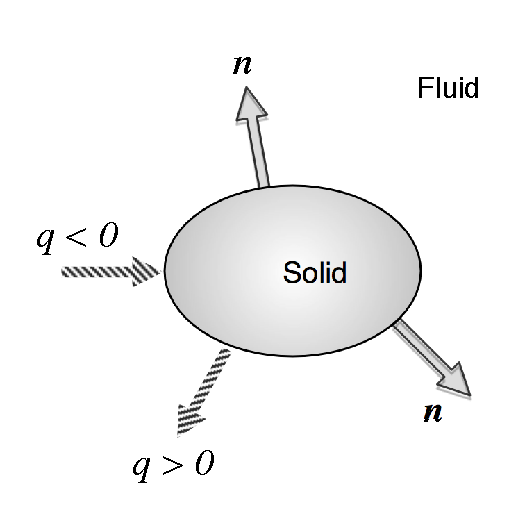
\includegraphics[width=6cm,clip]{heatBC.eps}
\end{center}
\caption{流体-固体界面における熱境界条件の熱流束の方向}
\label{fig:heat bc on solid}
\end{figure}

CBCの熱流体解析には幾つかのモードがあります.\hyperlink{tgt:solver_property}{Kind\_of\_Solver}の指定モードによって,計算空間内の計算対象とする部分が異なります.
Thermal\_FlowとThermal\_Flow\_Naturalの場合は,熱流動計算で流体の温度のみを解きます\footnote{計算の実装上,固体部分も解いていますが,その値はマスクされ,無効化されています.}.したがって,固体部分は計算対象とはならず不活性セルとして扱います.これより,流体-固体の境界面で与える熱境界条件(熱流束)は,流体セル側のみに指定されます.

一方,Solid\_Conductionの場合は,固体部分の熱伝導のみを解くので,流体部分を不活性セルとして扱います.したがって,流体-固体の境界面で与える熱境界条件は,固体セル側のみに指定されます.

Conjugate\_Heat\_Transferの場合には,流体と固体の両方の熱移動を計算します.したがって,流体-固体の境界面で与える熱境界条件は,流体セルと固体セルの両方で指定されます.

以下の各境界条件の指定で述べるように,IDとDef\_Faceタグの組み合わせにより,流体-固体の境界面を指定します.
このとき,\textbf{IDには固体のIDを,Def\_Faceには流体または固体のIDを指定すること}を基本としてください\footnote{IDに固体を指定する理由は,参照範囲を小さく抑えて効率的な計算をするためです.}.

%
\paragraph{断熱境界}
断熱壁では指定面で熱流束がゼロ,つまり$q^{\prime}=0$を指定します.固体セルと流体セルの界面に何も熱境界条件を指定しなければ,断熱境界条件となります.また,明示的に次のように\lq\lq Adiabatic\rq\rq セクションで断熱面を指定することができます.

{\small
\begin{program}
<LocalBoundary>
  <Elem name="Adiabatic" ID="6" comment="shield">
    <Param name="Def_Face" dtype="INT" value="3"/>
  </Elem>
</LocalBoundary>
\end{program}
}
この例では,ID=\lq\lq 6\rq\rq の固体セルのうち,ID=\lq\lq 3\rq\rq の流体セルに接する面に対して,断熱境界条件を指定しています.

%
\paragraph{熱流束境界}
熱流束境界は境界面で指定の熱流束を与えます.

{\small
\begin{program}
<LocalBoundary>
  <Elem name="Direct_Heat_Flux" ID="6" comment="outer_wall">
    <Param name="Def_Face"    dtype="INT"    value="3"/>
    <Param name="Heat_Flux"   dtype="REAL"   value="10.0"/>
  </Elem>
</LocalBoundary>
\end{program}
}

%
\paragraph{熱伝達境界}
熱伝達境界は次式の形式で熱流束を与える条件で,幾つかの種類があります.固体-流体セル間の熱伝達境界の与え方は,\hyperlink{tgt:heat-transfer}{外部境界条件の熱伝達境界}で説明した内容と同じです.

\begin{indentation}{3zw}{0zw}
%
\subparagraph{Type\_S  表面温度と熱伝達係数により計算}
Type\_Sは固体表面温度と熱伝達係数を与え,熱流束を計算します.
\textbf{式(\ref{eq:ht form})}において,$\theta_{\infty}^{\prime}$を固体表面に接する流体セルの値と仮定します.
以下に,熱境界部分のみパラメータ指定の一例を示します.

{\small
\begin{program}
<LocalBoundary>
  <Elem name="HeatTransfer_S" ID="6" comment="engine">
    <Param name="Def_Face"              dtype="INT"  value="3"/>
    <Param name="Surface_Temperature"   dtype="REAL" value="300.0"/>
    <Param name="Coef_of_Heat_Transfer" dtype="REAL" value="20.0"/>
  </Elem>
</LocalBoundary>
\end{program}
}

%
\subparagraph{Type\_SN  自然対流の乱流熱伝達}
自然対流の場合の乱流熱伝達の実験式を実装した境界条件です.

{\small
\begin{program}
<LocalBoundary>
  <Elem name="HeatTransfer_SN" ID="6" comment="engine">
    <Param name="Def_Face"                 dtype="INT"    value="3"/>
    <Param name="Surface_Temperature"      dtype="REAL"   value="500.0"/>
    <Param name="Ref_Temp_Mode"            dtype="STRING" value="Bulk_Temperature"/>
    <Param name="vertical_laminar_alpha"   dtype="REAL"   value="0.59"/>
    <Param name="vertical_laminar_beta"    dtype="REAL"   value="0.25"/>
    <Param name="vertical_turbulent_alpha" dtype="REAL"   value="0.1"/>
    <Param name="vertical_turbulent_beta"  dtype="REAL"   value="0.3333333"/>
    <Param name="vertical_ra_critial"      dtype="REAL"   value="1.0e9"/>
    <Param name="lower_laminar_alpha"      dtype="REAL"   value="0.27"/>
    <Param name="lower_laminar_beta"       dtype="REAL"   value="0.25"/>
    <Param name="lower_turbulent_alpha"    dtype="REAL"   value="0.27"/>
    <Param name="lower_turbulent_beta"     dtype="REAL"   value="0.25"/>
    <Param name="lower_ra_critial"         dtype="REAL"   value="1.0e9"/>
  </Elem>
</LocalBoundary>
\end{program}
}

%
\subparagraph{Type\_SF  強制対流の層流・乱流熱伝達}
強制対流の場合の層流・乱流熱伝達の実験式を実装した境界条件です.

{\small
\begin{program}
<LocalBoundary>
  <Elem name="HeatTransfer_SF" ID="6" comment="engine">
    <Param name="Def_Face"            dtype="INT"    value="3"/>
    <Param name="Surface_Temperature" dtype="REAL"   value="500.0"/>
    <Param name="Ref_Temp_Mode"       dtype="STRING" value="Bulk_Temperature"/>
    <Param name="alpha"               dtype="REAL"   value="0.037"/>
    <Param name="beta"                dtype="REAL"   value="0.8"/>
    <Param name="gamma"               dtype="REAL"   value="0.333333"/>
  </Elem>
</LocalBoundary>
\end{program}
}

%
\subparagraph{Type\_B  固体壁からの放熱条件}
熱伝達係数とバルク温度を与え,熱流束を計算します.固体熱伝導を解く場合の境界条件として利用します.

{\small
\begin{program}
<LocalBoundary>
  <Elem name="HeatTransfer_B" ID="6" comment="engine">
    <Param name="Def_Face"              dtype="INT"    value="3"/>
    <Param name="Bulk_Temperature"      dtype="REAL"   value="500.0"/>
    <Param name="Coef_of_Heat_Transfer" dtype="REAL"   value="0.12"/>
  </Elem>
</LocalBoundary>
\end{program}
}

\end{indentation}


%
\paragraph{等温壁境界}
等温壁境界は,指定面で温度が一定となる境界条件で,面温度を一定に保つような熱流束が発生します.

{\small
\begin{program}
<LocalBoundary>
  <Elem name="IsoThermal" ID="6" comment="outer_wall">
    <Param name="Def_Face"    dtype="INT"    value="3"/>
    <Param name="Temperature" dtype="REAL"   value="100.0"/>
  </Elem>
</LocalBoundary>
\end{program}
}


%%
\subsection{流出境界条件}

\paragraph{流れの境界条件}
計算領域内部に設定する流出境界について説明します.
\textbf{局所境界の場合には流出側のセルは固体セルであり,かつ流出方向に2セル必要になること}に注意してください.
つまり,\textbf{図\ref{fig:outflow BC inner}}においては,セル$(i,\,j)$は流体,セル$(i+1,\,j)$は固体を指定します.
ハッチング部分,つまり$(i,\,j)$セルの固体セルに隣接する面が流出境界として指定されています.
計算内部領域における境界面は,次のように対象となる面をid=20とid=210の2つのIDで挟むことにより指定します.
速度の流出面における対流速度の評価方法として流出コンポーネントの平均速度を用い,流出面における圧力境界は圧力勾配ゼロとしています.

{\small
\begin{program}
<LocalBoundary> 
  <Elem name="outflow" id="20" comment="out">
    <Param name="def_face"    dtype="INT"    value="210" />
  </Elem>
</LocalBoundary>
\end{program}
}

\begin{figure}[htbp]
\begin{center}
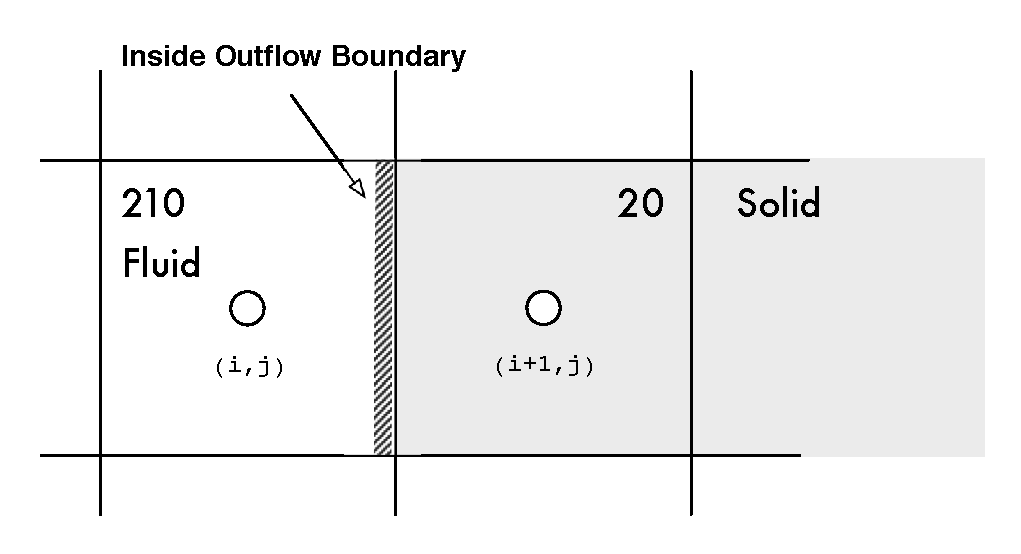
\includegraphics[width=8cm,clip]{outflowBC_inner.eps}
\end{center}
\caption{計算内部領域における流出境界の設定}
\label{fig:outflow BC inner}
\end{figure}

%
\paragraph{熱流出境界}
熱の流出境界は,流出界面の対流熱流束$\tilde{f}$を一次風上の形式で評価します.

\begin{equation}
\tilde{f} \,=\, \frac{\partial}{\partial x^{\prime}}\, \left( u^{\prime}\,\theta^{\prime} \right)_{upstream\_face}
\label{eq:outflow heat flux}
\end{equation}

分離解法において温度輸送方程式を解く過程では,速度は既知なので上式は直ちに計算できます.


%%%
\subsection{速度指定条件}

\paragraph{流れの境界条件}
この境界条件は,セル界面の運動量流束の形で実装されています.
まず,計算内部領域における流入境界の入力パラメータについて説明します.

{\small
\begin{program}
LocalBoundary {
  alias = "inlet"
  class = "specified_velocity"
  normal= (0.0, 0.0, -1.0)
  type  = "velocity"
  profile = "constant"
  velocity= 3.0
  temperature = 60.0
  BC_Direction = "opposite"
}
\end{program}
}

\noindent 境界面の指定方法は\textbf{表\ref{tbl:spec_vel}}に示すパラメータを与えます.
時間変化を伴う速度指定はProfile=\lq\lq Harmonic\rq\rq を指定し,\textbf{式(\ref{eq:harmonic_inner})}の形式の単振動\index{たんしんどう@単振動}の境界条件を周期や初期位相,固定バイアスと供に与えます.時間的に変化しない壁面境界の場合にはProfile=\lq\lq Constant\rq\rq を指定し,周波数,初期位相,固定バイアス値の指定は不要です.

\begin{equation}
V \,{=}\, A \sin \left( 2 \mathrm{\pi} ft \,+\, \phi \right) \,+\, b
\label{eq:harmonic_inner}
\end{equation}

\begin{table}[htdp]
\caption{コンポーネントの流束指定のパラメータ}
\begin{center}
\small
\begin{tabular}{ll} \toprule
ラベル & パラメータの説明\\ \midrule
Normal & 法線ベクトルの成分\\
Type & 指定速度のモード (Velocity $|$ Massflow)\\
Profile & 指定速度のタイプ (Constant $|$ Harmonic)\\
Velocity & 速度$[m/s]$ または 流量$[m^3/sec.]$,Profile=constantの場合のみ\\
Amplitude & 速度,流量,以下のパラメータはProfile=harmonicの場合のみ\\
Frequency & 周波数 $f\, [Hz]$\\
Initial\_Phase & 初期位相 $\phi\, [Rad]$\\
Constant\_Bias & 一定値 $b\, [m/s]$ または $[m^3/sec.]$\\
Temperature & 熱計算の場合に流入温度$[K\,|\,{}^\circ\mathrm{C}]$を指定\\
\bottomrule
\end{tabular}
\end{center}
\label{tbl:spec_vel}
\end{table}

\paragraph{熱境界条件}
指定面での対流熱流束を\textbf{式(\ref{eq:outflow heat flux})}で評価します.


%%%
\subsection{周期境界条件}
内部周期境界条件は外部の周期境界条件と組み合わせて利用します.
このため,外部境界条件指定で,次の指定が必要です.

{\small
\begin{program}
<OuterBoundary>
  <Elem name="Basic_BCs">
    <Elem name="periodic" id="10" >
      <Param name="mode"             dtype="string" value="driver" />
      <Param name="driver_direction" dtype="string" value="x_minus" />
    </Elem>
  </Elem>
</OuterBoundary>
\end{program}
}

\begin{table}[htdp]
\caption{Driverモードのパラメータ}
\begin{center}
\small
\begin{tabular}{ll} \toprule
必要なキーワード \\ \midrule
Driver\_Direction & X\_minus$\,|\,$X\_plus$\,|\,$Y\_minus$\,|\,$Y\_plus$\,|\,$Z\_minus$\,|\,$Z\_plus\\ \bottomrule
\end{tabular}
\end{center}
\label{tbl:parameter driver mode}
\end{table}

\paragraph{流れの境界条件}
内部の周期境界条件は,計算外部と計算領域内で部分的な周期境界条件を設定します.
モードとしてDriverを指定した場合には,下記のように同時に内部周期境界を指定しなければなりません.
Upstream\_DirectionとOuterBoundaryで指定するDriver\_Directionの方向は一致する必要があります.

{\small
\begin{program}
<LocalBoundary>
  <Elem name="periodic" id="4" comment="inner_driver" >
    <Param name="upstream_direction"  dtype="string" value="x_minus" />
    <Param name="pressure_difference" dtype="REAL"   value="1.636e-4" />
  </Elem>
</LocalBoundary>
\end{program}
}

現時点では,逐次計算しかできません.

\paragraph{熱境界条件}
熱境界に対しては,指定するパラメータはありません.


%%%
\subsection{セルボリュームに対する熱境界条件}
セル体積要素に作用するコンポーネントの熱境界条件を説明します.
この境界条件は,全てのセルに対して適用可能です.

\subsubsection{Specified\_Temperature}

以下の形式で指定温度を与えます.
{\small
\begin{program}
<LocalBoundary>
  <Elem name="Specified_Temperature" ID="60" comment="engine">
    <Param name="Temperature" dtype="REAL" value="45.0"/>
  </Elem>
</LocalBoundary>
\end{program}
}

\begin{table}[htdp]
\caption{温度指定のパラメータ}
\begin{center}
\small
\begin{tabular}{ll} \toprule
指定キーワード & パラメータの説明\\ \midrule
Temperature & 表面温度 $[K\,|\,{}^\circ\mathrm{C}]$\\
\bottomrule
\end{tabular}
\end{center}
\label{tbl:spec temp}
\end{table}

%
\subsubsection{Heat\_Generation}
\textbf{表\ref{tbl:heat_generation}}に示すように,発熱量または発熱密度を指定セルに与えることができます.
発熱量を指定した場合には,該当IDの体積を前処理で計算し,発熱密度に変換します.
次の例では,ID=60に10[$W$]の発熱量を与えています.

{\small
\begin{program}
<LocalBoundary>
  <Elem name="Heat_Source" ID="60" comment="heater">
    <Param name="Type"    dtype="STRING" value="Heat_Release_Value"/>
    <Param name="Value"   dtype="REAL"   value="10.0"/>
  </Elem>
</LocalBoundary>
\end{program}
}

\begin{table}[htdp]
\caption{発熱セルの指定方法}
\begin{center}
\small
\begin{tabular}{lll} \toprule
キーワード & パラメータの種類 & 単位\\ \midrule
Heat\_Release\_Value & 発熱量 & $[W]$\\
Heat\_Generation\_Density & 発熱密度 & $[W/m^3]$\\ \bottomrule
\end{tabular}
\end{center}
\label{tbl:heat_generation}
\end{table}


%%%
\subsection{不活性セル指定}

計算空間内で,\hypertarget{tgt:inactive}{不活性化するセル}を指定します.
コンポーネントの機能を使って実装しています.
\vspace{2mm}

不活性化の対象は,圧力と温度の計算に対してのみで,流体と固体の両方の属性をもつセルIDに適用できます.
不活性を指定されたセルは,圧力と温度の計算に関しては,意味のある計算をしません.代わりに,周囲のセルの平均値が代入されます.この処理はラプラス方程式を解くことに相当しますが,収束判定時にはその残差は考慮しません.下記のように,不活性化するセルIDを指定します.

{\small
\begin{program}
<LocalBoundary>
  <Elem name="Inactive" ID="600" comment="outer_layer"/>
</LocalBoundary>
\end{program}
}


%%%
\subsection{モニタ}
\hypertarget{tgt:localBCmonitor}{局所境界条件}のしくみを用いたサンプリング設定について説明します.
計算空間内に設定する局所境界条件について,コンポーネント毎の積算値をモニターします.
下記の例では,ID=20で指定される領域をモニタ部とし,そこで速度,圧力をモニタすることを指定しています.
Normalはモニタ面の法線を指定しています.

{\small
\begin{program}
<LocalBoundary>
  <Elem name="Cell_Monitor" id="20" comment="monitor_inlet"> 
    <Param name="Normal_x" dtype="REAL" value="1.0" /> 
    <Param name="Normal_y" dtype="REAL" value="0.0" /> 
    <Param name="Normal_z" dtype="REAL" value="0.0" /> 
    <Elem name="Variables"> 
      <Param name="velocity"       dtype="STRING" value="on" /> 
      <Param name="pressure"       dtype="STRING" value="on" /> 
      <Param name="temperature"    dtype="STRING" value="off" /> 
      <Param name="Total_pressure" dtype="STRING" value="off" /> 
    </Elem> 
  </Elem>
</LocalBoundary>
\end{program}
}

指定方法の詳細は,\hyperlink{tgt:cell_monitor}{ボクセルモデルのセルIDで指定する方法}を参照してください.


%%
\hypertarget{tgt:external forcce}{\section{外力項を用いた境界条件}}

流動現象の中には空間スケールの異なる流れがあり相互に影響するような問題,例えば,多孔質層を通過する大空間の流れを解析する場合,興味の対象は大空間内の流動挙動であり,多孔質層内はマクロに見て適切な流れ場になっていればよいことも多くあります.
メッシュ解像度以下の微細な構造が流動特性に与える影響は,ダルシー則などのように理論的,あるいは実験式などで与えられます.
このような流体特性をもつ境界条件について説明します.

\subsection{圧力損失境界条件}
熱交換器やファンなどの圧力損失\index{あつりょくそんしつ@圧力損失}・利得をモデル化した境界条件について説明します.
熱交換器は,圧力損失を生じる多孔質物体として扱い,流出方向を法線で指定します.
この条件は,通過流量(流速)と圧力損失量の関係式が与えられるものとします.

一方,ファンは圧力利得が関係式として与えられます.
ファンの場合には旋回成分などもありますが,ここでは軸流方向のみを考えます.
このような流体部品のモデル指定は,セルボリュームに作用する局所境界条件として指定します.
具体的には,コンポーネント\index{コンポーネント}のPressure\_Lossとして扱い,\textbf{式(\ref{eq:ploss_NS})}の外力項$F_{i}$として実装します.
$\beta$はセル内部におけるコンポーネントの体積占有率\index{せんゆうりつ@占有率}(Volume Fraction; VF)\index{Volume Fraction}です.
外力項として,\textbf{表\ref{tbl:ploss_model}}のようなモデルが実装されています.

この境界条件に対応するモニタ量として,指定部の平均速度・流量や圧力損失量がhistory\_compo.logに書き出されます.
詳細は\hyperlink{tgt:history_compo}{コンポーネント履歴}を参照してください.

\begin{table}[htdp]
\caption{セルボリュームに作用する局所境界条件}
\begin{center}
\small
\begin{tabular}{ll} \toprule
キーワード & 境界条件モデル \\ \midrule
%Fan & ファンモデル  \\ 
Pressure\_Loss & 熱交換器モデル \\ 
%Darcy & 多孔質体に対するDarcyモデル & \\ 
\bottomrule
\end{tabular}
\end{center}
\label{tbl:ploss_model}
\end{table}

\begin{equation}
{\frac{\partial{u}_{i}}{\partial{t}}}^{{n}{+}{1}}{+}\,\frac{\partial}{\partial{x}_{j}}\left({{u}_{i}{u}_{j}}\right)
\,{=}\,
{-}{\frac{\partial{p}}{\partial{x}_{i}}}^{{n}{+}{1}}{+}\,{(}{1}{-}\mathrm{\beta}{)}\frac{\partial{\mathrm{\tau}}_{ij}}{\partial{x}_{j}}\,{+}\,\beta {F_{i}}^{n+1}
\label{eq:ploss_NS}
\end{equation}

%
\paragraph{熱交換器のモデル化}

圧力損失の一つである熱交換器モデルは,\textbf{式(\ref{eq:ploss_NS})}に\textbf{式(\ref{eq:ploss_force})}の実験式を適用します.
\begin{equation}
{F}_{i}
\,{=}\,
-sgn \left( u_{i} \right) {\left( \frac{\Delta p}{\Delta r} \right)}^{R} {n_{i}}^{R}
\label{eq:ploss_force}
\end{equation}

\noindent ここで,${}^{R}$は熱交換器を表し,$\Delta p,\,\Delta r,\,n_{i}$はそれぞれ圧力損失量,熱交換器の厚さ,法線方向を表します.
熱交換機の通過ベクトルとは逆方向に圧力損失が発生するモデルとなっています.
ただし,パラメータvectorがdirectionalでない場合には,速度ベクトルは熱交換器の流出方向には揃わず.単に,圧力損失が計算された速度ベクトルと逆向きに作用するモデルとなります.
圧力損失パラメータは,熱交換器の性能試験結果により,\textbf{図\ref{fig:ploss}}に示すような実験値が得られます.
$\Delta p-V$の性能線図を$[mmAq - m/s]$を単位とした場合のパラメータの取得について示します.
熱交換器の圧力損失は,二次多項式で近似できます.
\textbf{図\ref{fig:ploss}}のグラフの読みからカーブフィットを行い,\textbf{式(\ref{eq:dp-v})}に対応する数値$c_{1}$ -- $c_{4}$, $u_{threshold}$を得ます.ダッシュは有次元を表します.
このとき,圧力損失ヘッドの単位に応じて,パラメータは無次元量に変換されます.
\begin{equation}
{h}^{\prime}
\,{=}\,
\begin{cases}
\, c_{1} {u^{\prime}}^{2}\,+\,c_{2}u^{\prime}\,+\,c_{3} & \quad (u^{\prime} \geqq u^{\prime}_{threshold})\\
\, c_{4} {u^{\prime}}^{2} & \quad (u^{\prime}<u^{\prime}_{threshold})\\
\end{cases} \quad [mm]
\label{eq:dp-v}
\end{equation}

\begin{figure}[htdp]
\begin{center}
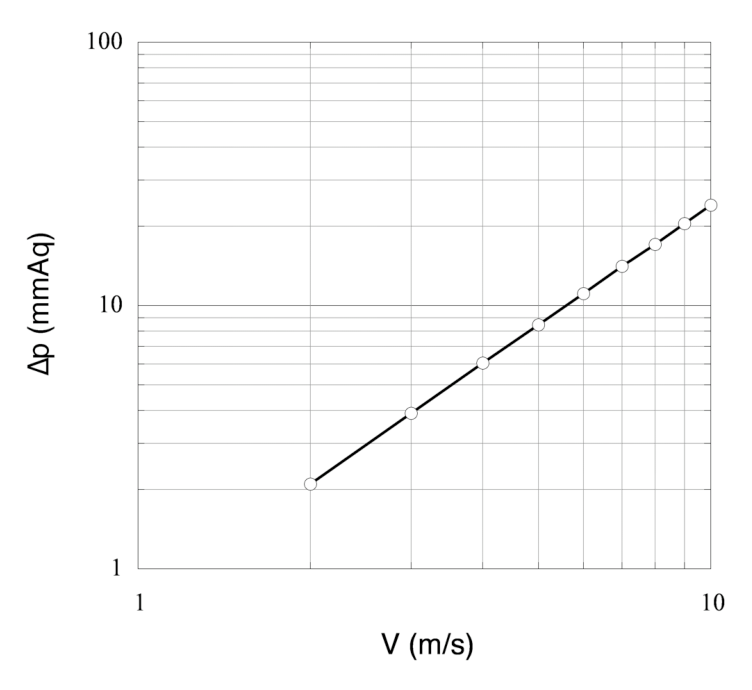
\includegraphics[width=10cm,clip]{ploss.eps}
\end{center}
\caption{$\Delta p-V$性能線図(対数表示)}
\label{fig:ploss}
\end{figure}

\begin{figure}[htdp]
\begin{center}
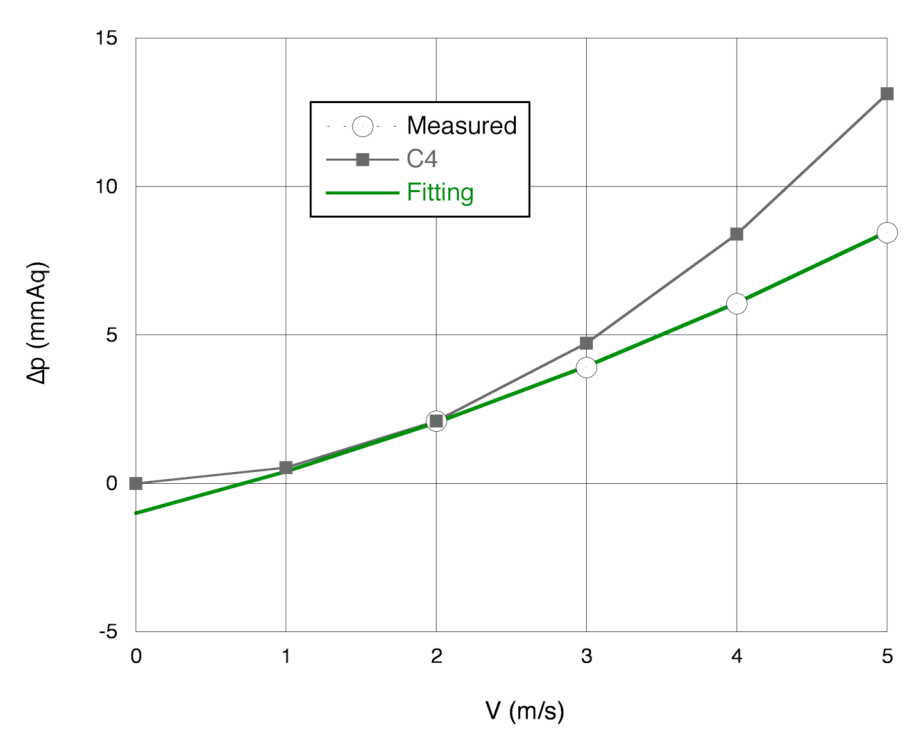
\includegraphics[width=10cm,clip]{rad_para.eps}
\caption{パラメータの取得(\textbf{図\ref{fig:ploss}}と同じものを線形表示)}
\label{fig:get_para}
\end{center}
\end{figure}

\textbf{図\ref{fig:get_para}}に計算パラメータの取得方法を示します.一般に,低速域のデータは得られない場合が多く,推定が必要です.
図では○が測定結果を示し2$[m/s]$より低速域のデータはありません.
そこで,測定値を元にカーブフィッティングを行い(図中の緑色の曲線),算出された係数$c_{1}=0.12321,\,c_{2}=1.2806,\,c_{3}=-1.0074\quad(2-10\,[m/s])$を計算パラメータとします.
この場合,$h'$切片がマイナスになるため,熱交換機の通過速度がゼロに近い場合に急にマイナスの圧力損失(つまり圧力利得)が発生し,実際の現象とは異なり計算上好ましくありません.
そこで\textbf{式(\ref{eq:dp-v})}に示すようにある閾値で曲線を切り替えます.
ここでは,測定された最小速度$u_{threshold}=2\,[m/s]$を閾値として,C4のカーブ$c_{4}=0.525\quad(0-2\,[m/s])$で切り替えます.
熱交換器厚さは実務での観点から単位を$[mm]$で指定するので,注意してください.\\

次の例では,境界条件番号8に圧力損失条件を設定します.
ここで各パラメータは\textbf{表\ref{tbl:ploss_table_ibc}}に対応します.

{\small
\begin{program}
<LocalBoundary>
  <Elem name="Pressure_Loss" ID="8" comment="radiator"/>
    <Param name="Unit"        dtype="STRING" value="mmAq"/>
    <Param name="Normal_x"    dtype="REAL"   value="1.0" />
    <Param name="Normal_y"    dtype="REAL"   value="0.0" />
    <Param name="Normal_z"    dtype="REAL"   value="0.0" />
    <Param name="c1"          dtype="REAL"   value="0.8" />
    <Param name="c2"          dtype="REAL"   value="0.0" />
    <Param name="c3"          dtype="REAL"   value="0.0" />
    <Param name="c4"          dtype="REAL"   value="0.8" />
    <Param name="u_threshold" dtype="REAL"   value="0.2" />
    <Param name="Thickness"   dtype="REAL"   value="80" />
    <Param name="Vector"      dtype="STRING" value="Directional" />
  </Elem>
</LocalBoundary>
\end{program}
}

\begin{table}[htdp]
\caption{圧力損失モデルのパラメータ}
\begin{center}
\small
\begin{tabular}{lll} \toprule
キーワード & パラメータの説明\\ \midrule
Normal\_x & 熱交換器の法線ベクトルのx方向成分\quad 法線は単位ベクトル\\
Normal\_y & 熱交換器の法線ベクトルのy方向成分\quad 法線は単位ベクトル\\
Normal\_z & 熱交換器の法線ベクトルのz方向成分\quad 法線は単位ベクトル\\
c1 & 熱交換器の圧力損失係数\,c1\quad $[mmAq\,|\,mmHg\,|\,Pa\,|\,Non dimension]$\\
c2 & 熱交換器の圧力損失係数\,c2\quad $[mmAq\,|\,mmHg\,|\,Pa\,|\,Non dimension]$\\
c3 & 熱交換器の圧力損失係数\,c3\quad $[mmAq\,|\,mmHg\,|\,Pa\,|\,Non dimension]$\\
c4 & 熱交換器の圧力損失係数\,c4\quad $[mmAq\,|\,mmHg\,|\,Pa\,|\,Non dimension]$\\
u\_threshold & 圧力損失カーブの切り替え速度 $u_{threshold}$ $[m/s\,|\,Non dimension]$\\
thickness & 熱交換器の厚さ\quad $[mm\,|\,Non dimension]$\\
unit & 圧力損失$\Delta p-V$線図のヘッドの単位\quad [$mmAq\,|\,mmHg\,|\,Pa\,|\,Non-Dimension]$ \footnotemark[4]\\
vector & 速度ベクトルの法線方向への強制\quad $[Directional \,|\, Non\_Directional]$\\  \bottomrule
\end{tabular}
\end{center}
\label{tbl:ploss_table_ibc}
\end{table}
\footnotetext[4]{mmAqは水(300K, p=101.325kPa)996.62 $[kg/m^3]$,mmHgは水銀(300K)13538 $[kg/m^3]$をプログラム中でハードコード.}


%%%
\begin{comment}

%
\paragraph{Fan}
\begin{indentation}{3zw}{0zw}
Fanモデル...
\end{indentation}

%
\paragraph{Darcy model}
\label{Darcy model param}
\begin{indentation}{3zw}{0zw}

\ref{sec:porous model}で説明したDarcyモデルでは,等方と非等方モデルが利用できる.透過率パラメータは,\textbf{表\ref{tbl:permeability parameter}}に示すように各主軸方向毎に与える.等方モデルの場合には,各方向のパラメータを同じ値にする.

{ \small
\begin{program}
<Elem name="Forcing_Volume" id="1">
  <Elem name="Darcy" id="50" comment="porous">
    <Param name="permeability_x"  dtype="REAL" value="2.0" />
    <Param name="permeability_y"  dtype="REAL" value="3.0" />
    <Param name="permeability_z"  dtype="REAL" value="4.0" />
  <\Elem>
<\Elem>
\end{program}
}

\begin{table}[htdp]
\caption{Darcyモデルのパラメータ}
\begin{center}
\small
\begin{tabular}{ll} \toprule
キーワード & パラメータの説明\\ \midrule
permeability\_x & x方向の透過率 $[m^2]$\\
permeability\_y & y方向の透過率 $[m^2]$\\
permeability\_z & z方向の透過率 $[m^2]$\\ \bottomrule
\end{tabular}
\end{center}
\label{tbl:permeability parameter}
\end{table}

\end{indentation}

\end{comment}
%%%




%%%
\section{静止座標系と移動座標系の場合の境界条件}
\label{sec:moving_grid}

外部流を考えます.
\textbf{図\ref{fig:reference_frame}}(a)の静止座標系\index{ざひょうけい@座標系!せいし@静止---}と\textbf{図\ref{fig:reference_frame}}(b)の移動座標系\index{ざひょうけい@座標系!いどう@移動---}のように異なる座標系で物体まわりの流れを計算する場合,境界条件の与え方が異なります.
静止座標系は風洞実験に相当し,静止した対象物に対して風をあてている状況です.テストセクション(この場合は計算領域)から出ていく流れが流出風に相当します.
一方,移動座標系では対象物に固定した計算格子が対象物とともに静止流体中を移動します.この場合は,計算領域そのものと内部の格子が物体とともに動きます.
一定速度$V$で動いている座標系の添え字を${}_M$とし,静止した座標系の添え字を${}_S$とします.
いま,静止座標系で観測される流体の速度を$u_{S}$と表すと,同じ速度は移動座標系では$u_{M}-V$のように観測されます.
つまり,
\begin{equation}
u_{S} \, = \, u_{M}-V
\label{eq:galilei}
\end{equation}

\begin{figure}[htbp]
\begin{center}
\subfigure[静止座標系]{
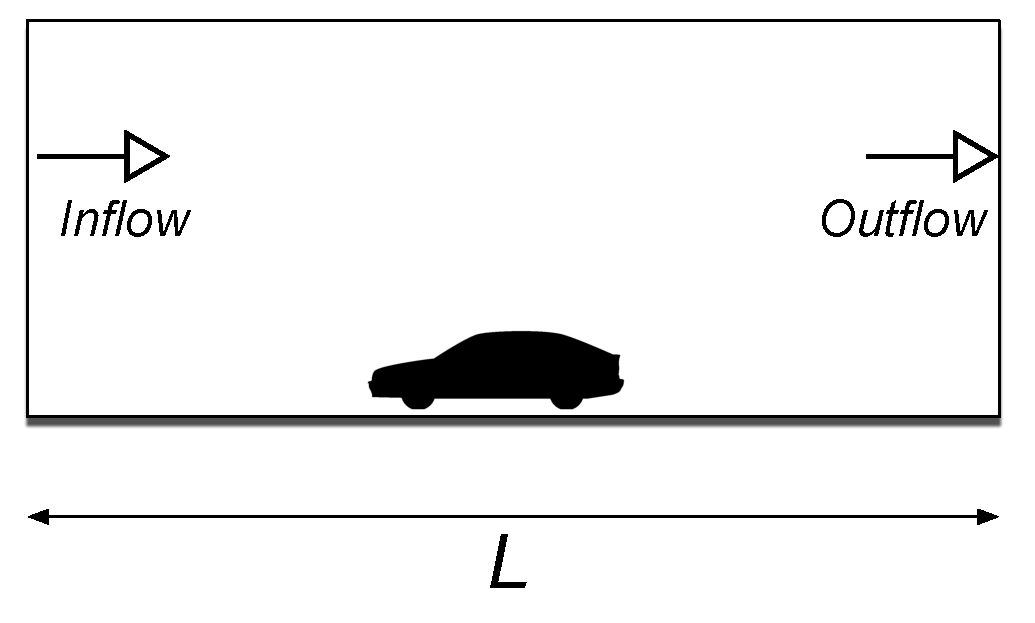
\includegraphics[width=8cm,clip]{stationary.eps}
}
~
\subfigure[移動座標系]{
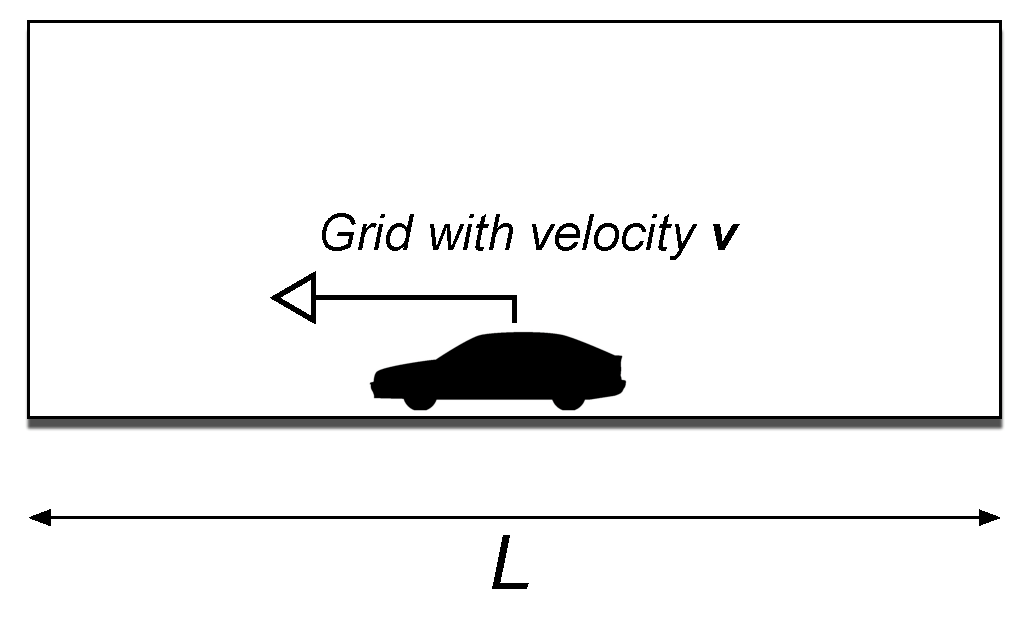
\includegraphics[width=8cm,clip]{moving.eps}
}
\caption{静止座標系と移動座標系の観測点の違い} 
\label{fig:reference_frame}
\end{center}
\end{figure}

静止座標系において\textbf{図\ref{fig:reference_frame}}(a)のような境界条件を与える場合,流入部では$u_{0}$を与えます.
一方,移動座標系では静止流体の条件,つまり$u=0,\,p=0$を想定し,格子速度$V=-u_{0}$を与えると両者は等価になります.

移動座標系の場合注意を要するのが,物体と地面の境界条件です.物体は移動しているので格子速度と同じになります.
一方,地面は静止している地面と動いている地面の二通りが考えられます.
前者は風洞実験で固定地面板に相当し,後者はムービングベルトに相当します.
ムービングベルトの場合には物体と格子速度だけ相対速度をもっていることになります.
したがって,

\begin{equation}
u_{ground}\,=\,
\begin{cases}
\, -u_{0} & \quad (Stationary\,ground)\\
\, 0 & \quad (Moving\,ground)\\
\end{cases}
\label{eq:relative velocity wall}
\end{equation}

移動格子の移動速度は\hyperlink{tgt:reference_frame}{Reference\_Frame}セクションで与えます.






%



%%%
\chapter{モニタリング機能}
\label{chpt:monitor}

\begin{abstract}
FFV-Cソルバーには,計算中の任意点の物理量をモニターする仕組みがあります.本章では,その指定方法について説明します.
\end{abstract}
%
\graphicspath{{./fig_Monitor/}}


物理量モニタリング機能は,ユーザが指定した位置で指定した物理量をファイルに出力する機能です.
位置の指定には,パラメータファイルで指定する方法と解析モデルのラベルで指定する方法の2種類があります.


%%%
\section{パラメータファイルで指定する方法}
モニタリングの指定は,Monitor\_Listセクションに記述します.

{\small
\begin{program}
<Elem name="Monitor_List"> 
  <Param name="Log"                    dtype="STRING" value="On" />
  <Param name="output_mode"            dtype="string" value="Gather" />
  <Param name="Unit"                   dtype="STRING" value="Non_Dimensional" />
  <Param name="Sampling_Interval_Type" dtype="string" value="Time" />
  <Param name="Sampling_Interval"      dtype="real"   value="0.1" />
  
  <Elem name="point_set" comment="p1"> 
    <Param name="variable" dtype="string" value="velocity" /> 
    <Param name="variable" dtype="string" value="temperature" /> 
    <Param name="sampling_method" dtype="string" value="interpolation" /> 
    <Param name="sampling_mode"   dtype="string" value="all" /> 
    <Elem name="set" comment="10_Eng_ctr">
      <Param name="x" dtype="REAL" value="-0.217" /> 
      <Param name="y" dtype="REAL" value="-0.006" /> 
      <Param name="z" dtype="REAL" value="0.715" /> 
    </Elem> 
    <Elem name="set" comment="102_Eng_mnt_Rh_Fr"> 
      <Param name="x" dtype="REAL" value="-0.204" /> 
      <Param name="y" dtype="REAL" value="0.495" /> 
      <Param name="z" dtype="REAL" value="0.574" /> 
    </Elem> 
  </Elem> 

  <Elem name="line" comment="line_y=0"> 
    <Param name="variable" dtype="string" value="velocity" /> 
    <Param name="division" dtype="int" value="64" /> 
    <Param name="sampling_method" dtype="string" value="smoothing" /> 
    <Param name="sampling_mode"   dtype="string" value="fluid" /> 
    <Elem name="from"> 
      <Param name="x" dtype="REAL" value="0.0" /> 
      <Param name="y" dtype="REAL" value="0.0" /> 
      <Param name="z" dtype="REAL" value="-0.5" /> 
    </Elem> 
    <Elem name="to"> 
      <Param name="x" dtype="REAL" value="0.0" /> 
      <Param name="y" dtype="REAL" value="0.0" /> 
      <Param name="z" dtype="REAL" value="0.5" /> 
    </Elem> 
  </Elem> 
</Elem> 
\end{program}
}

\begin{table}[htdp]
\caption{モニター機能の設定}
\begin{center}
\small
\begin{tabular}{lll}\toprule
ラベル & キーワード & 説明\\\midrule
Log & On $|$ Off & 機能の有効・無効\\
Output\_Mode & Gather $|$ Distribute & モニターログの出力モード\\
Unit & Dimensional $|$ Non\_Dimensional & 指定パラメータと出力ログの単位指定\\
Sampling\_Interval\_Type & Step $|$ Time & 間隔の指定形式\\
Sampling\_Interval & | & サンプリング間隔\\
\bottomrule
\end{tabular}
\end{center}
\label{tbl:outline of monitor}
\end{table}


Monitor\_Listには,点群(point\_set)と線分(line)の2種類の指定方法があります.
それぞれをグループと呼び,point\_setの構成点をsetと定義します.
ファイルへの出力はグループ毎に書き出されます.
XMLファイル中のpoint\_setまたはlineのパラメータのcommentは,
履歴ファイルの名前の末尾に追加されます.
各point\_set/lineタグのcommentは,履歴ファイル中で各モニタ点を識別する
ヘッダになり,ヘッダには座標も記述されます.
もし,setのcommentの記述がない場合には,
「point \#」(\#にはモニタ点番号)がヘッダとして与えられます. 


出力モードは\hyperlink{tgt:monitor_list}{Monitor\_List}セクションのsampling\_outputタグで指定します.
出力モードは並列計算時のファイル出力様式で,
マスターノードに集約してファイル出力する場合にはgatherを指定し,
分散ノード毎にファイル出力する場合にはdistributeを指定します.
ファイル名の命名ルールは以下のようになっています.
\begin{itemize}
\item[-] 逐次実行時はOutputDataのlog\_samplingで指定されるファイル名
(例えば,history\_sampling.log)に,
グループ名(point\_setまたはlineのコメントで指定された文字列)を
追加したファイル名となります.
例えば,point\_setでp1がコメントとして与えられるグループに対しては,
history\_sampling\_p1.logというファイル名となります.
\item[-] 並列実行時,sampling\_output=gatherを指定した場合,
ファイル名は逐次と同じになります.
\item[-] 並列実行時,sampling\_output=distributeを指定した場合,
上記のファイル名に対して,更にランク番号を追加した ファイル名となります.
例えば,OutputDataのlog\_samplingでhistory\_sampling.logが指定され,
lineでline\_y=0がコメントとして与えられるグループに対しては,
history\_sampling\_line\_y=0.*.log となります(*にはランク番号が入ります). 
\end{itemize}

Pram name=\lq\lq variable\rq\rq で指定されるパラメータは,以下のキーワードによりモニタリングする物理量を指定します.

\begin{quote}
\begin{tabbing}
\hspace{8em}\= \hspace{20em}\kill
Velocity \>  速度\\
Pressure \> 圧力\\
Temperature \> 温度\\
Total\_Pressure \>  全圧\\
Vorticity \>  渦度
\end{tabbing}
\end{quote}
物理量はpoint\_setの例のように複数指定可能です.

Pram name=\lq\lq sampling\_method\rq\rq で指定されるパラメータは,以下のキーワードにより採取方法を指定します.
\begin{quote}
\begin{tabbing}
\hspace{8em}\= \hspace{20em}\kill
nearest \> モニタ点を含むセルでの値 \\
interpolation \> 三重線形補間\\
smoothing \> 局所平均による平滑化
\end{tabbing}
\end{quote}
Pram name=\lq\lq sampling\_mode\rq\rq で指定されるパラメータは,以下のキーワードにより採取モードを指定し,各採取方法での対象セルを指定します.
\begin{quote}
\begin{tabbing}
\hspace{8em}\= \hspace{20em}\kill
all \> 全セルを対象\\
fluid \> 流体セルのみを対象\\
solid \> 固体セルのみを対象
\end{tabbing}
\end{quote}

モニタリング指定された点はセルID=\lq\lq 255\rq\rq が割り当てられ,測定位置情報が書き込まれたsvx/sbxファイルが出力されます.

%%%
\subsection{値の採取方法}
\paragraph{nearest}
モニタ点を含むセルのセル中心での値を採取します.
nearestではSampling\_Mode=\lq\lq All\rq\rq に固定です.

\paragraph{interpolation}
モニタ点を囲む8つセル中心位置での値を採取し,
xyzの3方向に対して線形補間を行いモニタ点での値を評価します.
sampling\_mode=\lq\lq all\rq\rq の場合には,モニタ点を囲む8つセルの状態(流体/固体)によらず,常に三重線形補間を行います.
sampling\_mode=\lq\lq fluid\rq\rq の場合には,モニタ点を囲む8セル全てが流体セルの場合のみ三重線形補間を行い,それ以外の場合にはモニタ点を含むセル中心での値を採取します(nearest相当).
sampling\_mode=\lq\lq solid\rq\rq の場合も同様に,モニタ点を囲む8セル全てが固体セルの場合のみ三重線形補間を行い,それ以外の場合にはモニタ点を含むセル中心での値を採取します(nearest相当).

\paragraph{smoothing}
モニタ点を含むセルおよびその隣接セルでのセルセンタの値を採取して,その平均値(局所平均値)を計算します.
sampling\_mode=\lq\lq all\rq\rq の場合には,6つの全隣接セルを用いて,合計7セルでの値を採取して平均します.
sampling\_mode=\lq\lq fluid\rq\rq の場合には,モニタ点を含むセルと,そこに隣接する流体セルのみから平均値を計算します.
sampling\_mode=\lq\lq solid\rq\rq の場合には,モニタ点を含むセルと,そこに隣接する固体セルのみから平均値を計算します.

%%
\subsection{指定パラメータの制限およびエラー処理}
\begin{itemize}
\item[-] point\_setグループに所属するモニタ点に計算対象領域外の座標値があると,初期化時にエラーメッセージを出力してソルバーの実行を停止します.
\item[-] Lineグループで指定された線分は,必要なら計算対象領域内にクリッピングしてから,線分上の両端を含む分割点をモニタ点に定めます.
線分が完全に計算対象領域外にある場合には,エラーメッセージを出力してソルバーの実行を停止します.
このようなケースは\textbf{図\ref{fig:invalid_case}}に示すような場合が想定されます.
\item[-] 採取方法がinterpolationまたはsmoothingにおいて採取モードがfluidまたはsolidの場合には,次の条件を満たすモニタ点があると,ソルバー初期化時に警告メッセージが出力され,ソルバー実行中にはそのモニタ点での採取はスキップされます.
\begin{itemize}
\item[] sampling\_mode=\lq\lq fluid\rq\rq だが,モニタ点を含むセルが固体セルであった
\item[] sampling\_mode=\lq\lq solid\rq\rq だが,モニタ点を含むセルが流体セルであった
\end{itemize}
\end{itemize}

\begin{figure}[htbp]
\begin{center}
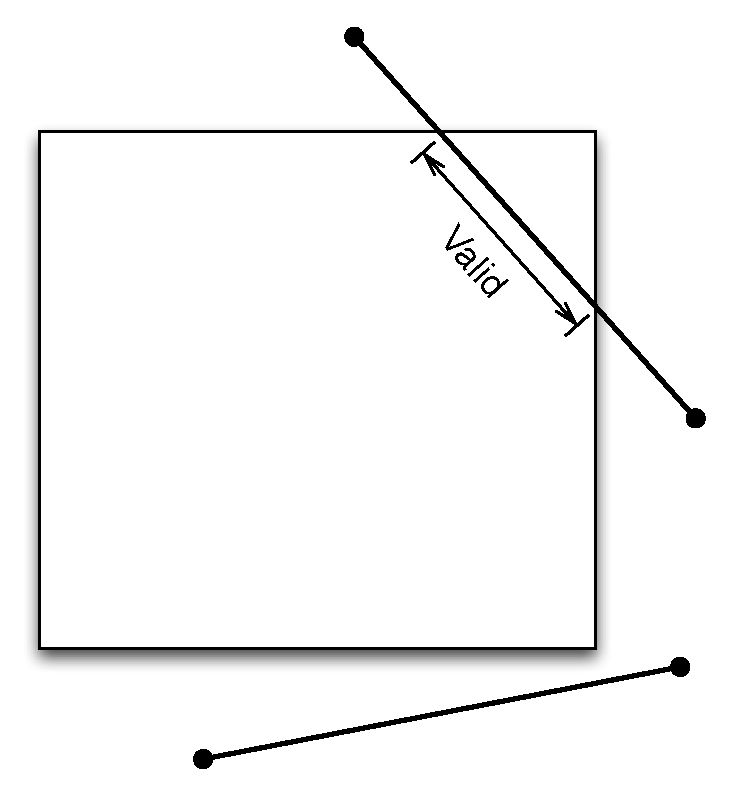
\includegraphics[width=6cm,clip]{Invalid_case.eps}
\end{center}
\caption{ラインのサンプリング指定で無効なケース}
\label{fig:invalid_case}
\end{figure}


%%
\subsection{出力ファイルフォーマット}
採取された物理量は,グループ毎にファイルに出力されます.
出力ファイルは,テキストファイルで,
モニタ点座標とモニタ変数を記述した{\bf ヘッダ領域}と,それに続く,
採取したステップ数個の{\bf データ領域}からなります.
ヘッダ領域とデータ領域,および,隣接するデータ領域間は1行の空行で区切られています.

\paragraph{ヘッダ領域}
1行目の整数nにモニタ点数と,モニタ対象の物理量を示すキーワード(Velocity, Presure等)が並びます.
続くn行に,各モニタ点の座標値およびcommentが出力されます.
なお,分散出力時には,nは担当ノード内のモニタ点数になり,担当モニタ点の座標値のみを出力します.
\begin{center}
\vspace{0.2\baselineskip}
\begin{tabular}{|p{14em}|p{20em}}\cline{1-1}
n Velocity Presure Temperature  & ← n点で速度,圧力,温度をモニタ\\ 
$x_1$  $y_1$  $z_1$  \#comment  & ← 各モニタ点の座標とcommentを\\
$x_2$  $y_2$  $z_2$  \#comment  &  空白区切りで出力\\
  …                   & \\
$x_n$ $y_n$ $z_n$    \#comment & \\
\cline{1-1}
\end{tabular}
\vspace{0.2\baselineskip}
\end{center}

\paragraph{データ領域}
1行目に,採取時のステップ数step(整数)とソルバー内部時間time(実数)が出力されます.
続くn行に,各モニタ点で採取した値が,ヘッダ領域のキーワードの並び順に出力されます.
\begin{center}
\vspace{0.2\baselineskip}
\begin{tabular}{|p{14em}|p{20em}}\cline{1-1}
step time  & ← ステップ数=step, 時間=time\\ 
$u_1$  $v_1$  $w_1$ $p_1$ $t_1$  & ← モニタ点毎の採取値が\\
$u_2$  $v_2$  $w_2$ $p_2$ $t_2$  &   空白区切りで並ぶ\\
  …                             &   ($u_i,v_i,w_i$)=速度,$p_i$=圧力,$t_i$=温度\\
$u_n$ $v_n$ $w_n$ $p_n$ $t_n$  & \\
\cline{1-1}
\end{tabular}
\vspace{0.2\baselineskip}
\end{center}

採取値の有効桁数は,単精度計算では小数点以下7桁,倍精度計算では16桁です.

なお,採取モードの制限により採取をスキップされたモニタ点では,データ領域の該当する行には,「*NA*」の文字列が出力されます.


%%%
\pagebreak
\hypertarget{tgt:cell_monitor}{\section{ボクセルモデルのセルIDで指定する方法}}
セルIDにより指定する方法は,各セル中心をモニタ点として,
sampling\_method=\lq\lq nearest\rq\rq , sampling\_mode=\lq\lq all\rq\rq の条件で採取を行います.

%
\subsection{モニター部の指定}
計算領域の内部において,物理量をモニタしたい部分をボクセルモデルのセルIDにより指定します.
モニタ面は基本的には,座標軸に面直な面とします.
ただし,若干予測精度は低下するが,軸に対して斜めの領域も指定できます.
condition.txt内のComponent Informationの部分にモニタ面の推定法線と面積の情報が表示されるので,確認してください.
ひとつのIDに対しては,単連結領域(一つの塊)となるようにIDを割り当てる必要があります.

\vspace{5mm}
\begin{indentation}{2zw}{0zw}

下記の例では,ID=20で指定される領域をモニタ部とし,そこで速度,圧力,全圧をモニタすることを指定しています.モニタ面の法線を指定しています.

{\small
\begin{program}
<InnerBoundary>
  <Elem name="Cell_Monitor" id="20" comment="monitor_inlet"> 
    <Param name="Normal_x" dtype="REAL" value="1.0" /> 
    <Param name="Normal_y" dtype="REAL" value="0.0" /> 
    <Param name="Normal_z" dtype="REAL" value="0.0" /> 
    <Elem name="Variables"> 
      <Param name="velocity"       dtype="STRING" value="on" /> 
      <Param name="pressure"       dtype="STRING" value="on" /> 
      <Param name="temperature"    dtype="STRING" value="off" /> 
      <Param name="Total_pressure" dtype="STRING" value="on" /> 
    </Elem> 
  </Elem>
</InnerBoundary>
\end{program}
}

\end{indentation}


%%%
\pagebreak
\section{モニター例}
以下の指定によって,10ステップ毎にサンプリングする例を示します.

\begin{quote}
\begin{description}
\item[line ``Lx'']  x軸にそって5点($x=-0.5$, $-0.25$, $0.0$, $0.25$, $0.5$)
\item[line ``Ly'']  y軸にそって5点($y=-0.5$, $-0.25$, $0.0$, $0.25$, $0.5$)
\item[line ``Lz'']  z軸にそって5点($z=-0.5$, $-0.25$, $0.0$, $0.25$, $0.5$)
\item[point\_set ``P8''] $x=\pm0.25$, $y=\pm0.25$, $z=\pm0.25$の組み合わせで8点
\end{description}
\end{quote}

{\small
\begin{program}
<Elem name="Monitor_List">
   <Param name="Log"                    dtype="STRING" value="On" />
   <Param name="output_mode"            dtype="string" value="Gather" />
   <Param name="Unit"                   dtype="STRING" value="Non_Dimensional" />
   <Param name="Sampling_Interval_Type" dtype="string" value="Step" />
   <Param name="Sampling_Interval"      dtype="real"   value="10" />
 
   <Elem name="line" comment="Lx">
     <Param name="variable"   dtype="string"   value="velocity" />
     <Param name="variable"   dtype="string"   value="pressure" />
     <Param name="sampling_method" dtype="string" value="interpolation" />
     <Param name="sampling_mode"   dtype="string" value="fluid" />
     <Param name="division"   dtype="int"   value="4" />
     <Elem name="from">
       <Param name="x"   dtype="REAL"   value="-0.5" />
       <Param name="y"   dtype="REAL"   value="0.0" />
       <Param name="z"   dtype="REAL"   value="0.0" />
     </Elem>
     <Elem name="to">
       <Param name="x"   dtype="REAL"   value="0.5" />
       <Param name="y"   dtype="REAL"   value="0.0" />
       <Param name="z"   dtype="REAL"   value="0.0" />
     </Elem>
   </Elem>
      
   <Elem name="line" comment="Lz">
     <Param name="variable"   dtype="string"   value="velocity" />
     <Param name="variable"   dtype="string"   value="pressure" />
     <Param name="sampling_method" dtype="string" value="interpolation" />
     <Param name="sampling_mode"   dtype="string" value="fluid" />
     <Param name="division"   dtype="int"   value="4" />
     <Elem name="from">
       <Param name="x"   dtype="REAL"   value="0.0" />
       <Param name="y"   dtype="REAL"   value="0.0" />
       <Param name="z"   dtype="REAL"   value="-0.5" />
     </Elem>
     <Elem name="to">
       <Param name="x"   dtype="REAL"   value="0.0" />
       <Param name="y"   dtype="REAL"   value="0.0" />
       <Param name="z"   dtype="REAL"   value="0.5" />
     </Elem>
   </Elem>

   <Elem name="line" comment="Ly">
     <Param name="variable"   dtype="string"   value="velocity" />
     <Param name="variable"   dtype="string"   value="pressure" />
     <Param name="sampling_method" dtype="string" value="interpolation" />
     <Param name="sampling_mode"   dtype="string" value="fluid" />
     <Param name="division"   dtype="int"   value="4" />
     <Elem name="from">
       <Param name="x"   dtype="REAL"   value="0.0" />
       <Param name="y"   dtype="REAL"   value="-0.5" />
       <Param name="z"   dtype="REAL"   value="0.0" />
     </Elem>
     <Elem name="to">
       <Param name="x"   dtype="REAL"   value="0.0" />
       <Param name="y"   dtype="REAL"   value="0.5" />
       <Param name="z"   dtype="REAL"   value="0.0" />
     </Elem>
   </Elem>

   <Elem name="point_set" comment="P8">
     <Param name="variable"   dtype="string"   value="pressure" />
     <Param name="variable"   dtype="string"   value="velocity" />
     <Param name="variable"   dtype="string"   value="vorticity" />
     <Param name="sampling_method" dtype="string" value="smoothing" />
     <Param name="sampling_mode"   dtype="string" value="fluid" />
     <Elem name="set" comment="[- - -]">
       <Param name="x"   dtype="REAL"   value="-0.25" />
       <Param name="y"   dtype="REAL"   value="-0.25" />
       <Param name="z"   dtype="REAL"   value="-0.25" />
     </Elem>
     <Elem name="set" comment="[+ - -]">
       <Param name="x"   dtype="REAL"   value=" 0.25" />
       <Param name="y"   dtype="REAL"   value="-0.25" />
       <Param name="z"   dtype="REAL"   value="-0.25" />
     </Elem>
     <Elem name="set" comment="[- + -]">
       <Param name="x"   dtype="REAL"   value="-0.25" />
       <Param name="y"   dtype="REAL"   value=" 0.25" />
       <Param name="z"   dtype="REAL"   value="-0.25" />
     </Elem>
     <Elem name="set" comment="[+ + -]">
       <Param name="x"   dtype="REAL"   value=" 0.25" />
       <Param name="y"   dtype="REAL"   value=" 0.25" />
       <Param name="z"   dtype="REAL"   value="-0.25" />
     </Elem>
     <Elem name="set" comment="[- - +]">
       <Param name="x"   dtype="REAL"   value="-0.25" />
       <Param name="y"   dtype="REAL"   value="-0.25" />
       <Param name="z"   dtype="REAL"   value=" 0.25" />
     </Elem>
     <Elem name="set" comment="[+ - +]">
       <Param name="x"   dtype="REAL"   value=" 0.25" />
       <Param name="y"   dtype="REAL"   value="-0.25" />
       <Param name="z"   dtype="REAL"   value=" 0.25" />
     </Elem>
     <Elem name="set" comment="[- + +]">
       <Param name="x"   dtype="REAL"   value="-0.25" />
       <Param name="y"   dtype="REAL"   value=" 0.25" />
       <Param name="z"   dtype="REAL"   value=" 0.25" />
     </Elem>
     <Elem name="set" comment="[+ + +]">
       <Param name="x"   dtype="REAL"   value=" 0.25" />
       <Param name="y"   dtype="REAL"   value=" 0.25" />
       <Param name="z"   dtype="REAL"   value=" 0.25" />
     </Elem>
   </Elem>
      
   <InnerBoundary>
     <Elem name="Cell_Monitor" id="20" comment="monitor_inlet"> 
       <Param name="reference" dtype="string" value="no" /> 
       <Param name="Norm_x" dtype="REAL" value="1.0" /> 
       <Param name="Norm_y" dtype="REAL" value="0.0" /> 
       <Param name="Norm_z" dtype="REAL" value="0.0" /> 
       <Elem name="Variables"> 
         <Param name="velocity" dtype="STRING" value="on" /> 
         <Param name="pressure" dtype="STRING" value="on" /> 
         <Param name="temperature" dtype="STRING" value="off" /> 
         <Param name="Total_pressure" dtype="STRING" value="on" /> 
       </Elem> 
     </Elem>
   </InnerBoundary>
\end{program}
}

%%
\pagebreak
\subsection{初期化時の出力情報}
以下に,4並列実行時の出力例を示します.

{\small
\begin{program}
>> Monitor Information

  Output Type : Gather

  1 : Line   division=5  [Lx]
    Variables : Velocity Pressure 
       Method : Interpolation
         Mode : All
        order :            X            Y            Z  :   rank : comment
            1 :  -5.0000e-01   0.0000e+00   0.0000e+00  :      3 : point_0
            2 :  -2.5000e-01   0.0000e+00   0.0000e+00  :      3 : point_1
            3 :   0.0000e+00   0.0000e+00   0.0000e+00  :      3 : point_2
            4 :   2.5000e-01   0.0000e+00   0.0000e+00  :      3 : point_3
            5 :   5.0000e-01   0.0000e+00   0.0000e+00  :      3 : point_4

  2 : Line   division=5  [Lz]
    Variables : Velocity Pressure 
       Method : Interpolation
         Mode : All
        order :            X            Y            Z  :   rank : comment
            1 :   0.0000e+00   0.0000e+00  -5.0000e-01  :      1 : point_0
            2 :   0.0000e+00   0.0000e+00  -2.5000e-01  :      1 : point_1
            3 :   0.0000e+00   0.0000e+00   0.0000e+00  :      3 : point_2
            4 :   0.0000e+00   0.0000e+00   2.5000e-01  :      3 : point_3
            5 :   0.0000e+00   0.0000e+00   5.0000e-01  :      3 : point_4

  3 : Line   division=5  [Ly]
    Variables : Velocity Pressure 
       Method : Interpolation
         Mode : All
        order :            X            Y            Z  :   rank : comment
            1 :   0.0000e+00  -5.0000e-01   0.0000e+00  :      2 : point_0
            2 :   0.0000e+00  -2.5000e-01   0.0000e+00  :      2 : point_1
            3 :   0.0000e+00   0.0000e+00   0.0000e+00  :      3 : point_2
            4 :   0.0000e+00   2.5000e-01   0.0000e+00  :      3 : point_3
            5 :   0.0000e+00   5.0000e-01   0.0000e+00  :      3 : point_4

  4 : Point_set  division=8  [P8]
    Variables : Velocity Pressure Vorticity 
       Method : Smoothing
         Mode : All
        order :            X            Y            Z  :   rank : comment
            1 :  -2.5000e-01  -2.5000e-01  -2.5000e-01  :      0 : [- - -]
            2 :   2.5000e-01  -2.5000e-01  -2.5000e-01  :      0 : [+ - -]
            3 :  -2.5000e-01   2.5000e-01  -2.5000e-01  :      1 : [- + -]
            4 :   2.5000e-01   2.5000e-01  -2.5000e-01  :      1 : [+ + -]
            5 :  -2.5000e-01  -2.5000e-01   2.5000e-01  :      2 : [- - +]
            6 :   2.5000e-01  -2.5000e-01   2.5000e-01  :      2 : [+ - +]
            7 :  -2.5000e-01   2.5000e-01   2.5000e-01  :      3 : [- + +]
            8 :   2.5000e-01   2.5000e-01   2.5000e-01  :      3 : [+ + +]

  5 : Inner Boundary     division=4  [InnerBoundary1]
    Variables : Velocity Pressure 
       Method : Nearest
         Mode : All
        order :            X            Y            Z  :   rank : comment
            1 :  -7.8125e-03  -7.8125e-03  -7.8125e-03  :      0 : point_0
            2 :  -7.8125e-03   7.8125e-03  -7.8125e-03  :      1 : point_1
            3 :  -7.8125e-03  -7.8125e-03   7.8125e-03  :      2 : point_2
            4 :  -7.8125e-03   7.8125e-03   7.8125e-03  :      3 : point_3
\end{program}
}

%%
\subsection{単一ファイル出力}
以下は,4並列実行時のファイル出力内容(monitor\_Lz.log)です.
最初の6行はヘッダで,5点のモニタ点(2$\sim$6行目に座標とラベルが示されています)に対して,速度($u,v,w$3成分)と圧力をモニタすることがわかります.
各ステップのモニタ値にはステップ数と時刻のヘッダがつきます.

{\small
\begin{program}
5 Velocity Pressure 
  0.0000e+00   0.0000e+00  -5.0000e-01  #point_0
  0.0000e+00   0.0000e+00  -2.5000e-01  #point_1
  0.0000e+00   0.0000e+00   0.0000e+00  #point_2
  0.0000e+00   0.0000e+00   2.5000e-01  #point_3
  0.0000e+00   0.0000e+00   5.0000e-01  #point_4

10   3.1250e-02
  0.0000000e+00   0.0000000e+00   0.0000000e+00   0.0000000e+00 
  0.0000000e+00   0.0000000e+00   0.0000000e+00   0.0000000e+00 
  0.0000000e+00   0.0000000e+00   0.0000000e+00   0.0000000e+00 
 -9.4408710e-26   0.0000000e+00  -1.4733364e-32   1.2573367e-32 
  1.0951646e-04   0.0000000e+00   7.5170038e-23  -1.3972461e-21 

20   6.2500e-02
 -1.2704001e-14  -3.9074446e-19  -1.3234890e-21   7.5723732e-20 
 -1.0800631e-10  -3.4509484e-15   1.3357371e-16  -1.0019127e-15 
 -4.8423708e-08  -1.4604844e-12   2.6645353e-13  -3.1363824e-12 
 -1.4771770e-06  -3.9237082e-11   2.1965540e-11  -3.6127115e-10 
  7.4478355e-04  -5.5457045e-11   4.2911008e-11  -2.1239641e-09 

30   9.3750e-02
 -3.5265384e-07  -3.4598248e-11  -1.2434498e-13   4.3679508e-11 
 -4.3679470e-06  -2.3597949e-10  -3.1370462e-12   2.8554661e-10 
 -2.3169587e-05  -5.8292204e-10   2.8683900e-10  -2.2359627e-09 
 -6.6163069e-05  -8.1312534e-10   2.1909443e-09  -2.8697086e-08 
  2.2175554e-03  -3.7072784e-10   8.8358654e-10  -4.6022318e-08 

…
\end{program}
}

%%
\subsection{分散ファイル出力}
前述と同条件でのファイル出力例(monitor\_Lz\_1.log)です.

{\small
\begin{program}
2 Velocity Pressure 
  0.0000e+00   0.0000e+00  -5.0000e-01  #point_0
  0.0000e+00   0.0000e+00  -2.5000e-01  #point_1

10   3.1250e-02
  0.0000000e+00   0.0000000e+00   0.0000000e+00   0.0000000e+00 
  0.0000000e+00   0.0000000e+00   0.0000000e+00   0.0000000e+00 

20   6.2500e-02
 -1.2704001e-14  -3.9074446e-19  -1.3234890e-21   7.5723732e-20 
 -1.0800631e-10  -3.4509484e-15   1.3357371e-16  -1.0019127e-15 

30   9.3750e-02
 -3.5265384e-07  -3.4598248e-11  -1.2434498e-13   4.3679508e-11 
 -4.3679470e-06  -2.3597949e-10  -3.1370462e-12   2.8554661e-10

…
\end{program}
}

%%
\pagebreak
\subsection{Sampling\_Modeの指定例}
全グループでSampling\_Mode=\lq\lq fluid\rq\rq とした場合の初期化時のコンソール出力です.

{\small
\begin{program}
>> Monitor Information

  Output Type : Gather

  1 : Line   division=5  [Lx]
    Variables : Velocity Pressure 
       Method : Interpolation
         Mode : Fluid
        order :            X            Y            Z  :   rank : comment
            1 :  -5.0000e-01   0.0000e+00   0.0000e+00  :      3 : point_0
            2 :  -2.5000e-01   0.0000e+00   0.0000e+00  :      3 : point_1
            3 :   0.0000e+00   0.0000e+00   0.0000e+00  :      3 : point_2
            4 :   2.5000e-01   0.0000e+00   0.0000e+00  :      3 : point_3
            5 :   5.0000e-01   0.0000e+00   0.0000e+00  :      3 : point_4  *
skip(unexpected solid)*

  2 : Line   division=5  [Lz]
    Variables : Velocity Pressure 
       Method : Interpolation
         Mode : Fluid
        order :            X            Y            Z  :   rank : comment
            1 :   0.0000e+00   0.0000e+00  -5.0000e-01  :      1 : point_0
            2 :   0.0000e+00   0.0000e+00  -2.5000e-01  :      1 : point_1
            3 :   0.0000e+00   0.0000e+00   0.0000e+00  :      3 : point_2
            4 :   0.0000e+00   0.0000e+00   2.5000e-01  :      3 : point_3
            5 :   0.0000e+00   0.0000e+00   5.0000e-01  :      3 : point_4  *
skip(unexpected solid)*

  3 : Line   division=5  [Ly]
    Variables : Velocity Pressure 
       Method : Interpolation
         Mode : Fluid
        order :            X            Y            Z  :   rank : comment
            1 :   0.0000e+00  -5.0000e-01   0.0000e+00  :      2 : point_0
            2 :   0.0000e+00  -2.5000e-01   0.0000e+00  :      2 : point_1
            3 :   0.0000e+00   0.0000e+00   0.0000e+00  :      3 : point_2
            4 :   0.0000e+00   2.5000e-01   0.0000e+00  :      3 : point_3
            5 :   0.0000e+00   5.0000e-01   0.0000e+00  :      3 : point_4  *
skip(unexpected solid)*

  4 : Point_set  division=8  [P8]
    Variables : Velocity Pressure Vorticity 
       Method : Smoothing
         Mode : Fluid
        order :            X            Y            Z  :   rank : comment
            1 :  -2.5000e-01  -2.5000e-01  -2.5000e-01  :      0 : [- - -]
            2 :   2.5000e-01  -2.5000e-01  -2.5000e-01  :      0 : [+ - -]
            3 :  -2.5000e-01   2.5000e-01  -2.5000e-01  :      1 : [- + -]
            4 :   2.5000e-01   2.5000e-01  -2.5000e-01  :      1 : [+ + -]
            5 :  -2.5000e-01  -2.5000e-01   2.5000e-01  :      2 : [- - +]
            6 :   2.5000e-01  -2.5000e-01   2.5000e-01  :      2 : [+ - +]
            7 :  -2.5000e-01   2.5000e-01   2.5000e-01  :      3 : [- + +]
            8 :   2.5000e-01   2.5000e-01   2.5000e-01  :      3 : [+ + +]

  5 : Inner Boundary     division=4  [InnerBoundary1]
    Variables : Velocity Pressure 
       Method : Nearest
         Mode : All
        order :            X            Y            Z  :   rank : comment
            1 :  -7.8125e-03  -7.8125e-03  -7.8125e-03  :      0 : point_0
            2 :  -7.8125e-03   7.8125e-03  -7.8125e-03  :      1 : point_1
            3 :  -7.8125e-03  -7.8125e-03   7.8125e-03  :      2 : point_2
            4 :  -7.8125e-03   7.8125e-03   7.8125e-03  :      3 : point_3
\end{program}
}

上例のlineグループのように,線分の端点が計算対象領域境界上にある場合には,そのモニタ点がガイドセル側に属すると判断されることがあります.
Sampling\_Mode=\lq\lq fluid\rq\rq と指定したにもかかわらずモニタ点を含むセルが固体セルであるため,警告メッセージ「{\tt  *skip(unexpected solid)*}」が出力される場合があります.

この現象を防止するために,lineグループ指定時の線分端点座標を,常に実際の計算対象領域よりわずかに小さい領域にクリッピングする仕様としています.
したがって,上記の警告メッセージはでないはずです.


\subsection{スキップモニタ点がある場合のファイル出力例(単一ファイル)}
上と同条件の計算でのファイル出力(monitor\_Lz.log)です.

{\small
\begin{program}
5 Velocity Pressure 
  0.0000e+00   0.0000e+00  -5.0000e-01  #point_0
  0.0000e+00   0.0000e+00  -2.5000e-01  #point_1
  0.0000e+00   0.0000e+00   0.0000e+00  #point_2
  0.0000e+00   0.0000e+00   2.5000e-01  #point_3
  0.0000e+00   0.0000e+00   5.0000e-01  #point_4  *skip(unexpected solid)*

10   3.1250e-02
  0.0000000e+00   0.0000000e+00   0.0000000e+00   0.0000000e+00 
  0.0000000e+00   0.0000000e+00   0.0000000e+00   0.0000000e+00 
  0.0000000e+00   0.0000000e+00   0.0000000e+00   0.0000000e+00 
 -9.4408710e-26   0.0000000e+00  -1.4733364e-32   1.2573367e-32 
  *NA*

20   6.2500e-02
 -2.3736999e-14  -1.1059020e-18  -1.2751029e-15   7.6158697e-14 
 -1.0800631e-10  -3.4509484e-15   1.3357371e-16  -1.0019127e-15 
 -4.8423708e-08  -1.4604844e-12   2.6645353e-13  -3.1363824e-12 
 -1.4771770e-06  -3.9237082e-11   2.1965540e-11  -3.6127115e-10 
  *NA*

30   9.3750e-02
 -7.0001181e-07  -8.6439161e-11  -1.8219026e-09   1.1022797e-06 
 -4.3679470e-06  -2.3597949e-10  -3.1370462e-12   2.8554661e-10 
 -2.3169587e-05  -5.8292204e-10   2.8683900e-10  -2.2359627e-09 
 -6.6163069e-05  -8.1312534e-10   2.1909443e-09  -2.8697086e-08 
  *NA*

…
\end{program}
}




%%%
\chapter{ソルバーの実行}

\begin{abstract}
FFV-Cソルバーの実行方法と出力ファイルについて説明します.
\end{abstract}
%
\graphicspath{{./fig_Exec/}}
%

\section{FFV-Cソルバーの実行}

次のようなディレクトリ構成を仮定し,3Dcavityの例題を実行します.
標準のMakefileでコンパイルすると,コンパイル済みの実行モジュールはbinディレクトリに格納されます.
パラメータファイルは,\verb|cavity.tp, domain.tp|とします.

{\small
\begin{program}
Examples
  |
  +- 3Dcavity
  |    +-cavity.tp
  :
\end{program}
}

カレントディレクトリをExamples/3Dcavityとし,実行モジュールのディレクトリにパスを通しておくと,以下のように実行できます.

{\small
\begin{program}
$ ffvc cavity.tp domain.tp
\end{program}
}

%
\pagebreak
\section{出力ファイル}

\subsection{出力ファイルの種類と指定}
\label{sec:log_files}

FFV-Cソルバーを実行すると,\textbf{表\ref{tbl:logfiles}}に示すファイルが生成されます.
また,logファイルについては,\hyperlink{tgt:log}{Log}セクションで生成の有無を指定します.

\begin{table}[htdp]
\caption{実行時に生成されるファイル}
\begin{center}
\small
\begin{tabular}{lll}\toprule
カテゴリ & ファイル名 & 出力内容\\ \midrule
解析条件情報 & \verb|condition.txt| & 計算条件,前処理,ソルバー起動時のログ\\
領域情報 & \verb|DomainInfo.txt| & 並列計算時の計算領域の分割に関する情報\\ 
性能情報 & \verb|profiling.txt| & 実行時間サンプリング出力ファイル\\ \hline
基本履歴 & \verb|history_base.txt| & ステップ数,時刻,反復回数,収束状況などの情報\\
コンポーネント履歴 & \verb|history_compo.txt| & 内部境界のモニタ情報\\
流量収支履歴 & \verb|history_domainflux.txt| & 計算外部領域における流入出流量,平均速度の情報\\
反復履歴 & \verb|history_iteration.txt| & 反復解法の収束履歴\\ 
サンプリング履歴 & \verb|sampling.txt| & サンプリング指定時の出力ファイル\\ 
壁面情報履歴 & \verb|history_log_wall.txt| & 壁面に関する情報の履歴\\ \hline
瞬時値データ & \verb|vel_*.sph| & 速度の瞬時値\\
& \verb|prs_*.sph| & 圧力の瞬時値\\
& \verb|tmp_*.sph| & 温度の瞬時値\\
平均値データ & \verb|vela_*.sph| & 速度の時間平均値\\
& \verb|prsa_*.sph| & 圧力の時間平均値\\
& \verb|tmpa_*.sph| & 温度の時間平均値\\
派生データ & \verb|tp_*.sph| & 全圧\\
& \verb|vrt_*.sph| & 渦度\\
& \verb|hlt_*.sph| & ヘリシティ\\
& \verb|i2vgt_*.sph| & 速度勾配テンソルの第2不変量\\ 
\bottomrule
\end{tabular}
\end{center}
\label{tbl:logfiles}
\end{table}

\textbf{表\ref{tbl:logfiles}}の履歴と瞬時値・平均値のデータ出力については,出力インターバルを指定できます.
出力インターバルは\hyperlink{tgt:fileio}{File\_IO}セクションに記述し,各項目独立に,ステップと時刻のどちらによっても指定可能です.
ファイル名のアスタリスク\verb|*|には,ステップ数やランク番号などの情報が入ります.また,拡張子の\verb|.sph|はsph形式を表しており,PLOT3Dフォーマットもサポートします.

%
\pagebreak
\subsection{解析条件情報 [condition.txt]}

ソルバーを実行すると,\verb|condition.txt|ファイル\index{ふぁいる@ファイル!condition---}が生成されます.
このファイルはソルバーの起動時のログで,必要な境界条件の設定に係わる前処理,チェック内容などが\textbf{表\ref{tbl:log-section}}に示す各セクション毎に記録されています.

\begin{table}[htdp]
\caption{condition.txtファイルの表示項目}
\begin{center}
\small
\begin{tabular}{ll}\toprule
セクション名 & 表示内容\\ \midrule
Domain Information & 計算領域の寸法,配列サイズ,格子ピッチ,原点座標\\
Memory required for Preprocesor & 前処理に必要なメモリ要求量(概算)\\
XML Components & コンポーネントの種類と個数\\
Voxel Model Info. & 解析モデルに含まれる情報\\
Medium List & 媒質情報\\
Component List & 各コンポーネントのID,要素数,媒質など\\
Component Information & 各コンポーネントの詳細な情報\\
Memory required for Solver & ソルバー本体で必要なメモリ要求量(概算)\\
Solver Control Parameters & 制御パラメータ\\
Simulation Parameters & 物理量のパラメータ\\
Initial Values for Physical Variables & 初期値の情報\\
Effective cells and Open Area of Computational Domain& 計算対象セル数と各外部境界面における開口面積の割合\\
Outer Boundary Conditions & 外部境界条件\\ 
Monitor Information & モニター情報\\ \bottomrule
\end{tabular}
\end{center}
\label{tbl:log-section}
\end{table}


%
\pagebreak
\subsection{領域情報 [DomainInfo.txt]}
領域全体の情報,および領域分割された各サブドメインの配列サイズ,領域サイズ,原点座標の情報が表示されます.
また,各領域に含まれる境界条件コンポーネントのBoundingBoxのインデクス情報が含まれます.

\begin{indentation}{2zw}{0zw}
{\small 
\begin{program}
>> Global Domain Information

imax, jmax, kmax    =            73            28            28

(dx, dy, dz) [m] / [-] = ( 2.0000e-02 2.0000e-02 2.0000e-02) / ( 3.5714e-02 3.5714e-02 3.5714e-02)
(ox, oy, oz) [m] / [-] = ( 2.0000e-02 2.0000e-02 2.0000e-02) / ( 3.5714e-02 3.5714e-02 3.5714e-02)
(Lx, Ly, Lz) [m] / [-] = ( 1.4600e+00 5.6000e-01 5.6000e-01) / ( 2.6071e+00 1.0000e+00 1.0000e+00)

Domain    0
ix, jx,  kx        [-] =             37            28            28
(ox, oy, oz) [m] / [-] = ( 2.0000e-02 2.0000e-02 2.0000e-02) / ( 3.5714e-02 3.5714e-02 3.5714e-02)
(Lx, Ly, Lz) [m] / [-] = ( 7.4000e-01 5.6000e-01 5.6000e-01) / ( 1.3214e+00 1.0000e+00 1.0000e+00)
no            Label    ID    i_st    i_ed    j_st    j_ed    k_st    k_ed
 1              Air     4       0       0       0       0       0       0

Domain    1
ix, jx,  kx        [-] =             36            28            28
(ox, oy, oz) [m] / [-] = ( 7.6000e-01 2.0000e-02 2.0000e-02) / ( 1.3571e+00 3.5714e-02 3.5714e-02)
(Lx, Ly, Lz) [m] / [-] = ( 7.1999e-01 5.6000e-01 5.6000e-01) / ( 1.2857e+00 1.0000e+00 1.0000e+00)
no            Label    ID    i_st    i_ed    j_st    j_ed    k_st    k_ed
 1              Air     4      14      17       1      28       1      28
\end{program}
}
\end{indentation} 



%
\pagebreak
\subsection{基本履歴 [history\_base.txt]}
\label{sec:baseinfo}

標準履歴ファイル\index{ふぁいる@ファイル!ひょうじゅんりれき@標準履歴---}は,下記のような履歴情報\index{りれき@履歴}が出力されます.
この履歴情報は選択された時間積分スキームや反復解法の収束判定ノルムの種類などにより出力項目は異なります.
下記の計算例では,時間積分にEuler陽解法を用いた流動解析を行い,圧力Poisson方程式の反復解の収束判定のノルムに速度の発散の最大値を用いています.
各欄のラベルの説明を\textbf{表\ref{tbl:out_label}}に示します.

標準出力とhistory\_base.logファイルには同じ内容が出力され,時刻と速度の次元は有次元となっています.収束判定のノルムの種類については,\textbf{表\ref{tbl:norm-type}}を参照のこと.ノルムの次元は慣例的に無次元としています.\\

\begin{indentation}{2zw}{0zw}
{\small 
\begin{program}
    step      time[sec]  v_max[m/s]   ItrP   V_div_Max     deltaP       avrP     deltaV       avrV
       1   4.000000e-05  0.0000e+00      1  2.3687e-07  1.476e-14 -7.991e-17  5.493e-15  5.493e-15
       2   8.000001e-05  6.8344e-13      1  1.1870e-06  2.602e-09  1.069e-10  1.878e-10  1.878e-10
       3   1.200000e-04  2.4322e-08      1  2.8058e-06  9.901e-09  5.841e-10  8.173e-10  1.003e-09
       4   1.600000e-04  1.1977e-07      1  4.6971e-06  2.073e-08  1.737e-09  1.942e-09  2.937e-09
       5   2.000000e-04  3.2279e-07      1  6.7086e-06  3.395e-08  3.859e-09  3.487e-09  6.404e-09
       6   2.400000e-04  6.6904e-07      1  8.8056e-06  4.920e-08  7.234e-09  5.350e-09  1.171e-08
       7   2.800000e-04  1.1826e-06      1  1.0970e-05  6.639e-08  1.214e-08  7.459e-09  1.910e-08
\end{program}
}

\begin{table}[htdp]
\caption{履歴ファイルの出力項目}
\begin{center}
\small
\begin{tabular}{ll} \toprule
Label & 説明\\ \midrule
step & 計算ステップ数\\
time & 時刻\\
v\_max & 速度の最大値\\
ItrP & 圧力ポアソンの反復回数\\
V\_div\_Max & 反復の収束判定に用いるノルムの種類とその値.上記の場合は速度の発散値の最大値を用いています.\\
& 指定するノルムの種類により,ヘッダの記述が変わります.\\
deltaP & 圧力の1ステップの変化量の自乗和平方根 $\sqrt{ \sum_{i,j,k}^{Max} {\|\delta{p}\|}_{2} }$\\
avrP   & 圧力の平均値\\
deltaV & 速度の1ステップの変化量の自乗和平方根 $\sqrt{ \sum_{i,j,k}^{Max} {\|\delta{v}\|}_{2} }$\\
avrV   & 速度の平均値\\
deltaT & 温度の1ステップの変化量の自乗和平方根 $\sqrt{ \sum_{i,j,k}^{Max} {\|\delta{\theta}\|}_{2} }$\\ 
avrT   & 温度の平均値\\ \bottomrule
\end{tabular}
\end{center}
\label{tbl:out_label}
\end{table}


下記には,熱流動計算を流動計算にEuler陽解法,温度場は対流項にEuler陽解法,拡散項にEuler陰解法を用いた履歴の出力例を示す.ItrTは温度の反復解法の反復回数を示し,続くT\_Res\_L2\_Rはノルムに相対残差を選択していることを示します.また,dTは温度の1ステップの変化量のRMSです.

{\small
\begin{program}
step       time       v_max  ItrP P_res_L2_R ItrT T_res_L2_R        dP        dV        dT
   1 1.2500e-04  0.0000e+00     1 0.0000e+00    6 9.5454e-05 0.000e+00 0.000e+00 2.654e-01 
   2 2.5000e-04  0.0000e+00   201 5.2254e-05   11 2.1408e-05 3.962e+05 1.338e+02 2.583e-01 
   3 3.7500e-04  1.0464e+01   201 4.3515e-05    9 8.5652e-05 3.901e+05 2.599e+02 2.495e-01 
   4 5.0000e-04  3.0324e+01   201 3.5191e-05    9 2.8809e-05 3.839e+05 3.750e+02 2.386e-01 
   5 6.2500e-04  5.7543e+01   201 2.8940e-05    8 6.5638e-05 3.789e+05 4.750e+02 2.269e-01 
   6 7.5000e-04  9.2345e+01   201 2.5224e-05    8 3.7452e-05 3.769e+05 5.584e+02 2.164e-01 
   7 8.7500e-04  1.3304e+02   201 2.3655e-05    8 2.4891e-05 3.797e+05 6.287e+02 2.091e-01
\end{program}
}

\end{indentation}


\pagebreak
%
\hypertarget{tgt:history_compo}{\subsection{コンポーネント履歴 [history\_compo.txt]}}

コンポーネントに関連する履歴\index{ふぁいる@ファイル!こんぽーねんとりれき@コンポーネント履歴---}を出力します.

\begin{indentation}{2zw}{0zw}
{\small 
\begin{program}
    step         time    V[inlet]     Va[hex]    DPa[hex]  MonV[sensor]  MonP[sensor] MonTP[sensor]
       1   2.9605e-03 -1.6511e-02  0.0000e+00  0.0000e+00    0.0000e+00    1.0132e+05    0.0000e+00
       2   5.9211e-03 -6.6040e-02  0.0000e+00  0.0000e+00    0.0000e+00    1.0132e+05    0.0000e+00
       3   8.8816e-03 -1.4857e-01  0.0000e+00  0.0000e+00    0.0000e+00    1.0132e+05    0.0000e+00
       4   1.1842e-02 -2.6406e-01  0.0000e+00  0.0000e+00    0.0000e+00    1.0132e+05    0.0000e+00
       5   1.4803e-02 -4.1247e-01  0.0000e+00  0.0000e+00    0.0000e+00    1.0132e+05    0.0000e+00
       6   1.7763e-02 -5.9375e-01  0.0000e+00  0.0000e+00    0.0000e+00    1.0132e+05    0.0000e+00
       7   2.0724e-02 -8.0783e-01  0.0000e+00  0.0000e+00    0.0000e+00    1.0132e+05   -2.8205e-33
       8   2.3684e-02 -1.0546e+00  0.0000e+00  0.0000e+00   -7.5572e-24    1.0132e+05   -7.6584e-19
       9   2.6645e-02 -1.3340e+00  0.0000e+00  0.0000e+00   -6.7933e-17    1.0132e+05   -1.3883e-11
      10   2.9605e-02 -1.6460e+00  0.0000e+00  0.0000e+00   -2.4990e-13    1.0132e+05   -7.4992e-08
\end{program}
}

上記の例では,inletに速度を指定し,その平均速度を出力しています.hexには熱交換器を割り当て,平均通過流速と圧力損失量を表示しています.また,sensorはモニタで,平均速度,圧力,全圧を出力しています.各表示量は有次元値で,\textbf{表\ref{tbl:monitor-display}}に示す項目が表示されます.

\begin{table}[htdp]
\caption{コンポーネント履歴ファイルの出力項目}
\begin{center}
\small
\begin{tabular}{lll} \toprule
カテゴリー & コンポーネント & 表示項目\\ \midrule
Vec\_Face & &\\
& Dirichlet & 平均速度 $V\,[m/s]$\\
& & 温度指定の場合,流入熱量 $Q\,[W]$\\
Forcing\_Volume & &\\
& HEX & 熱交換機平均通過流量 $Va\,[m^3/s]$\\
& & 平均圧力損失量 $DPa [Pa]$\\
& DARCY & 平均通過風速の速度成分 $U,\,V,\,W,\,[m/s]$\\
Heat\_Face & &\\
& Direct & 熱流束 $q\,[W/m^2]$\\
& Heat\_Transfer\_N & 熱流束 $q\,[W/m^2]$\\
& Heat\_Transfer\_S & 熱流束 $q\,[W/m^2]$\\
& Heat\_Transfer\_B & 熱流束 $q\,[W/m^2]$\\
& Iso\_Thermal & 熱流束 $q\,[W/m^2]$\\
& Radiation & 熱流束 $q\,[W/m^2]$\\
Heat\_Volume & &\\
& Heat\_Src &\\
& Cnst\_Temp &\\
Monitor & &\\
& Velocity & 平均速度 $MonV\,[m/s]$\\
& Pressure & 平均圧力 $MonP\,[Pa]$\\
& Temperature & 平均温度 $MonT\,[K\,or\,C]$\\
& TotalPressure & 平均全圧 $MonTP\,[Pa]$\\
\bottomrule
\end{tabular}
\end{center}
\label{tbl:monitor-display}
\end{table}

\end{indentation}



%
\pagebreak
\subsection{流量収支履歴 [history\_domainflux.txt]}
計算領域の外部境界における流量と速度の履歴\index{ふぁいる@ファイル!りゅうりょうりれき@流量履歴---}を出力します.
Qは断面流量$[m^3/s]$を,Balanceは計算内部領域への流入出する流量の和を示します.
Vは有効断面平均速度$[m/s]$を表すが,BCで述べるように流出断面を指定している場合には指定される対流速度モードの値となります.

\begin{indentation}{2zw}{0zw}
{\small
\begin{program}
    step         time         Q:X-   ...      Q:Z+ >>      Balance         V:X-   ...   V:Z+
     756 1.890020e+00  -7.5980e-02     -1.3623e-01 >>   6.5136e-01  -1.3155e-03  -8.6816e-04
     757 1.892520e+00  -7.6318e-02     -1.3660e-01 >>   6.5357e-01  -1.3214e-03  -8.7049e-04
     758 1.895020e+00  -7.6656e-02     -1.3696e-01 >>   6.5578e-01  -1.3273e-03  -8.7283e-04
\end{program}
}
\end{indentation}



%
\pagebreak
\subsection{反復履歴 [history\_iteration.txt]}
Poissonの反復履歴\index{ふぁいる@ファイル!はんぷくりれき@反復履歴---}を示します.
ノルムの選択に速度の発散を指定している場合には,計算領域内の位置が出力されます.

\begin{indentation}{2zw}{0zw}
{\small 
\begin{program}
step=               1  time= 6.666667e-03  Itration          Norm (     i,      j,      k)
                                                  1  3.765856e-05 (     5,     46,     92)
step=               2  time= 1.333333e-02  Itration          Norm (     i,      j,      k)
                                                  1  1.076603e-04 (     5,     46,     92)
step=               3  time= 2.000000e-02  Itration          Norm (     i,      j,      k)
                                                  1  1.823895e-04 (     5,     46,     92)
step=               4  time= 2.666667e-02  Itration          Norm (     i,      j,      k)
                                                  1  2.715028e-04 (     5,     46,     92)
step=               5  time= 3.333334e-02  Itration          Norm (     i,      j,      k)
                                                  1  3.676064e-04 (     5,     46,     92)
\end{program}
}
\end{indentation}


%
\pagebreak
\subsection{サンプリング履歴 [sampling.txt]}

座標値指定によるサンプリング結果を出力します.
第\ref{chpt:monitor_sampling}章をご覧ください.


%
\pagebreak
\hypertarget{tgt:profile}{\subsection{性能情報}}
実行時のタイミングを測定し,サマリーを表示します.各項目の表示内容を\textbf{表\ref{tbl:timing_label}}に示します.

\begin{indentation}{2zw}{0zw}
{\small 
\begin{program}
----------------------------------------------------------------
Report of Timing Statistics PMlib version 1.2

Operator  : Kenji_Ono
Host name : Strontium.local
Date      : 2012/07/11 : 20:31:24

Parallel Mode                    :   OpenMP (24 threads)

Total execution time            = 5.960922e+00 [sec]
Total time of measured sections = 5.461881e+00 [sec]

Statistics per MPI process [Node Average]
Lavel       |call |             accumulated time            |       flop | messages[Bytes]
            |     |   avr[sec]  avr[%]   sdv[s] avr/call[s] |   avr         sdv         speed
------------------+------------+----------------------------+-------------------------------------
Search Vmax :  25   6.0695e-02   1.11  0.000e+00  2.4278e-03   4.325e+08  0.000e+00    6.64 Gflops
assign BC   :  75   2.1376e-03   0.04  0.000e+00  2.8502e-05   0.000e+00  0.000e+00    0.00 Mflops
Copy Array  :  50   3.1872e-01   5.84  0.000e+00  6.3744e-03   0.000e+00  0.000e+00    0.00 Mflops
Pseudo Vec  :  25   3.0864e+00  56.51  0.000e+00  1.2345e-01   2.180e+10  0.000e+00    6.58 Gflops
P Vec FluxBC:  25   1.3652e-02   0.25  0.000e+00  5.4609e-04   1.055e+07  0.000e+00  737.20 Mflops
Pvec. EE    :  25   1.3234e-01   2.42  0.000e+00  5.2938e-03   2.595e+08  0.000e+00    1.83 Gflops
Pvec. BC    :  25   2.2888e-03   0.04  0.000e+00  9.1552e-05   3.870e+04  0.000e+00   16.12 Mflops
PvecFace BC :  25   8.4519e-04   0.02  0.000e+00  3.3807e-05   1.325e+04  0.000e+00   14.95 Mflops
assign Array:  50   3.9125e-02   0.72  0.000e+00  7.8251e-04   0.000e+00  0.000e+00    0.00 Mflops
Div CC      :  25   2.7460e-01   5.03  0.000e+00  1.0984e-02   8.939e+08  0.000e+00    3.03 Gflops
Poi Src. BC :  25   9.2988e-03   0.17  0.000e+00  3.7195e-04   5.499e+06  0.000e+00  563.93 Mflops
Poi Setup   :  25   1.5258e-05   0.00  0.000e+00  6.1035e-07   0.000e+00  0.000e+00    0.00 Mflops
Poi SOR2SMA :  50   1.7074e-01   3.13  0.000e+00  3.4149e-03   7.370e+10  0.000e+00  401.97 Gflops
Poi BC      :  50   9.1314e-05   0.00  0.000e+00  1.8262e-06   0.000e+00  0.000e+00    0.00 Mflops
Prj Vec CF  :  25   5.7449e-01  10.52  0.000e+00  2.2979e-02   1.398e+09  0.000e+00    2.27 Gflops
Prj Vec CFBC:  25   1.0159e-02   0.19  0.000e+00  4.0636e-04   1.930e+04  0.000e+00    1.81 Mflops
Prj Vec CC  :  25   3.0391e-01   5.56  0.000e+00  1.2156e-02   1.038e+09  0.000e+00    3.18 Gflops
Vec. BC     :  25   4.4822e-05   0.00  0.000e+00  1.7929e-06   0.000e+00  0.000e+00    0.00 Mflops
Div CF      :  25   1.0764e-01   1.97  0.000e+00  4.3057e-03   2.019e+08  0.000e+00    1.75 Gflops
P Norm Dmax :  25   4.0273e-02   0.74  0.000e+00  1.6109e-03   8.651e+07  0.000e+00    2.00 Gflops
Updt Vec.   :  25   7.0383e-03   0.13  0.000e+00  2.8153e-04   0.000e+00  0.000e+00    0.00 Mflops
Oflow Vel   :  25   2.9467e-02   0.54  0.000e+00  1.1786e-03   1.455e+07  0.000e+00  471.01 Mflops
Avr Space   :  25   2.7546e-01   5.04  0.000e+00  1.1018e-02   6.632e+08  0.000e+00    2.24 Gflops
H Stdout    :  25   1.0623e-03   0.02  0.000e+00  4.2495e-05   0.000e+00  0.000e+00    0.00 Mflops
H Base      :  25   7.7629e-04   0.01  0.000e+00  3.1051e-05   0.000e+00  0.000e+00    0.00 Mflops
H DomainFlux:  25   3.5381e-04   0.01  0.000e+00  1.4152e-05   0.000e+00  0.000e+00    0.00 Mflops
Monitoring  :  25   1.3113e-05   0.00  0.000e+00  5.2452e-07   0.000e+00  0.000e+00    0.00 Mflops
H Component :  25   2.0313e-04   0.00  0.000e+00  8.1253e-06   0.000e+00  0.000e+00    0.00 Mflops
------------------+------------+----------------------------+-------------------------------------
Total       |                5.461881e+00                      1.005e+11              17.14 Gflops
\end{program}
}

\begin{table}[htdp]
\caption{タイミングレポートの表示内容}
\begin{center}
\small
\begin{tabular}{ll}\toprule
項目 & 内容\\ \midrule
Initialize              & 初期化部分\\
Pseudo Vector           & 疑似速度ベクトルの計算部分\\
BC for u* and u         & 疑似速度と速度に対する境界条件\\
Projection to $u^{n+1}$ & 速度の射影\\
Judge convergence       & 同時緩和の収束判定,$\nabla (u_i)$の計算を含む\\
LES                     & LES部分\\
Src of Poisson          & Poisson方程式のソース項\\
Simultaneous Relaxation & 同時緩和の反復部分\\
Poisson LS (only)       & Poissonの線形計算のみ\\
BC for Pressure         & 圧力の境界条件\\
Thermal Convection      & 温度計算の対流項部分\\
Thermal BC              & 温度計算の境界条件\\
Thermal Diffusion       & 温度計算の拡散項部分\\
Post                    & 後処理\\ \midrule
call & 実行回数\\
accm & 積算時間 [sec]\\
avr  & 1回あたりの平均実行時間 [sec]\\ \bottomrule

\end{tabular}
\end{center}
\label{tbl:timing_label}
\end{table}

\end{indentation}

%
\pagebreak
\subsection{その他のファイル}
デバッグ時のBCIndex.txtファイルには,コンポーネント\index{コンポーネント}に関する情報が表示されます.

%
\pagebreak
\subsection{モデルファイル}
組み込み例題の場合には,内部で生成されたボクセルファイル\index{ふぁいる@ファイル!ぼくせる@ボクセル---}が\verb|example.svx|として書き出されます.
また,ユーザ問題でMonitor\_Listが指定されている場合には,サンプル点(セルセンター値)のボクセルにID=255が割り当てられたボクセルファイルが出力されます.

%
\pagebreak
\subsection{結果ファイル}

計算結果は,デフォルトでsph\index{ふぁいる@ファイル!sph---}ファイルフォーマット出力で書き出されます.
これらは,V-Isioで可視化できます.


%
\pagebreak
\subsection{メモリ使用量の情報}

FFV-Cソルバーでは,実行中において必要なときに必要な量だけメモリを使用する方針です.
このため,プリプロセスとメインループ(計算部分実行中)でメモリ使用量は異なります.
プログラム起動中に必要な最大メモリ量をcondition.txt中に表示します.




%%
\pagebreak
\section{並列計算}
\label{sec:parallel_exec}

\subsection{MPI並列}
\label{sec:MPI}
本節では,MPI通信ライブラリを用いたプロセス並列\index{ぷろせすへいれつ@プロセス並列}の実行について説明します.
並列計算\index{へいれつけいさん@並列計算}の実行は,
mpirun\index{mpirun}コマンドで起動します.

{\small
\begin{program}
$ mpirun -np 2 ffvc hogehoge.tp fugafuga.tp
\end{program}
}

%%
\pagebreak
\subsection{スレッド並列}

本節では,共有メモリでのスレッド並列\index{すれっどへいれつ@スレッド並列}の実行について説明します.
実行時の環境設定として,環境変数\verb|OMP_NUM_THREADS|にスレッド数を設定します.
次の例では,bashで4スレッドを指定しています.

{\small
\begin{program}
$ export OMP_NUM_THREADS=4
\end{program}
}

この後,逐次,並列実行をコマンドラインで指示します.

{\small
\begin{program}
Serial
$ ffvc hogehoge.tp fugafuga.tp

MPI
$ mpirun -np 8 ffvc hogehoge.tp fugafuga.tp
\end{program}
}

上記で並列実行の場合には,8プロセス$\times$4スレッドのハイブリッド実行となります.


%
\pagebreak
\section{各プラットホームにおける実行}
\label{sec:exec_platforms}

\subsection{RICC}
\label{sec:exec_RICC}
バッチジョブのスクリプトファイル例を示します.

\begin{indentation}{3zw}{0zw}

{\small
\begin{program}
#!/bin/sh

#----- qsub option
#MJS: -mpc
#MJS: -proc 64
#MJS: -thread 1
#MJS: -mem 1200mb
#MJS: -time 24:00:00
#MJS: -eo
#MJS: -rerun Y
#MJS: -cwd
#MJS: -parallel openmpi

#----- FTLcommand
#FTLDIR: $MJS_CWD
#FTL_SUFFIX: off
#FTL_RANK_FORMAT: 3
#FTL_NO_RANK: off
#
#<BEFORE>
#ALL: sphere_f
#0: P32E_resize_5mm_CutWS.svx
#</BEFORE>
#
#<BEFORE_R>
#ALL: xml
#</BEFORE_R>
#
#<AFTER>
#0: *.sph, *.txt, *.log
#</AFTER>

#----- Program execution
mpirun ./sphere_f xml/p32e.xml
\end{program}
}
\end{indentation}

\pagebreak
次に,利用頻度の高いコマンド類を示します.

\begin{indentation}{3zw}{0zw}
\begin{description}
\item[■] ジョブ投入
{\small
\begin{program}
$ qsub go.sh
\end{program}}

\item[■] ジョブ状態表示
{\small
\begin{program}
$ qstat -m  使用メモリ量
$ qstat -p  プライオリティ
$ qstat -w  実行待ち理由の表示
\end{program}}

\item[■] 実行中Jobの標準出力表示
{\small
\begin{program}
$ qcat REQID
\end{program}}

\item[■] Job優先度変更
{\small
\begin{program}
$ qalter -p <PRIORITY> <REQID>
\end{program}}

\item[■] mpcの計算ノード上のファイル一覧
{\small
OPTIONはlsコマンドと同じである.
\begin{program}
$ qls REQID[@RankID] [OPTION]
\end{program}}

\item[■] mpcの計算ノード上のファイルを取得します.
{\small
\begin{program}
$ qget REQID[@RankID] file
\end{program}}

\end{description}
\end{indentation}





%%%
\chapter{アップデート情報}

\begin{abstract}
本ユーザガイドのアップデート情報について記します.
\end{abstract}
%

{\small

%
\subparagraph{Version 0.7.0\hspace{1cm}2012/3/3}

\begin{description}
\begin{indentation}{3zw}{0zw}
\item[-] 体積率をもつコンポーネントの前処理を加筆.
\end{indentation}
\end{description}
\vspace{3mm}

%
\subparagraph{Version 0.6.8\hspace{1cm}2011/9/17}

\begin{description}
\begin{indentation}{3zw}{0zw}
\item[-] {}~\hyperlink{tgt:ebcs}{EBCSスキーム}をバイナリ近似と面近似に整理.
\item[-] {}~\hyperlink{tgt:convection term}{対流項}にminmodスキームを追加.
\item[-] {}~\hyperlink{tgt:dist_info_scheme}{距離情報を用いた形状近似}を追加.
\end{indentation}
\end{description}
\vspace{3mm}

%
\subparagraph{Version 0.6.7\hspace{1cm}2011/9/3}

\begin{description}
\begin{indentation}{3zw}{0zw}
\item[-] ファンモデル,前処理の記述追加.
\item[-] Appendixの追加.
\end{indentation}
\end{description}
\vspace{3mm}

%
\subparagraph{Version 0.6.6\hspace{1cm}2011/7/31}

\begin{description}
\begin{indentation}{3zw}{0zw}
\item[-] LES解析,アルゴリズム追加.
\end{indentation}
\end{description}
\vspace{3mm}

%
\subparagraph{Version 0.6.5\hspace{1cm}2011/7/28}

\begin{description}
\begin{indentation}{3zw}{0zw}
\item[-] 外力タイプの境界条件の整理.
\end{indentation}
\end{description}
\vspace{3mm}

%
\subparagraph{Version 0.6.4\hspace{1cm}2011/7/22}

\begin{description}
\begin{indentation}{3zw}{0zw}
\item[-] コンポーネントの実装を変更.
\end{indentation}
\end{description}
\vspace{3mm}

%
\subparagraph{Version 0.6.3\hspace{1cm}2011/7/11}

\begin{description}
\begin{indentation}{3zw}{0zw}
\item[-] FOCUSスパコンへのインストールを追記.
\item[-] インストールの内容を\verb|cbc_ug.pdf|の追加情報の形にする.
\end{indentation}
\end{description}
\vspace{3mm}

%
\subparagraph{Version 0.6.2\hspace{1cm}2011/7/9}

\begin{description}
\begin{indentation}{3zw}{0zw}
\item[-] CBC ユーザガイドと重複部分を削除.
\end{indentation}
\end{description}
\vspace{3mm}

%
\subparagraph{Version 0.6.1\hspace{1cm}2011/6/30}

\begin{description}
\begin{indentation}{3zw}{0zw}
\item[-] コンポーネントの実装の章を設ける.
\end{indentation}
\end{description}
\vspace{3mm}

%
\subparagraph{Version 0.6.0\hspace{1cm}2011/2/10}

\begin{description}
\begin{indentation}{3zw}{0zw}
\item[-] C3D User Guideをベースに編集開始.
\end{indentation}
\end{description}

} % end of small

%
\bibliographystyle{junsrt}
\bibliography{ffvc_ug}

\newpage
\printindex
%
%
\end{document}